\documentclass[12pt, a4paper]{report}
\usepackage[utf8]{inputenc}
\usepackage[T5]{fontenc}
\usepackage[vietnamese]{babel}
\usepackage[a4paper, left=3cm, right=2cm, top=2.5cm, bottom=2.5cm]{geometry}
\usepackage{amsmath, amssymb, amsfonts}
\usepackage{booktabs}
\usepackage{array}
\usepackage{float}
\usepackage{placeins}
\usepackage{multirow}
\usepackage{graphicx}
\usepackage{hyperref}
\usepackage{listings}
\usepackage{xcolor}
\usepackage{tikz}
\usetikzlibrary{calc,positioning}
\usepackage{tabularx}

% Căn giữa các chương và hiển thị ngang hàng
\usepackage{titlesec}
\titleformat{\chapter}[block]
  {\normalfont\huge\bfseries\centering}
  {CHƯƠNG \thechapter:}{0.5em}{\huge}
\titlespacing*{\chapter}{0pt}{-50pt}{20pt}

% Hiển thị chữ "Chương" trong Mục lục
\usepackage[titles]{tocloft}
\renewcommand{\cftchappresnum}{Chương }
\renewcommand{\cftchapaftersnum}{:}
\addtolength{\cftchapnumwidth}{4.5em}

\hypersetup{
    colorlinks=true,
    linkcolor=blue,
    filecolor=magenta,      
    urlcolor=cyan,
    pdftitle={Báo cáo môn học HVAC XGB-DQN},
    pdfpagemode=FullScreen,
}

% Định nghĩa màu sắc cho code listings
\definecolor{codegreen}{rgb}{0,0.6,0}
\definecolor{codegray}{rgb}{0.5,0.5,0.5}
\definecolor{codepurple}{rgb}{0.58,0,0.82}
\definecolor{backcolour}{rgb}{0.95,0.95,0.92}

\lstdefinestyle{mystyle}{
    backgroundcolor=\color{backcolour},   
    commentstyle=\color{codegreen},
    keywordstyle=\color{magenta},
    numberstyle=\tiny\color{codegray},
    stringstyle=\color{codepurple},
    basicstyle=\ttfamily\footnotesize,
    breakatwhitespace=false,         
    breaklines=true,                 
    captionpos=b,                    
    keepspaces=true,                 
    numbers=left,                    
    numbersep=5pt,                  
    showspaces=false,                
    showstringspaces=false,
    showtabs=false,                  
    tabsize=2
}
\lstset{style=mystyle}

\begin{document}

% --- TRANG BÌA ---
\begin{titlepage}
\begin{tikzpicture}[overlay,remember picture]
\draw [line width=3pt]
    ($ (current page.north west) + (3.0cm,-2.0cm) $)
    rectangle
    ($ (current page.south east) + (-2.0cm,2.5cm) $);
\draw [line width=0.5pt]
    ($ (current page.north west) + (3.1cm,-2.1cm) $)
    rectangle
    ($ (current page.south east) + (-2.1cm,2.6cm) $); 
\end{tikzpicture}
\begin{center}
\vspace{-12pt}  TRƯỜNG ĐẠI HỌC BÁCH KHOA HÀ NỘI \\
\textbf{\fontsize{16pt}{0pt}\selectfont TRƯỜNG ĐIỆN - ĐIỆN TỬ}
\vspace{0.5cm}
 \begin{figure}[H]
     \centering
     
\includegraphics[width=3.6068cm,height=5.3086cm]{Images/logodhbk.png}
 \end{figure}
\vspace{0.5cm}
\fontsize{24pt}{0pt}\selectfont BÁO CÁO\\
\vspace{12pt}
\textbf{\fontsize{32pt}{0pt}\selectfont TRÍ TUỆ NHÂN TẠO VÀ ỨNG DỤNG}
\vspace{1cm}
\end{center}
\begin{center}
    \hspace{6pt}\textbf{\fontsize{20pt}{0pt}\selectfont Đề tài:}
\end{center}
\begin{center}
    \textbf{\fontsize{20pt}{0pt}\selectfont MÔ HÌNH LAI XGB-DQN ĐIỀU KHIỂN HỆ THỐNG HVAC VÀ CỬA SỔ TỰ ĐỘNG TỐI ƯU HÓA NĂNG LƯỢNG VÀ TIỆN NGHI NHIỆT} 
\end{center}
\begin{table}[H]
    \centering
    \begin{tabular}{l l}
 \fontsize{14pt}{0pt}\selectfont Nhóm thực hiện: & \fontsize{14pt}{0pt}\selectfont \textbf{Nhóm 10}\vspace{6pt} \\ 
 \fontsize{14pt}{0pt}\selectfont Sinh viên thực hiện:    & \fontsize{14pt}{0pt}\selectfont HỒ XUÂN PHÚ - 20250179E\vspace{6pt} \\ 
 & \fontsize{14pt}{0pt}\selectfont NGUYỄN NHẬT BẢO - 20241661E\vspace{6pt} \\ 
 & \fontsize{14pt}{0pt}\selectfont HỒ QUANG QUÂN - 20241848E\vspace{6pt} \\ 

\fontsize{14pt}{0pt}\selectfont Giảng viên hướng dẫn: & \fontsize{14pt}{0pt}\selectfont TS. VÕ LÊ CƯỜNG
\end{tabular}
\end{table}
\vspace{0.5cm}
\begin{center}
\fontsize{14pt}{0pt}\selectfont Hà Nội, \today
\end{center}
\end{titlepage}

\newpage
\begin{center}
    \LARGE \textbf{LỜI NÓI ĐẦU}
\end{center}
\vspace{0.5cm}

Trong thời đại công nghệ 4.0 và xu hướng phát triển các đô thị thông minh hiện nay, việc ứng dụng trí tuệ nhân tạo (AI) vào quản lý năng lượng đang trở thành một chủ đề nóng hổi và thiết thực. Đồ án này là tâm huyết của nhóm chúng em nhằm nghiên cứu và hiện thực hóa một giải pháp điều khiển hệ thống HVAC tối ưu bằng Học tăng cường sâu (Deep Reinforcement Learning), nhằm cân bằng hoàn hảo giữa bài toán tiết kiệm điện năng và tiện nghi nhiệt theo tiêu chuẩn quốc tế ASHRAE 55. Đây không chỉ là cơ hội để chúng em vận dụng những kiến thức đã học vào thực tiễn mà còn là trải nghiệm quý báu trong việc trau dồi kỹ năng nghiên cứu khoa học.

Để có thể hoàn thành tốt đồ án này, trước hết, nhóm chúng em xin gửi lời cảm ơn chân thành và sâu sắc nhất tới \textbf{TS. Võ Lê Cường}. Thầy đã luôn tận tình hướng dẫn, định hướng nghiên cứu và truyền đạt những kiến thức, kinh nghiệm quý báu cho chúng em trong suốt thời gian qua. Sự chỉ bảo ân cần và động viên từ Thầy là nguồn động lực to lớn giúp nhóm tháo gỡ nhiều khó khăn khi tiếp cận với môi trường mô phỏng vật lý và các thuật toán AI phức tạp.

Chúng em cũng xin gửi lời cảm ơn sâu sắc đến các Thầy, Cô giáo trong bộ môn, khoa và nhà trường đã tận tâm giảng dạy, trang bị cho chúng em nền tảng tri thức vững chắc trong suốt những năm học vừa qua. Cùng với đó, chúng em xin gửi lời tri ân tới gia đình và bạn bè đã luôn đồng hành, hỗ trợ và tạo điều kiện tốt nhất để nhóm hoàn thành nhiệm vụ học tập.

Mặc dù đã nỗ lực hết mình, nhưng do giới hạn về mặt thời gian cũng như kinh nghiệm thực tế, báo cáo chắc chắn không tránh khỏi những thiếu sót nhất định. Chúng em rất mong nhận được những ý kiến đóng góp và góp ý chân thành từ quý Thầy Cô cùng các bạn để đề tài có thể được hoàn thiện hơn nữa trong tương lai.

Nhóm sinh viên thực hiện (Nhóm 3 thành viên):
\begin{itemize}
    \item Nguyễn Nhật Bảo
    \item Hồ Xuân Phú
    \item Hồ Quang Quân
\end{itemize}

Chúng em xin chân thành cảm ơn!
\cleardoublepage

\newpage
\begin{center}
    \LARGE \textbf{TÓM TẮT DỰ ÁN}
\end{center}
\vspace{0.5cm}

Trong bối cảnh năng lượng tiêu thụ cho các hệ thống Sưởi, Thông gió và Điều hòa không khí (HVAC) tại các tòa nhà đang chiếm tỷ trọng ngày càng lớn, việc nghiên cứu và áp dụng các thuật toán điều khiển thông minh để tối ưu hóa năng lượng là vô cùng cấp thiết. Theo nhiều báo cáo, hệ thống HVAC tiêu thụ tới hơn 40\% tổng lượng điện năng trong một tòa nhà thương mại. Do đó, việc nâng cao hiệu suất hoạt động của hệ thống này không chỉ giúp giảm chi phí vận hành mà còn góp phần quan trọng vào mục tiêu giảm phát thải khí nhà kính và bảo vệ môi trường. Thay vì sử dụng các bộ điều khiển tĩnh truyền thống dựa trên các quy tắc cứng nhắc (Rule-Based Control), đồ án này tập trung vào việc nghiên cứu và áp dụng thuật toán Học tăng cường sâu (Deep Reinforcement Learning - DRL) để xây dựng một giải pháp điều khiển tự động thông minh và thích ứng linh hoạt cho hệ thống HVAC.

Dự án đã tái hiện và tối ưu hóa thành công mô hình điều khiển lai XGB-DQN bằng cách tích hợp tác tử (agent) Deep Q-Network (DQN) với môi trường mô phỏng gần đúng (Surrogate Model) dựa trên thuật toán XGBoost. Hệ thống sử dụng một không gian trạng thái bao gồm nhiều thông số môi trường phong phú như nhiệt độ trong nhà, nhiệt độ ngoài trời, bức xạ mặt trời, độ ẩm và các chỉ số thời tiết khác. Từ đó, mạng nơ-ron sâu được huấn luyện để ước lượng giá trị của các hành động và đưa ra quyết định điều khiển tối ưu. Điểm đột phá của hệ thống là việc ứng dụng mô hình Tiện nghi Nhiệt Thích ứng (Adaptive Thermal Comfort) theo tiêu chuẩn quốc tế ASHRAE 55 để định hình hàm phần thưởng (Reward function). Khác với cách tiếp cận thông thường luôn giữ nhiệt độ phòng ở một mức cố định, tiêu chuẩn ASHRAE 55 cho phép khoảng nhiệt độ thoải mái co giãn linh hoạt dựa trên sự thay đổi của thời tiết bên ngoài và khả năng thích nghi sinh lý tự nhiên của cơ thể con người. Cách tiếp cận này giúp tác tử AI nhận được tín hiệu thưởng chính xác hơn, cân bằng hoàn hảo giữa hai mục tiêu cốt lõi là tiết kiệm năng lượng và đảm bảo sự thoải mái tối đa cho người sử dụng.

Kết quả thực nghiệm trên tập dữ liệu thời tiết thực tế xuyên suốt cả năm cho thấy những thành tựu khả quan. Tác tử DQN sau quá trình huấn luyện đã tự động học được chiến lược điều khiển khôn khéo: hệ thống biết tận dụng thời điểm thời tiết mát mẻ để mở cửa sổ đón gió tự nhiên thay vì chạy điều hòa, đồng thời linh hoạt điều chỉnh công suất làm lạnh một cách tối ưu khi nhiệt độ ngoài trời tăng cao. Cụ thể, hệ thống đạt được tỷ lệ vi phạm mức độ tiện nghi nhiệt ở mức 0\% (vượt trội hoàn toàn so với sự không ổn định của các phương pháp điều khiển cơ sở). Cùng với đó, phương pháp điều khiển bằng AI này đã chứng minh hiệu quả giảm thiểu điện năng tiêu thụ một cách đáng kể. 

Tóm lại, dự án đã khẳng định tính khả thi và hiệu quả của việc kết hợp Deep Reinforcement Learning với các tiêu chuẩn tiện nghi nhiệt hiện đại trong bài toán quản lý năng lượng. Thành công của đồ án không chỉ giải quyết triệt để bài toán điều khiển HVAC mà còn cung cấp một khuôn khổ thực tiễn, đóng góp một giải pháp hứa hẹn cho việc phát triển các nền tảng quản trị tòa nhà thông minh thế hệ mới, hướng tới sự phát triển xanh và bền vững.

\cleardoublepage


\newpage
\tableofcontents
\newpage
\listoffigures
\newpage
\listoftables
\newpage
\section*{DANH MỤC KÝ HIỆU VÀ CHỮ VIẾT TẮT}
\phantomsection \addcontentsline{toc}{section}{\numberline {} DANH MỤC KÝ HIỆU VÀ CHỮ VIẾT TẮT}

\noindent
\begin{tabular}{p{2.5cm} p{12cm}}
\textbf{AC} & Air Conditioning (Điều hòa không khí) \\
\textbf{ASHRAE} & American Society of Heating, Refrigerating and Air-Conditioning Engineers (Hiệp hội Kỹ sư Sưởi, Làm lạnh và Điều hòa Không khí Hoa Kỳ) \\
\textbf{CD} & Average Comfort Deviation (Độ lệch tiện nghi trung bình) \\
\textbf{CR} & Comfort Duration Rate (Tỷ lệ thời gian tiện nghi) \\
\textbf{DQN} & Deep Q-Network (Mạng Q học sâu) \\
\textbf{DRL} & Deep Reinforcement Learning (Học tăng cường sâu) \\
\textbf{ES} & Energy Saving Percentage (Tỷ lệ tiết kiệm năng lượng) \\
\textbf{GBDT} & Gradient Boosted Decision Trees (Cây quyết định tăng cường gradient) \\
\textbf{HUST} & Hanoi University of Science and Technology (Trường Đại học Bách khoa Hà Nội) \\
\textbf{HVAC} & Heating, Ventilation, and Air Conditioning (Hệ thống Sưởi, Thông gió và Điều hòa không khí) \\
\textbf{MAE} & Mean Absolute Error (Sai số tuyệt đối trung bình) \\
\textbf{MDP} & Markov Decision Process (Quá trình quyết định Markov) \\
\textbf{MLP} & Multi-Layer Perceptron (Mạng nơ-ron đa lớp) \\
\textbf{MPC} & Model Predictive Control (Điều khiển dự báo mô hình) \\
\textbf{NV} & Natural Ventilation (Thông gió tự nhiên) \\
\textbf{PID} & Proportional-Integral-Derivative (Bộ điều khiển vi tích phân tỷ lệ) \\
\textbf{PMOT} & Prevailing Mean Outdoor Temperature (Nhiệt độ ngoài trời trung bình thịnh hành) \\
\textbf{PMV} & Predicted Mean Vote (Chỉ số dự báo bỏ phiếu trung bình) \\
\textbf{PPD} & Predicted Percentage Dissatisfied (Tỷ lệ dự báo không hài lòng) \\
\textbf{RBC} & Rule-Based Control (Điều khiển dựa trên luật quy tắc) \\
\textbf{RL} & Reinforcement Learning (Học tăng cường) \\
\textbf{RMSE} & Root Mean Squared Error (Sai số căn phương trung bình) \\
\textbf{XGBoost} & Extreme Gradient Boosting (Thuật toán tăng cường gradient cực đại) \\
\end{tabular}

\newpage

% --- NỘI DUNG ---
\chapter{Mở đầu}

\textit{Chương này trình bày bối cảnh tổng quan về tầm quan trọng của hệ thống điều hòa không khí (HVAC) trong các tòa nhà hiện đại, những hạn chế của các phương pháp điều khiển truyền thống và sự cần thiết của việc áp dụng trí tuệ nhân tạo (Học tăng cường) để giải quyết bài toán tối ưu năng lượng. Cuối chương giới thiệu phương pháp tiếp cận, mục tiêu nghiên cứu và cấu trúc chi tiết của báo cáo.}

\section{Giới thiệu vấn đề}
Hệ thống Sưởi, Thông gió và Điều hòa không khí (HVAC) đóng vai trò quyết định trong việc duy trì chất lượng không khí và tiện nghi nhiệt trong các công trình kiến trúc hiện đại. Theo các thống kê năng lượng toàn cầu, vận hành tòa nhà chiếm tỷ trọng rất lớn trong tổng năng lượng tiêu thụ, trong đó hệ thống HVAC là một trong các nhóm phụ tải chính \cite{iea_buildings}. Trên toàn cầu, đặc biệt tại các khu vực có khí hậu mùa hè nóng bức hoặc cận nhiệt đới, nhu cầu làm mát bằng điều hòa không khí là vô cùng lớn, gây áp lực nặng nề lên hệ thống lưới điện. Do đó, việc tìm kiếm các giải pháp điều khiển HVAC tối ưu là một yêu cầu vô cùng cấp bách nhằm dung hòa giữa bài toán tiết kiệm năng lượng và đảm bảo năng suất làm việc, sức khỏe của con người thông qua sự thoải mái nhiệt.

Các phương pháp điều khiển HVAC truyền thống, chẳng hạn như bộ điều khiển Rule-based (RBC) dựa trên các ngưỡng cố định hoặc các bộ điều khiển dựa trên lịch trình tĩnh, bộc lộ nhiều hạn chế nghiêm trọng \cite{whulx}. Chúng không có khả năng thích ứng linh hoạt trước sự thay đổi liên tục của thời tiết bên ngoài, quán tính nhiệt lớn và có tính phi tuyến cao của tòa nhà, cũng như sự thay đổi ngẫu nhiên của mật độ người sử dụng (occupancy profile). Điều này dẫn đến tình trạng làm lạnh quá mức gây lãng phí năng lượng nghiêm trọng, hoặc không đảm bảo đủ điều kiện tiện nghi cho con người.

Bên cạnh đó, các hệ thống điều khiển dự báo mô hình (Model Predictive Control - MPC) tuy mang lại hiệu quả cao hơn RBC nhưng lại đòi hỏi phải xây dựng mô hình nhiệt động lực học chính xác của từng tòa nhà. Việc mô hình hóa này tốn rất nhiều thời gian, chi phí và cần kiến thức chuyên môn sâu, đồng thời khó có thể mở rộng (scale-up) quy mô áp dụng cho hàng ngàn công trình có thiết kế kiến trúc và vật liệu khác nhau \cite{whulx}. Hơn nữa, MPC thường không thể phản ứng tốt trước các yếu tố ngẫu nhiên như hành vi mở/đóng cửa sổ của con người hay những biến động bức xạ mặt trời cục bộ. Trong bối cảnh sự bùng nổ của Internet vạn vật (IoT) trong các tòa nhà thông minh, lượng dữ liệu vận hành khổng lồ từ các cảm biến đang được thu thập mỗi ngày. Đây là nền tảng vững chắc để chuyển dịch từ các phương pháp điều khiển dựa trên mô hình vật lý sang điều khiển dựa trên dữ liệu (data-driven control), mở ra không gian ứng dụng cho trí tuệ nhân tạo. Sự khác biệt và đặc trưng so sánh của ba phương pháp điều khiển: RBC truyền thống, MPC dựa trên mô hình vật lý và Học tăng cường (RL) được so sánh chi tiết trong Bảng \ref{tab:control_comparison}.

\begin{table}[H]
    \centering
    \caption{So sánh đặc tính của các phương pháp điều khiển HVAC: RBC, MPC và Học tăng cường (RL)}
    \label{tab:control_comparison}
    \small
    \begin{tabularx}{\textwidth}{l >{\raggedright\arraybackslash}X >{\raggedright\arraybackslash}X >{\raggedright\arraybackslash}X}
        \toprule
        \textbf{Tiêu chí so sánh} & \textbf{Điều khiển theo Luật (RBC)} & \textbf{Dự báo Mô hình (MPC)} & \textbf{Học tăng cường (RL)} \\
        \midrule
        \textbf{Nguyên lý hoạt động} & Sử dụng các quy tắc IF-THEN tĩnh và lịch trình cố định. & Giải bài toán tối ưu hóa trên cửa sổ thời gian trượt. & Học từ tương tác thử-sai để tối đa hóa phần thưởng tích lũy. \\
        \textbf{Yêu cầu mô hình} & Không yêu cầu mô hình toán học hay vật lý. & Yêu cầu mô hình nhiệt động lực học chính xác của tòa nhà. & Không yêu cầu mô hình vật lý (có thể sử dụng mô hình Surrogate dựa trên dữ liệu). \\
        \textbf{Khả năng thích ứng} & Rất thấp, không thích ứng khi thời tiết thay đổi đột ngột. & Trung bình, phụ thuộc lớn vào độ chính xác của dự báo. & Rất cao, liên tục cập nhật chính sách dựa trên phản hồi của môi trường. \\
        \textbf{Độ phức tạp tính toán} & Cực kỳ thấp (chỉ kiểm tra các điều kiện logic đơn giản). & Rất cao (giải bài toán tối ưu hóa phi tuyến thời gian thực). & Thấp (chỉ cần chạy lan truyền xuôi qua mạng nơ-ron). \\
        \textbf{Tối ưu hóa đa mục tiêu} & Rất khó thực hiện (chỉ điều khiển đơn lẻ, rời rạc). & Tốt (thông qua hàm mục tiêu toán học xác định). & Rất tốt (tích hợp linh hoạt nhiều mục tiêu vào hàm phần thưởng). \\
        \textbf{Yêu cầu dữ liệu} & Không yêu cầu dữ liệu vận hành lịch sử. & Yêu cầu dữ liệu dự báo thời tiết và trạng thái tức thời. & Yêu cầu lượng dữ liệu tương tác lớn để huấn luyện ban đầu. \\
        \textbf{Khả năng mở rộng} & Dễ dàng triển khai nhưng hiệu năng tối ưu kém. & Rất kém (mỗi tòa nhà là một mô hình thiết kế riêng biệt). & Tốt (có thể chuyển giao mô hình qua Transfer Learning). \\
        \bottomrule
    \end{tabularx}
\end{table}


\section{Phương pháp tiếp cận và mục tiêu nghiên cứu}
Để giải quyết bài toán tối ưu hóa đa mục tiêu phức tạp này, các nghiên cứu gần đây đã hướng tới việc áp dụng Học tăng cường (Reinforcement Learning - RL) để tự động hóa quá trình ra quyết định. Việc kết hợp điều khiển hành vi của con người (Occupant-centric Control - OCC) và phối hợp trạng thái đóng/mở cửa sổ tự nhiên cùng điều hòa mang lại tiềm năng tiết kiệm năng lượng vượt trội \cite{whulx}. Đề tài này tập trung vào việc nghiên cứu, tái hiện và cải tiến mô hình lai XGB-DQN được đề xuất bởi nhóm nghiên cứu WHU-LX trong bài báo \textit{"Occupant-centric HVAC and window control: A reinforcement learning model for enhancing indoor thermal comfort and energy efficiency"} \cite{whulx}. 

Học tăng cường cho phép một "tác tử" (agent) học được chiến lược điều khiển tối ưu thông qua quá trình tương tác thử-và-sai với môi trường, nhận các tín hiệu phần thưởng (reward) để dần cải thiện hành vi. Đặc biệt, thuật toán Deep Q-Network (DQN) có khả năng xử lý không gian trạng thái liên tục nhiều chiều (nhiệt độ, độ ẩm, thời tiết) để đưa ra quyết định hành động rời rạc tối ưu (ví dụ: bật/tắt điều hòa, đóng/mở cửa sổ, thiết lập setpoint nhiệt độ) \cite{dqn}.

Tuy nhiên, trong quá trình tìm hiểu và chạy lại mã nguồn từ bài báo gốc, nhóm nghiên cứu nhận thấy thuật toán được tác giả thiết lập còn chứa nhiều lỗ hổng nghiêm trọng về mặt lý thuyết học máy (như việc thiếu mạng Target Network, không chuẩn hóa dữ liệu đầu vào và phân bổ hàm mục tiêu chưa hợp lý). Hậu quả là tác tử bị "overfit" hoàn toàn, học được một chiến lược sai lệch: luôn luôn tắt điều hòa trong mọi điều kiện thời tiết để tránh bị trừ điểm năng lượng, bỏ mặc hoàn toàn tiện nghi nhiệt của người dùng.

Vì vậy, mục tiêu chính của báo cáo này bao gồm:
\begin{enumerate}
    \item Phân tích nguyên lý hoạt động của cấu trúc lai XGBoost và mạng DQN trong việc mô phỏng và điều khiển tòa nhà.
    \item Tái hiện mã nguồn gốc của bài báo WHU-LX và chỉ ra các nguyên nhân gốc rễ gây ra sự sụp đổ trong quá trình hội tụ của DQN.
    \item Đề xuất và cài đặt 4 giải pháp cải tiến thuật toán cốt lõi để khôi phục khả năng học của tác tử, tạo ra một bộ điều khiển thực sự thông minh, biết cân bằng linh hoạt giữa mức tiêu thụ điện năng và sự thoải mái của người sử dụng.
\end{enumerate}

Báo cáo này được cấu trúc như sau:
\begin{itemize}
    \item \textbf{Chương 2} giới thiệu chi tiết cơ sở lý thuyết toán học của mô hình lai XGB-DQN, bao gồm mô hình Surrogate XGBoost và thuật toán DQN điều khiển.
    \item \textbf{Chương 3} phân tích chuyên sâu các lỗi logic và hạn chế kỹ thuật nghiêm trọng trong mã nguồn của repo gốc WHU-LX dẫn đến việc tác tử bị overfit và hoàn toàn tắt điều hòa (0\% AC).
    \item \textbf{Chương 4} trình bày chi tiết 4 giải pháp cải tiến thuật toán được nhóm nghiên cứu áp dụng để sửa lỗi code nhằm tái hiện thành công kết quả bài báo.
    \item \textbf{Chương 5} trình bày các kết quả thực nghiệm và thảo luận về việc tái hiện kết quả bài báo gốc trên 4 thành phố khảo sát.
    \item \textbf{Chương 6} đưa ra các kết luận tổng kết và định hướng nghiên cứu tiếp theo.
\end{itemize}

\chapter{Cơ sở lý thuyết của hệ thống XGB-DQN}

\textit{Chương này đi sâu vào phân tích cơ sở lý thuyết toán học của hệ thống lai XGB-DQN. Trọng tâm của chương là nguyên lý hoạt động của mô hình Surrogate XGBoost trong việc dự báo động học nhiệt độ phòng, cùng với kiến trúc mạng Q-Learning sâu (DQN) kết hợp với dải tiện nghi thích ứng ASHRAE 55 để đưa ra các quyết định điều khiển thông minh.}


Hệ thống điều khiển phối hợp HVAC và cửa sổ tự động lai bao gồm hai thành phần hoạt động phối hợp chặt chẽ: mô hình học máy XGBoost đóng vai trò giả lập môi trường nhiệt tòa nhà (Surrogate Model) và mạng DQN đóng vai trò tác tử học tăng cường ra quyết định điều khiển (Control Agent) \cite{whulx}.
\begin{figure}[H]
    \centering
    \resizebox{\textwidth}{!}{%
    \begin{tikzpicture}[
        font=\small,
        node distance=1.45cm and 2.8cm,
        box/.style={rectangle, rounded corners, thick, align=center, minimum height=1.15cm},
        state/.style={box, draw=gray!70, fill=gray!8, text width=3.2cm},
        agent/.style={box, draw=orange!75, fill=orange!15, text width=3.5cm},
        env/.style={box, draw=blue!75, fill=blue!10, text width=3.8cm},
        reward/.style={box, draw=red!75, fill=red!6, text width=3.5cm},
        arrow/.style={thick,->,>=stealth},
        feedback/.style={thick,->,>=stealth,red!75}
    ]
        \node[state] (state) {
            \textbf{Trạng thái hiện tại $s_t$}\\
            $T_{in}, RH_{in}$\\
            $T_{out}, RH_{out}$\\
            Cloud, Rain, Hour
        };
        \node[agent, right=of state] (agent) {
            \textbf{Tác tử DQN}\\
            Chọn hành động điều khiển
        };
        \node[env, right=of agent] (env) {
            \textbf{Môi trường XGBoost}\\
            Dự báo động học nhiệt tòa nhà
        };
        \node[state, right=of env] (nextstate) {
            \textbf{Trạng thái mới $s_{t+1}$}\\
            $T'_{in}, RH'_{in}$\\
            Công suất HVAC
        };
        \node[reward, below=of env] (reward) {
            \textbf{Phần thưởng $r_t$}\\
            Tiện nghi nhiệt\\
            $-$ Chi phí điện
        };

        \draw[arrow] (state) -- (agent);
        \draw[arrow] (agent) -- (env);
        \node[align=center, fill=white, inner sep=2pt, text width=3.1cm] at ($(agent.east)!0.5!(env.west)+(0,0.72)$) {
            \textbf{Hành động $a_t$}\\
            AC setpoint, cửa sổ
        };
        \draw[arrow] (env) -- (nextstate);
        \draw[arrow] (env) -- (reward);

        \draw[feedback] (nextstate.north) |- ++(0,1.45) -| node[pos=0.74, above, align=center, text=red!75, fill=white, inner sep=2pt] {
            cập nhật trạng thái
        } (state.north);
        \draw[feedback] (reward.west) -| node[pos=0.25, below, align=center, text=red!75] {
            phản hồi học
        } (agent.south);
    \end{tikzpicture}%
    }
    \caption{Sơ đồ khối hệ thống lai điều khiển HVAC phối hợp cửa sổ XGB-DQN}
    \label{fig:tikz_system_block}
\end{figure}
\section{Mô hình môi trường gần đúng XGBoost (Surrogate Model)}
Huấn luyện trực tiếp một tác tử RL trên các hệ thống thực tế hoặc qua các phần mềm mô phỏng vật lý nhiệt động học công trình rất tốn thời gian (thường mất từ vài giờ đến vài ngày cho một đợt chạy). Để tăng tốc độ huấn luyện, mô hình Surrogate được sử dụng. XGBoost (Extreme Gradient Boosting), một thuật toán học máy mạnh mẽ dựa trên cây quyết định nâng cao (Gradient Boosted Decision Trees - GBDT), được huấn luyện trên dữ liệu lịch sử để học động học nhiệt của phòng \cite{xgboost,whulx}.

Mô hình XGBoost học hàm ánh xạ $f_{XGB}$ để dự đoán độ lệch nhiệt độ phòng giữa thời điểm $t+1$ và $t$:
\begin{equation}
\Delta T_{in}(t) = T_{in}(t+1) - T_{in}(t) = f_{XGB}(s_t, a_t)
\end{equation}

Hàm mục tiêu tối ưu hóa của XGBoost tại bước lặp thứ $t$ có dạng (Phương trình 2 trong bài báo):\cite{xgboost}:
\begin{equation}
L(\phi) = \sum_{i=1}^{n} l\left(y_i,\, \hat{y}_i^{(t-1)} + f_t(x_i)\right) + \Omega(f_t)
\end{equation}
Trong đó, $\Omega(f_t) = \gamma T + \frac{1}{2}\lambda \|\omega\|^2$ là thành phần phạt chính quy hóa với $T$ là số lượng lá và $\omega$ là trọng số của các lá. Để tăng tốc tính toán, hàm mục tiêu được xấp xỉ bậc hai bằng khai triển Taylor (Phương trình 3 trong bài báo):
\begin{equation}
L(\phi) \approx \sum_{i=1}^{n} \left[ l\!\left(y_i, \hat{y}_i^{(t-1)}\right) + g_i f_t(x_i) + \frac{1}{2} h_i f_t^2(x_i) \right] + \Omega(f_t)
\end{equation}
Trong đó $g_i = \partial_{\hat{y}_i^{(t-1)}} l(y_i, \hat{y}_i^{(t-1)})$ là đạo hàm bậc nhất và $h_i = \partial^2_{\hat{y}_i^{(t-1)}} l(y_i, \hat{y}_i^{(t-1)})$ là đạo hàm bậc hai của hàm loss tại bước lặp trước đó.

Không gian trạng thái $S_t$ gồm 8 biến môi trường đo được tại mỗi bước thời gian (Phương trình 4 trong bài báo):
\begin{equation}
\begin{split}
S_t = \{\text{Hour},\; \text{Wind speed},\; \text{Sky Conditions},\; \text{Precipitation Conditions},\\
T_{in},\; RH_{in},\; T_{out},\; RH_{out}\}
\end{split}
\end{equation}
Trong đó $T_{in}, RH_{in}$ là nhiệt độ ($^\circ\text{C}$) và độ ẩm tương đối (\%) trong phòng; $T_{out}, RH_{out}$ là nhiệt độ và độ ẩm ngoài trời; Hour, Wind speed, Sky Conditions, Precipitation Conditions là các biến thời gian và thời tiết ngoài trời. Không gian hành động $A_t = A_{Window} \times A_{AC} \times A_{Target\_temp}$ gồm 24 tổ hợp điều khiển rời rạc: $A_{Window} = \{0, 1\}$ (đóng/mở cửa sổ), $A_{AC} = \{0, 1\}$ (tắt/bật điều hòa) và $A_{Target\_temp} = \{20, 21, \ldots, 30\}$ (nhiệt độ cài đặt, $^\circ\text{C}$).
Hành động $a_t$ đại diện cho thiết lập điều khiển tại bước thời gian $t$. Nhiệt độ phòng ở bước tiếp theo được cập nhật bằng công thức:
\begin{equation}
T_{in}(t+1) = T_{in}(t) + \Delta T_{in}(t)
\end{equation}

\subsection{Các đặc trưng của dữ liệu đầu vào}
Để huấn luyện mô hình Surrogate XGBoost dự báo chính xác động học nhiệt độ phòng, toàn bộ 20 đặc trưng (features) từ cơ sở dữ liệu ASHRAE được thu thập, xử lý và phân nhóm chi tiết như trong Bảng \ref{tab:data_features_description}. Các đặc trưng này bao gồm dữ liệu thô thu thập trực tiếp từ các cảm biến (Raw data), dữ liệu tính toán phái sinh (Derived data) và dữ liệu bổ trợ từ các trạm thời tiết trực tuyến (Web crawler data).

\begin{table}[H]
    \centering
    \caption{Mô tả chi tiết các đặc trưng dữ liệu đầu vào của hệ thống XGB-DQN}
    \label{tab:data_features_description}
    \vspace{0.2cm}
    \resizebox{\textwidth}{!}{%
    \begin{tabular}{|l|l|l|c|}
        \hline
        \textbf{Nhóm đặc trưng} & \textbf{Đặc trưng} & \textbf{Mô tả chi tiết} & \textbf{Nguồn dữ liệu} \\
        \hline
        \textbf{Mục tiêu dự báo} & \texttt{Variation\_Indoor\_Temp} & Độ lệch nhiệt độ trong phòng sau hành động ($\Delta T_{in}$) & Dữ liệu phái sinh \\
        \hline
        \multirow{3}{*}{\textbf{Thời gian}} & \texttt{Date\_Time} & Ngày và giờ ghi nhận dữ liệu & Dữ liệu thô \\
        \cline{2-4}
        & \texttt{Month} & Tháng trong năm (1 - 12) & Dữ liệu phái sinh \\
        \cline{2-4}
        & \texttt{Hour} & Giờ trong ngày (0 - 23) & Dữ liệu phái sinh \\
        \hline
        \multirow{4}{*}{\textbf{Vận hành AC}} & \texttt{AC\_Status} & Trạng thái bật/tắt của điều hòa (0: Tắt, 1: Bật) & Dữ liệu thô \\
        \cline{2-4}
        & \texttt{Target\_Temp} & Nhiệt độ cài đặt mong muốn của điều hòa ($^\circ\text{C}$) & Dữ liệu phái sinh \\
        \cline{2-4}
        & \texttt{CLast\_Time} & Khoảng thời gian từ lần cuối AC được kích hoạt (phút) & Dữ liệu phái sinh \\
        \cline{2-4}
        & \texttt{CLast\_Time\_T} & Thời lượng AC đã hoạt động liên tục (phút) & Dữ liệu phái sinh \\
        \hline
        \multirow{3}{*}{\textbf{Vận hành Cửa sổ}} & \texttt{Window\_Status} & Trạng thái đóng/mở cửa sổ (0: Đóng, 1: Mở) & Dữ liệu thô \\
        \cline{2-4}
        & \texttt{WLast\_Time} & Khoảng thời gian từ lần cuối cửa sổ được mở (phút) & Dữ liệu phái sinh \\
        \cline{2-4}
        & \texttt{WLast\_Time\_T} & Thời lượng cửa sổ đã mở liên tục (phút) & Dữ liệu phái sinh \\
        \hline
        \multirow{2}{*}{\textbf{Trong phòng}} & \texttt{Indoor\_Temp} & Nhiệt độ hiện tại trong phòng ($^\circ\text{C}$) & Dữ liệu thô \\
        \cline{2-4}
        & \texttt{Indoor\_RH} & Độ ẩm tương đối hiện tại trong phòng (\%) & Dữ liệu thô \\
        \hline
        \multirow{4}{*}{\textbf{Ngoài trời}} & \texttt{Outdoor\_Temp} & Nhiệt độ hiện tại ngoài trời ($^\circ\text{C}$) & Thu thập Web \\
        \cline{2-4}
        & \texttt{Outdoor\_RH} & Độ ẩm tương đối hiện tại ngoài trời (\%) & Thu thập Web \\
        \cline{2-4}
        & \texttt{Next\_Outdoor\_Temp} & Nhiệt độ dự báo ngoài trời ở bước thời gian tiếp theo ($^\circ\text{C}$) & Thu thập Web \\
        \cline{2-4}
        & \texttt{Next\_Outdoor\_RH} & Độ ẩm dự báo ngoài trời ở bước thời gian tiếp theo (\%) & Thu thập Web \\
        \hline
        \multirow{3}{*}{\textbf{Khí hậu vĩ mô}} & \texttt{Wind\_speed} & Tốc độ gió hiện tại ngoài trời (km/h) & Thu thập Web \\
        \cline{2-4}
        & \texttt{Sky\_Conditions} & Tình trạng mây (Nắng, Nhiều mây, Sương mù,...) & Thu thập Web \\
        \cline{2-4}
        & \texttt{Precipitation\_Conditions} & Tình trạng mưa (Mưa nhẹ, Mưa dông, Không mưa,...) & Thu thập Web \\
        \hline
    \end{tabular}%
    }
    \\vspace{0.15cm}
    {\small \textit{Nguồn: Tái hiện và dịch từ Table~2 trong \cite{whulx}. Dữ liệu thô và dữ liệu phái sinh thu thập từ ASHRAE Global Occupant Behavior Database~\cite{ashrae_behavior}; dữ liệu thời tiết thu thập qua Web crawler từ \textit{timeanddate.com}.}}
\end{table}


Trong số các đặc trưng trên, mô hình XGBoost sử dụng 17 biến độc lập (không bao gồm biến mục tiêu \texttt{Variation\_Indoor\_Temp} và biến định danh phòng) để dự báo nhiệt độ trong phòng ở bước tiếp theo.

\section{Tác tử Học tăng cường Q-Learning sâu (DQN)}
Nhiệm vụ điều khiển được phát biểu dưới dạng một bài toán Quyết định Markov (Markov Decision Process - MDP) với không gian trạng thái $S$, không gian hành động $A$, hàm chuyển trạng thái và hàm nhận thưởng $R$. Do không gian trạng thái $S$ chứa các biến liên tục có kích thước lớn, việc áp dụng bảng Q-table thông thường sẽ dẫn tới hiện tượng bùng nổ chiều (curse of dimensionality). Do đó, DQN sử dụng một mạng thần kinh đa lớp (MLP) làm bộ xấp xỉ hàm trị số $Q(s, a; \theta)$ nhằm dự đoán giá trị Q-value cho từng hành động \cite{dqn}.

\subsection{Không gian hành động (Action Space)}
Tác tử điều khiển phối hợp cả thiết lập nhiệt độ làm lạnh của điều hòa không khí (AC cooling setpoint) và trạng thái đóng/mở cửa sổ. Không gian hành động bao gồm 24 hành động rời rạc ($A \in \{0, 1, ..., 23\}$) được định nghĩa chi tiết trong Bảng \ref{tab:action_definitions}.

\begin{table}[H]
    \centering
    \caption{Định nghĩa chi tiết 24 hành động trong không gian hành động của tác tử}
    \label{tab:action_definitions}
    \vspace{0.2cm}
    \resizebox{\textwidth}{!}{%
    \begin{tabular}{|c|c|c|c|}
        \hline
        \textbf{Chỉ số hành động} & \textbf{Trạng thái AC} & \textbf{Setpoint AC ($^\circ\text{C}$)} & \textbf{Trạng thái Cửa sổ} \\
        \hline
        0 & Tắt & - & Đóng \\
        \hline
        1 - 11 & Bật & $19 + a$ (tức là $20^\circ\text{C} - 30^\circ\text{C}$) & Đóng \\
        \hline
        12 & Tắt & - & Mở \\
        \hline
        13 - 23 & Bật & $a + 7$ (tức là $20^\circ\text{C} - 30^\circ\text{C}$) & Mở \\
        \hline
    \end{tabular}%
    }
\end{table}

\subsection{Hàm Reward và Tiêu chuẩn Tiện nghi Nhiệt Thích ứng ASHRAE 55}
\textbf{Tiêu chuẩn ASHRAE 55 là gì?} 
ASHRAE 55 (Tên đầy đủ: American Society of Heating, Refrigerating and Air-Conditioning Engineers Standard 55) là tiêu chuẩn quốc tế uy tín nhất hiện nay quy định các điều kiện môi trường nhiệt trong nhà (indoor thermal environment) được coi là thoải mái và dễ chịu đối với phần lớn người sử dụng (thường yêu cầu mức độ hài lòng của ít nhất 80\% số người cư trú). Tiêu chuẩn này không chỉ đơn thuần xét đến nhiệt độ không khí mà còn mô hình hóa mức độ thoải mái nhiệt dựa trên một hệ thống phức tạp gồm sáu yếu tố cốt lõi: bao gồm bốn yếu tố môi trường vật lý (nhiệt độ không khí, bức xạ nhiệt trung bình, vận tốc gió, độ ẩm tương đối) và hai yếu tố sinh lý học của con người (tỷ lệ trao đổi chất bên trong cơ thể tùy theo mức độ vận động và mức độ cách nhiệt của quần áo đang mặc) \cite{ashrae55}. Sự ra đời của tiêu chuẩn này đã chấm dứt kỷ nguyên làm lạnh tĩnh thiếu linh hoạt, mở ra hướng đi mới cho các hệ thống điều hòa không khí thông minh lấy con người làm trung tâm.

\textbf{Ứng dụng thực tế trong đồ án:} 
Dự án hiện tại đang áp dụng trực tiếp lõi lý thuyết Tiện nghi Thích ứng (Adaptive Comfort Model) của tiêu chuẩn ASHRAE 55 để làm thước đo định lượng cốt lõi, từ đó định hướng và uốn nắn hành vi điều khiển cho mạng học sâu \cite{ashrae55}. Khác với phương pháp điều khiển PID tĩnh thông thường của các máy điều hòa truyền thống (nơi hệ thống luôn gồng mình giữ nhiệt độ cố định ở một mốc duy nhất quanh năm, ví dụ $24^\circ\text{C}$, bất chấp thời tiết bên ngoài), mô hình Adaptive Comfort thừa nhận khả năng thích ứng sinh lý học tự nhiên của cơ thể con người. Cụ thể, con người có khả năng tự động điều chỉnh cơ chế tản nhiệt của cơ thể để quen dần với thời tiết nóng bức của mùa hè.

Theo nguyên lý này, dải nhiệt độ lý tưởng của phòng không phải là một hằng số cứng nhắc mà được phép co giãn linh hoạt, trượt theo sự biến thiên của nhiệt độ ngoài trời. Việc tích hợp chặt chẽ các phương trình giới hạn của chuẩn ASHRAE 55 vào hàm tính điểm thưởng (Reward function) giúp AI trở nên tinh tế hơn: chủ động nâng nhiệt độ cài đặt (setpoint) lên sát ngưỡng biên trên trong những ngày hè nắng nóng đỉnh điểm. Người dùng vẫn hoàn toàn cảm thấy mát mẻ nhờ sự thích nghi sinh lý tự nhiên, trong khi hệ thống lại cắt giảm được đáng kể tải làm lạnh dư thừa. Thực tế nghiên cứu cho thấy, việc tăng nhiệt độ setpoint lên chỉ $1^\circ\text{C}$ có thể giúp tiết kiệm từ 6\% đến 8\% lượng điện năng tiêu thụ, từ đó tiết kiệm tối đa chi phí vận hành và góp phần bảo vệ môi trường.

Hàm reward của tác tử được thiết kế nhằm dung hòa ba yếu tố: hệ số sử dụng theo giờ $\beta$, phần thưởng tiện nghi nhiệt $R_{comfort}$ và phần phạt tiêu thụ năng lượng $R_{Energy}$ (Phương trình 5 trong bài báo):
\begin{equation}
R_t = \beta\bigl(\omega_1 R_{comfort} + \omega_2 \lambda R_{Energy}\bigr)
\end{equation}
Trong đó $\beta = 1$ trong giờ hoạt động (6:00 -- 18:00) và $\beta = 0$ ngoài giờ; $\omega_1, \omega_2$ là các trọng số cân bằng giữa tiện nghi và năng lượng (mặc định $\omega_1 = \omega_2 = 1$); $\lambda$ là hệ số khuếch đại để cân chỉnh đơn vị của hai thành phần phần thưởng.

Thành phần tiện nghi nhiệt $R_{comfort}$ được xác định dựa trên tiêu chuẩn tiện nghi thích ứng \textbf{ASHRAE 55}. Dải nhiệt độ tiện nghi $[T_{lower}, T_{upper}]$ phụ thuộc tuyến tính vào nhiệt độ ngoài trời $t_{out}$ (Phương trình 8 trong bài báo):
\begin{equation}
[T_{lower}, T_{upper}] =
\begin{cases}
[18.4,\; 23.4] & \text{nếu } t_{out} \le 10^\circ\text{C} \\
[15.1 + 0.31\,t_{out},\; 20.1 + 0.31\,t_{out}] & \text{nếu } 10^\circ\text{C} < t_{out} < 30^\circ\text{C} \\
[24.5,\; 29.6] & \text{nếu } t_{out} \ge 30^\circ\text{C}
\end{cases}
\end{equation}
Khi nhiệt độ phòng $T_{in}$ nằm trong dải tiện nghi, phần thưởng $R_{comfort} = 0$. Khi $T_{in}$ lệch ra ngoài dải, phần phạt được tính bằng bình phương của khoảng cách ngắn nhất đến biên tiện nghi (Phương trình 6 trong bài báo):
\begin{equation}
R_{comfort} =
\begin{cases}
0 & \text{nếu } T_{in} \in [T_{lower}, T_{upper}] \\
-\Bigl(\min\bigl(|T_{in} - T_{upper}|,\; |T_{in} - T_{lower}|\bigr)\Bigr)^2 & \text{nếu } T_{in} \notin [T_{lower}, T_{upper}]
\end{cases}
\end{equation}

Mô hình ranh giới dải tiện nghi thích ứng được minh họa trực quan dưới dạng đồ thị TikZ trong Hình \ref{fig:tikz_adaptive_comfort}.

\begin{figure}[H]
    \centering
    \begin{tikzpicture}[scale=0.85]
        % Axes
        \draw[thick,->] (0,0) -- (12,0);
        \draw[thick,->] (0,0) -- (0,8);
        \node[anchor=north] at (6,-0.65) {Nhiệt độ trung bình ngoài trời $T_{out}$ ($^\circ\text{C}$)};
        \node[anchor=south] at (0,8.15) {Nhiệt độ phòng $T_{in}$ ($^\circ\text{C}$)};
        
        % X-axis ticks
        \draw (1,0) -- (1,-0.1) node[anchor=north] {$10$};
        \draw (9,0) -- (9,-0.1) node[anchor=north] {$30$};
        \draw (5,0) -- (5,-0.1) node[anchor=north] {$20$};
        
        % Y-axis ticks
        \draw (0,1) -- (-0.1,1) node[anchor=east] {$15$};
        \draw (0,3) -- (-0.1,3) node[anchor=east] {$20$};
        \draw (0,5) -- (-0.1,5) node[anchor=east] {$25$};
        \draw (0,7) -- (-0.1,7) node[anchor=east] {$30$};
        
        % Lower Limit
        \draw[thick, blue] (0, 2.36) -- (1, 2.36) -- (9, 4.84) -- (11, 4.84);
        \node[blue, right] at (11.1, 4.84) {Giới hạn dưới $L_c$};
        
        % Upper Limit
        \draw[thick, red] (0, 4.36) -- (1, 4.36) -- (9, 6.84) -- (11, 6.84);
        \node[red, right] at (11.1, 6.84) {Giới hạn trên $U_c$};
        
        % Shading comfort zone
        \fill[green!20, opacity=0.5] (1, 2.36) -- (9, 4.84) -- (9, 6.84) -- (1, 4.36) -- cycle;
        \fill[green!20, opacity=0.5] (0, 2.36) -- (1, 2.36) -- (1, 4.36) -- (0, 4.36) -- cycle;
        \fill[green!20, opacity=0.5] (9, 4.84) -- (11, 4.84) -- (11, 6.84) -- (9, 6.84) -- cycle;
        
        \node[fill=green!10, inner sep=2pt] at (5, 4.65) {\textbf{Vùng tiện nghi thích ứng}};
        \node[fill=green!10, inner sep=2pt] at (5, 4.15) {\textbf{(Comfort Zone)}};
        
        % Overheating and Overcooling labels
        \node[red!80, anchor=south, fill=white, inner sep=2pt] at (5, 7.15) {Vùng Nóng (Quá nhiệt)};
        \node[blue!80, anchor=north, fill=white, inner sep=2pt] at (5, 1.85) {Vùng Lạnh (Quá lạnh)};
        
    \end{tikzpicture}
    \caption{Dải giới hạn nhiệt độ tiện nghi thích ứng theo tiêu chuẩn ASHRAE Standard 55}
    \label{fig:tikz_adaptive_comfort}
\end{figure}
Thành phần năng lượng $R_{Energy}$ là phần phạt phản ánh mức tiêu thụ điện của hệ thống điều hòa không khí (Phương trình 7 trong bài báo):
\begin{equation}
R_{Energy} =
\begin{cases}
0 & \text{nếu } A_{AC} = 0 \\[4pt]
-t_{HVAC} \times P & \text{nếu } A_{AC} = 1 \text{ và } A_{Window} = 0 \\[4pt]
-2 \times t_{HVAC} \times P & \text{nếu } A_{AC} = 1 \text{ và } A_{Window} = 1
\end{cases}
\end{equation}
Trong đó $t_{HVAC}$ là thời gian vận hành của điều hòa trong một bước thời gian (giờ) và $P$ là công suất định mức của điều hòa (kW). Khi cả điều hòa và cửa sổ cùng bật, mức phạt năng lượng tăng gấp đôi vì thất thoát nhiệt làm giảm hiệu quả làm lạnh đáng kể. Ở triển khai thực nghiệm, $t_{HVAC} = 1$ giờ và $P$ được ước tính theo từng thành phố: Nanjing = 0.72 kW, Sao Paulo = Florianopolis = 0.86 kW, Rende = 1.5 kW.

\subsection{Cập nhật Mạng Thần kinh DQN}
Tác tử sử dụng một mạng thần kinh đa lớp (MLP) làm bộ xấp xỉ hàm trị số $Q(s, a; \theta)$. Để huấn luyện mạng, tác tử lấy mẫu ngẫu nhiên một batch trải nghiệm $(s, a, s', r)$ từ Bộ nhớ đệm trải nghiệm (Replay Buffer) $\mathcal{D}$ có dung lượng cố định nhằm phá vỡ tính tương quan thời gian của dữ liệu huấn luyện. Trọng số $\theta$ được cập nhật bằng cách cực tiểu hóa hàm Loss bình phương sai số TD (Temporal Difference):
\begin{equation}
L(\theta) = \frac{1}{B} \sum_{i=1}^{B} \left( y_i - Q(s_i, a_i; \theta) \right)^2
\end{equation}
Trong đó, $B$ là kích thước batch, và mục tiêu TD $y_i$ được tính bằng mạng Target Network có trọng số $\theta^-$ để tránh hiện tượng dịch chuyển mục tiêu liên tục gây mất ổn định:
\begin{equation}
y_i = r_i + \gamma \max_{a'} Q(s_i', a'; \theta^-)
\end{equation}
Quá trình cập nhật trọng số mạng chính $\theta$ thường được thực hiện thông qua các thuật toán tối ưu hóa dựa trên Gradient Descent, tiêu biểu là thuật toán Adam (Adaptive Moment Estimation), nhằm đảm bảo tốc độ hội tụ nhanh và trơn tru \cite{adam}. Tốc độ học (learning rate) $\alpha$ đóng vai trò kiểm soát bước nhảy của gradient trong quá trình cập nhật. Bên cạnh đó, để cân bằng giữa việc khám phá các hành động mới (exploration) và khai thác các hành động đã biết là tốt (exploitation), chính sách $\epsilon$-greedy thường được áp dụng. Trong những giai đoạn huấn luyện đầu tiên, tác tử có xác suất cao (với $\epsilon$ lớn gần bằng 1) lựa chọn một hành động hoàn toàn ngẫu nhiên để thăm dò phản ứng của môi trường nhiệt. Qua thời gian, khi lượng tri thức tích lũy đã đủ lớn, giá trị $\epsilon$ được giảm dần (decay), khiến tác tử có xu hướng đưa ra hành động dựa trên việc tối đa hóa giá trị hàm $Q$ dự đoán \cite{dqn}. 

Ngoài ra, kiến trúc mạng thần kinh (Neural Network Architecture) được thiết kế tinh gọn nhưng đủ sâu để biểu diễn các mối quan hệ phi tuyến phức tạp giữa trạng thái môi trường (nhiệt độ ngoài trời, thời gian trong ngày) và giá trị kỳ vọng của các hành động điều khiển HVAC. Cấu trúc mạng MLP điển hình bao gồm một lớp đầu vào nhận các véc-tơ đặc trưng trạng thái, một số lớp ẩn (hidden layers) sử dụng hàm kích hoạt phi tuyến tính (như ReLU - Rectified Linear Unit) để trích xuất các quy luật bậc cao, và một lớp đầu ra tuyến tính có số lượng nơ-ron tương ứng chính xác với 24 hành động rời rạc đã được định nghĩa. Sự thiết kế kiến trúc hợp lý này vừa giúp giảm chi phí tính toán, vừa tránh hiện tượng học vẹt (overfitting) \cite{dqn}.

Tóm lại, sự kết hợp đồng bộ và chặt chẽ giữa cơ chế Replay Buffer (giúp giảm thiểu phương sai và phá vỡ chuỗi tương quan dữ liệu), mạng Target Network tách biệt (duy trì mục tiêu huấn luyện ổn định theo thời gian), chiến lược khám phá thăm dò không gian trạng thái linh hoạt ($\epsilon$-greedy) và thuật toán tối ưu hóa Adam chính là chìa khóa toán học cốt lõi. Bộ khung RL toàn diện này đảm bảo thuật toán DQN có khả năng tự động học hỏi và hội tụ một cách tin cậy đến một chính sách điều khiển HVAC vừa tối ưu triệt để chi phí năng lượng, vừa mang tính bền vững cao trong việc duy trì tiêu chuẩn tiện nghi nhiệt quốc tế cho người dùng \cite{dqn,adam,ashrae55}.

\section{Các phương pháp điều khiển truyền thống và Chỉ số đánh giá so sánh}
Trong phần này, các bộ điều khiển HVAC truyền thống và các chỉ số đo lường hiệu năng sẽ được định nghĩa toán học để làm cơ sở đánh giá chéo \cite{whulx,ashrae55}.


\subsection{Các bộ điều khiển HVAC truyền thống}
\begin{enumerate}
    \item \textbf{Điều khiển Setpoint Cố định (Fixed Setpoint Control - FIX):} Đây là chiến lược điều khiển đơn giản nhất, giữ nguyên nhiệt độ làm mát của điều hòa ở một giá trị cố định (ví dụ: $25^\circ\text{C}$, $26^\circ\text{C}$ hoặc $27^\circ\text{C}$) trong suốt giờ làm việc (8:00 - 18:00) và tắt điều hòa ngoài giờ. Cửa sổ luôn được đóng kín ($W_{status} = 0$). FIX không linh hoạt và tốn năng lượng trong những thời điểm nhiệt độ ngoài trời mát mẻ \cite{whulx,iea_buildings}.
    \item \textbf{Điều khiển theo Lịch trình (Schedule-based Control - SCH):} Bật điều hòa ở mức $25^\circ\text{C}$ cố định từ 8:00 đến 18:00 khi có người sử dụng và tự động tắt AC (hoặc nâng setpoint lên $30^\circ\text{C}$) trong khoảng thời gian còn lại. Phương pháp này chỉ bảo vệ tòa nhà khỏi lãng phí ngoài giờ hành chính nhưng vẫn hoàn toàn thụ động trước sự biến đổi thời tiết trong ngày \cite{whulx}.
    \item \textbf{Điều khiển dựa trên Luật quy tắc (Rule-based Control - RBC):} Sử dụng các biểu thức logic IF-THEN dựa trên các ngưỡng nhiệt độ hoặc chỉ số PMV nhằm tự động hóa hành vi đóng/mở cửa sổ và bật/tắt AC. Ví dụ, hệ thống sẽ mở cửa sổ và tắt AC khi nhiệt độ ngoài trời thấp hơn nhiệt độ phòng và nằm trong dải tiện nghi, và ngược lại. Mặc dù linh hoạt hơn lịch trình tĩnh, việc thiết kế các luật logic và tối ưu hóa các ngưỡng tĩnh (static thresholds) là vô cùng phức tạp và thường chỉ đạt cận tối ưu cục bộ \cite{ashrae55,whulx}.
    \item \textbf{Bộ điều khiển PID (Proportional-Integral-Derivative):} Bộ điều khiển phản hồi vòng kín bám sát setpoint bằng cách điều chỉnh lưu lượng môi chất lạnh hoặc tốc độ quạt. PID chỉ hoạt động ở tầng chấp hành thiết bị và không thể đưa ra các quyết định phối hợp thông minh cấp cao như thời điểm mở cửa sổ để tận dụng thông gió tự nhiên \cite{whulx}.
\end{enumerate}

\subsection{Các tham số đánh giá hiệu năng}
Để đánh giá toàn diện hiệu năng của các hệ thống điều khiển HVAC, các tham số sau đây được định nghĩa dựa trên hai nhóm mục tiêu chính là tiện nghi nhiệt và chi phí vận hành năng lượng \cite{ashrae55,iea_buildings,whulx}:

\subsubsection{Các chỉ số đánh giá của nhóm nghiên cứu (Tái hiện)}
\begin{enumerate}
    \item \textbf{Tỷ lệ thời gian Tiện nghi (Comfort Duration Rate - $CR$):} Đo lường tỷ lệ phần trăm thời gian nhiệt độ phòng $T_{in}$ nằm trong dải tiện nghi thích ứng $[L_c, U_c]$ trong suốt quá trình đánh giá:
    \begin{equation}
    CR = \frac{1}{N} \sum_{t=1}^{N} \mathbb{I}\left(L_c \le T_{in, t} \le U_c\right) \times 100\%
    \end{equation}
    Trong đó, $N$ là tổng số bước thời gian mô phỏng, và $\mathbb{I}(\cdot)$ là hàm chỉ thị (bằng 1 nếu điều kiện đúng, ngược lại bằng 0).
    
    \item \textbf{Độ lệch Tiện nghi trung bình (Average Comfort Deviation - $CD$):} Đo mức độ khó chịu nhiệt trung bình ($^\circ\text{C}$) khi nhiệt độ phòng vượt ngoài dải thoải mái:
    \begin{equation}
    CD = \frac{1}{N} \sum_{t=1}^{N} \text{dev}(T_{in, t}, T_{out, t})
    \end{equation}
    Với $\text{dev}(T_{in, t}, T_{out, t}) = \max(0, T_{in, t} - U_c) + \max(0, L_c - T_{in, t})$.
    
    \item \textbf{Tích lũy lệch thoải mái (PMV-hours):} Tổng tích lũy của độ lệch chỉ số PMV vượt ngoài ngưỡng tiện nghi thiết lập trong các giờ có người.
    
    \item \textbf{Hình phạt Năng lượng Tương đương (Equivalent Energy Penalty):} Chỉ số năng lượng quy đổi tích lũy dựa trên công suất danh định của AC và tỷ lệ mở cửa sổ (khiến tổn thất nhiệt tăng gấp đôi) trong suốt chu kỳ điều khiển:
    \begin{equation}
    E_{penalty} = \sum_{t=1}^{N} P_{energy}(a_t)
    \end{equation}
    
    \item \textbf{Tỷ lệ tiết kiệm năng lượng (Energy Saving Percentage - $ES$):} So sánh năng lượng tiêu thụ tương đương với bộ điều khiển Fixed $25^\circ\text{C}$ ($E_{ref}$):
    \begin{equation}
    ES = \frac{E_{ref} - E_{DQN}}{E_{ref}} \times 100\%
    \end{equation}
    
    \item \textbf{Tỷ lệ vận hành chi tiết:} Tỷ lệ phần trăm số bước thời gian bật điều hòa ($AC_{on}$), mở cửa sổ ($Win_{open}$) và tỷ lệ xung đột năng lượng (mở cửa sổ khi đang bật điều hòa).
\end{enumerate}

\subsubsection{Các chỉ số đánh giá của bài báo gốc WHU-LX}
Bài báo gốc sử dụng các công thức đo lường dựa trên sự thay đổi hiệu năng so với **Mô hình cơ sở (Baseline model)** - mô hình không thực hiện bất kỳ hành động điều khiển HVAC hay cửa sổ nào (nhiệt độ phòng biến thiên tự nhiên):
\begin{enumerate}
    \item \textbf{Tỷ lệ cải thiện Tiện nghi nhiệt (Thermal Comfort improvement rate):} Tỷ lệ phần trăm gia tăng thời lượng thoải mái nhiệt của mô hình kiểm tra ($H'_{comfort}$) so với mô hình cơ sở ($H_{comfort}$):
    \begin{equation}
    \text{Thermal Comfort} = \frac{H'_{comfort} - H_{comfort}}{H_{total}} \times 100\%
    \end{equation}
    Trong đó, $H_{total}$ là tổng số giờ đánh giá.
    
    \item \textbf{Năng lượng tiêu thụ tuyệt đối (Absolute Energy Consumption):} Tổng năng lượng điện năng tiêu thụ thêm (kWh) của điều hòa khi chạy điều khiển so với baseline:
    \begin{equation}
    \text{Absolute Energy Consumption} = P_{rated} \times (H'_{operation} - H_{operation})
    \end{equation}
    Với $P_{rated}$ là công suất định mức của điều hòa (kW), và $H_{operation}$ là số giờ điều hòa bật hoạt động.
    
    \item \textbf{Năng lượng tiêu thụ tương đối (Relative Energy Consumption):} Lượng điện năng tiêu thụ định mức cần thiết để cải thiện một đơn vị thời gian tiện nghi nhiệt, nhằm triệt tiêu ảnh hưởng nội sinh của thời gian:
    \begin{equation}
    \text{Relative Energy Consumption} = \frac{P_{rated} \times (H'_{operation} - H_{operation})}{H'_{comfort} - H_{comfort}}
    \end{equation}
    
    \item \textbf{Chi phí điện năng ước tính năm (Estimated Electricity Cost):} Ước tính chi phí tiền điện hàng năm (\text{\$}) dựa trên giá điện thương mại tại địa phương:
    \begin{equation}
    \text{Estimated Electricity Cost} = P_{rated} \times (H'_{operation} - H_{operation}) \times E_{price} \times \frac{365 \times 24}{H_{total}}
    \end{equation}
    Trong đó, $E_{price}$ là đơn giá điện thương mại (\text{\$}/kWh).
\end{enumerate}


\subsection{Cơ chế tiện nghi và tiết kiệm năng lượng của tác tử RL}
Mô hình XGB-DQN cải tiến đạt được hiệu quả vượt trội ở cả hai khía cạnh tiện nghi nhiệt và tiết kiệm điện nhờ vào các cơ chế thông minh sau \cite{whulx,ashrae55,dqn}:
\begin{itemize}
    \item \textbf{Tiện nghi nhiệt cao hơn:} Tác tử RL liên tục tối ưu hóa hành động của mình dựa trên dải tiện nghi thích ứng thay đổi theo thời tiết ngoài trời của tiêu chuẩn ASHRAE 55. Trái lại, người dùng thực tế (Human) thường phản ứng chậm khi phòng quá nóng hoặc thiết lập nhiệt độ quá lạnh gây ra tình trạng "lạnh quá mức" (overcooling). DQN cải tiến duy trì nhiệt độ bám sát vùng dễ chịu một cách liên tục và khoa học \cite{ashrae55,dqn}.
    \item \textbf{Tiết kiệm năng lượng vượt trội:} Tác tử học được cách tận dụng tối đa \textbf{thông gió tự nhiên (free cooling)}. Vào sáng sớm, chiều tối hoặc những ngày chuyển mùa mát mẻ, tác tử chủ động tắt AC và mở cửa sổ để đón khí mát ngoài trời thay vì chạy AC liên tục \cite{whulx,iea_buildings}.
    \item \textbf{Triệt tiêu xung đột vận hành:} Hệ thống DQN cải tiến học được luật ràng buộc chặt chẽ: luôn đóng cửa sổ khi bật điều hòa để bảo toàn nhiệt lạnh, tránh thất thoát năng lượng vô ích \cite{whulx}.
\end{itemize}

\chapter{Phân tích hạn chế kỹ thuật của repo gốc WHU-LX}

\textit{Chương này tập trung bóc tách và đánh giá các lỗi thiết kế thuật toán nghiêm trọng trong mã nguồn gốc của nhóm tác giả WHU-LX. Thông qua các phân tích định lượng, chương làm rõ nguyên nhân gây ra hiện tượng quá khớp đơn ngày (single-day overfitting) và sự thiên lệch cực đoan trong hàm phần thưởng khiến tác tử AI hoàn toàn từ chối việc bật điều hòa.}

Qua khảo sát và kiểm thử trực tiếp mã nguồn gốc của WHU-LX, nhóm nghiên cứu đã phát hiện ra các lỗi thiết kế thuật toán vô cùng nghiêm trọng. Đây là nguyên nhân cốt lõi khiến tác nhân DQN gốc đạt hiệu năng kém và không có khả năng vận hành thực tế \cite{whulx,dqn}.

\section{Lỗi Quá khớp Đơn ngày (Single-day Overfitting)}
Trong mã nguồn huấn luyện gốc, tác giả thiết lập cứng (hardcode) tham số dữ liệu đầu vào sao cho môi trường mô phỏng chỉ được chạy trên đúng ngày đầu tiên của bộ dữ liệu (\texttt{day\_index = 0}). Vòng lặp huấn luyện DQN được thiết kế chạy qua 1.000 episodes (tương đương hàng ngàn vạn bước thời gian tương tác), nhưng trên thực tế nó chỉ lặp đi lặp lại việc mô phỏng 12 giờ làm việc của duy nhất một ngày này.

Hậu quả của sự thiếu đa dạng dữ liệu này là vô cùng nghiêm trọng đối với một thuật toán học sâu. Do ngày \texttt{day\_index = 0} vô tình rơi vào một thời điểm có điều kiện thời tiết bên ngoài cực kỳ ôn hòa và mát mẻ (giai đoạn giao mùa), nhiệt độ không khí tự nhiên đã dao động trong khoảng lý tưởng. Tác tử nhanh chóng học được một thủ thuật "ăn gian": chỉ cần mở cửa sổ ($a = 12$) để đón gió tự nhiên hoặc thậm chí tắt toàn bộ điều hòa và đóng kín cửa ($a = 0$) thì nhiệt độ phòng vẫn tự động rơi vào dải tiện nghi ASHRAE. Mạng DQN do đó bị "quá khớp cực đoan" (extreme overfitting) vào duy nhất một kiểu trạng thái thời tiết này. Nó rút ra một chiến lược điều khiển sai lầm và thiển cận: "Không bao giờ cần bật điều hòa trong bất kỳ tình huống nào". Khi áp dụng chiến lược này vào những ngày nắng nóng đỉnh điểm của mùa hè thực tế, hệ thống lập tức sụp đổ vì nhiệt độ phòng tăng vọt, gây mất tiện nghi nghiêm trọng cho người sử dụng.

\section{Sự bất đối xứng về biên độ trong hàm phạt Reward (Lỗi 0\% AC)}
Hàm phạt reward nguyên bản được cấu hình với trọng số tiện nghi mặc định $w_c = 1.0$.

Hình phạt năng lượng $R_{Energy}$ trong hàm reward gốc (xem Phương trình 7 bài báo) được ký hiệu theo dạng tổng quát:
\begin{equation}
R_{Energy} =
\begin{cases}
0 & \text{nếu } A_{AC} = 0 \\[4pt]
-t_{HVAC} \times P & \text{nếu } A_{AC} = 1 \text{ và } A_{Window} = 0 \\[4pt]
-2 \times t_{HVAC} \times P & \text{nếu } A_{AC} = 1 \text{ và } A_{Window} = 1
\end{cases}
\end{equation}
Với $t_{HVAC} = 1$ giờ và $P \approx 0.87$ kW trong mã nguồn gốc, phần phạt số tương ứng lần lượt là $-0.87$ và $-1.74$. Lưu ý: nhóm nghiên cứu đã nhân thêm hệ số khuếch đại $\lambda = 60$ để cân chỉnh biên độ (tương đương $-52.2$ và $-104.4$ điểm).

Chúng ta hãy cùng thực hiện một phân tích định lượng chi tiết để làm rõ lý do tại sao mạng DQN gốc hoàn toàn tê liệt khả năng bật AC:
\begin{itemize}
    \item Giả sử nhiệt độ phòng nóng lên tới $27.5^\circ\text{C}$ trong khi dải giới hạn trên tiện nghi là $U_c = 26^\circ\text{C}$. Độ lệch nhiệt độ là $\Delta T = +1.5^\circ\text{C}$.
    \item Hình phạt tiện nghi khi tắt điều hòa sẽ là:
    \begin{equation}
    P_{comfort} = -(1.5)^2 = -2.25 \text{ điểm}
    \end{equation}
    \item Nếu tác tử chọn hành động bật điều hòa để làm mát phòng đưa nhiệt độ về dải tiện nghi ($\Delta T = 0$), nó sẽ chịu hình phạt tiêu thụ năng lượng cố định là:
    \begin{equation}
    P_{energy} = -52.2 \text{ điểm}
    \end{equation}
    \item So sánh điểm reward nhận được giữa hai quyết định:
    \begin{equation}
    R_{AC\_Off} = -2.25 > R_{AC\_On} = -52.2
    \end{equation}
\end{itemize}
Sự chênh lệch biên độ cực kỳ lớn (lên tới hơn 23 lần) giữa hình phạt năng lượng và hình phạt tiện nghi đã tạo ra một lỗ hổng logic to lớn trong quá trình tối ưu hóa. Tác tử RL, với bản chất là tối đa hóa tổng phần thưởng (hay tối thiểu hóa hình phạt), lập tức nhận thấy việc bật điều hòa là một "nước đi tồi tệ" vì nó sẽ ngay lập tức phải hứng chịu mức phạt cố định $-52.2$ điểm do tiêu thụ điện năng. Mức phạt này lớn hơn rất nhiều so với việc tác tử chấp nhận để người dùng chịu nóng.

Thậm chí, ngay cả trong kịch bản cực đoan nhất khi nhiệt độ phòng tăng vọt lên mức bức bối $31^\circ\text{C}$ (lệch tới $5^\circ\text{C}$ so với ngưỡng cho phép), điểm phạt tiện nghi mà tác tử phải gánh chịu cũng chỉ là $-(5.0)^2 = -25$ điểm. Giá trị $-25$ này rõ ràng vẫn còn "rẻ" hơn rất nhiều so với cái giá đắt đỏ $-52.2$ điểm phải trả nếu dám khởi động máy nén điều hòa. Hậu quả tất yếu là mạng DQN đã nhanh chóng hội tụ về một "cực trị địa phương lười biếng" (lazy local optimum): \textbf{kiên quyết tắt điều hòa trong 100\% các tình huống (Tỷ lệ bật AC = 0.00\%)}. Khi đem mô hình lỗi này ra đánh giá kiểm chứng (evaluation) trên toàn bộ tập dữ liệu thực tế kéo dài 1.763 ngày với đầy đủ các mùa trong năm, năng lượng tiêu thụ tuy bằng 0 nhưng tỷ lệ tiện nghi nhiệt duy trì cho người sử dụng sụt giảm thảm hại xuống mức không thể chấp nhận được (chỉ đạt 67.99\%). Điều này đi ngược lại hoàn toàn với mục đích cốt lõi của việc thiết kế hệ thống HVAC thông minh.

\section{Thiếu cấu trúc mạng Target Network và Không chuẩn hóa State}
Mã nguồn gốc cập nhật giá trị Q trực tiếp bằng chính mạng đang huấn luyện (sử dụng dự đoán từ \texttt{q\_network} làm \texttt{target\_q\_values} thay vì dùng một mạng độc lập). Việc này vi phạm nguyên lý cơ bản của thuật toán DQN được đề xuất bởi DeepMind, khiến mục tiêu cập nhật thay đổi liên tục theo từng bước thời gian \cite{dqn}. Hiện tượng này thường được ví như việc "chó đuổi theo cái đuôi của chính mình" (chasing a moving target), tạo ra các vòng lặp phản hồi dương (positive feedback loop) làm khuếch đại sai số ước lượng, đẩy các giá trị Q lên mức phân kỳ, gây mất ổn định nghiêm trọng trong quá trình tối ưu hóa và phá vỡ sự hội tụ của mạng thần kinh.

Đồng thời, trạng thái đầu vào (State) được định nghĩa chứa các biến đặc trưng môi trường có dải giá trị (scale) chênh lệch nhau rất lớn. Ví dụ: độ ẩm tương đối dao động quanh mức $\approx 80\%$, trong khi độ che phủ mây chỉ nằm trong khoảng $[0, 1]$, nhiệt độ dao động quanh $\approx 30^\circ\text{C}$ và biến thời gian trong ngày lên tới giá trị $23$. Việc nạp trực tiếp các giá trị thô này vào mạng nơ-ron mà không trải qua bất kỳ bước chuẩn hóa (Normalization) nào sẽ dẫn đến sự mất cân bằng nghiêm trọng trong việc phân bổ gradient. Những đặc trưng có giá trị số học lớn (như độ ẩm) sẽ lấn át hoàn toàn tín hiệu học của những đặc trưng có giá trị nhỏ (như độ che phủ mây), dẫn tới hiện tượng bão hòa gradient (gradient saturation) tại các hàm kích hoạt và làm tê liệt hoàn toàn khả năng trích xuất tri thức của các tầng Dense.

\chapter{Cải tiến kỹ thuật đề xuất và Sơ đồ hoạt động của chương trình}

\textit{Chương này đề xuất 4 giải pháp cải tiến thuật toán cốt lõi nhằm khắc phục triệt để các hạn chế đã chỉ ra ở Chương 3, bao gồm việc tái cơ cấu hàm phần thưởng, tích hợp mạng Target Network và chuẩn hóa dữ liệu. Đồng thời, chương cung cấp các sơ đồ kiến trúc hệ thống và lưu đồ thuật toán để làm rõ luồng thực thi của mô hình học máy.}

\section{Các cải tiến thuật toán cốt lõi}
Nhóm nghiên cứu đã thực hiện sửa đổi triệt để cấu trúc mã nguồn trong file script huấn luyện bằng cách áp dụng 4 cải tiến thuật toán cốt lõi \cite{whulx,dqn}:

\begin{enumerate}
    \item \textbf{Huấn luyện Đa Ngày Ngẫu Nhiên (Multi-day Training):} Trong mỗi episode huấn luyện, tác tử sẽ lựa chọn ngẫu nhiên một ngày bất kỳ từ tập dữ liệu 1.763 ngày lịch sử để thực hiện rollout. Cách tiếp cận này giúp tác tử được tiếp xúc với toàn bộ phân phối thời tiết (nắng nóng mùa hè, mát mẻ mùa xuân, gió lạnh mùa đông), ép buộc DQN phải học cách tổng quát hóa hành vi điều khiển \cite{whulx,dqn}.
    \item \textbf{Tinh chỉnh Trọng số Reward (Reward Rescaling):} Nhóm đã thiết lập lại trọng số tiện nghi nhiệt $w_c = 120.0$. Lúc này, nếu phòng bị nóng lệch $1.5^\circ\text{C}$, hình phạt tiện nghi sẽ là $-1.5^2 \times 120 = -270.0$ điểm. Mức phạt này lớn hơn rất nhiều so với hình phạt năng lượng bật AC ($-52.2$). Nhờ đó, DQN có động lực mạnh mẽ để bật AC hạ nhiệt cứu tiện nghi, nhưng vẫn biết tắt AC khi phòng đã mát để tiết kiệm điện \cite{ashrae55,whulx}.
    \item \textbf{Tách biệt mạng Target Q-Network:} Khởi tạo mạng Target Network $\theta^-$ riêng biệt và cập nhật đồng bộ trọng số từ mạng chính $\theta$ định kỳ sau mỗi 10 episodes để đảm bảo tính ổn định toán học cho hàm mục tiêu TD \cite{dqn}.
    \item \textbf{Chuẩn hóa trạng thái Min-Max (State Normalization):} Toàn bộ vector trạng thái đầu vào được chuẩn hóa về dải $[0, 1]$ trước khi nạp vào mạng thần kinh để tối ưu hóa dòng truyền gradient \cite{dqn}:
    \begin{equation}
    T_{in, norm} = \frac{T_{in}}{40}, \quad RH_{norm} = \frac{RH}{100}, \quad T_{out, norm} = \frac{T_{out}}{40}, \quad H_{norm} = \frac{H}{23}
    \end{equation}
    Các biến Rain, Cloud, Windspeed cũng lần lượt được chia cho giá trị cực đại để đưa về dải chuẩn $[0, 1]$.
\end{enumerate}

\section{Thiết kế mạng DQN cải tiến}
Mạng DQN cải tiến được thiết kế dưới dạng MLP với 2 tầng ẩn (mỗi tầng chứa 64 unit kích hoạt bằng hàm ReLU), tốc độ học $\alpha = 0.001$, hệ số chiết khấu $\gamma = 0.95$. Chiến lược epsilon-greedy được áp dụng với mức epsilon giảm dần từ $1.0$ xuống $0.01$ để cân bằng khám phá và khai thác \cite{dqn,adam}.

\section{Sơ đồ hoạt động của chương trình}
Để làm rõ hơn về mặt kiến trúc phần mềm và luồng thực thi của giải pháp đề xuất, phần này trình bày các sơ đồ hoạt động chi tiết của chương trình.

\subsection{Tổng quan Kiến trúc Hệ thống}
Hình \ref{fig:01_overview} mô tả kiến trúc tổng thể của hệ thống, bao gồm hai khối chính là Tác tử (DQN Agent) và Môi trường (Environment). Tác tử chứa lõi mạng thần kinh Deep Q-Network, bộ phận chọn hành động (Action Selector) và bộ nhớ kinh nghiệm (Replay Buffer). Môi trường sử dụng mô hình dự báo XGBoost (Surrogate Model) để phản hồi lại các thông số nhiệt độ và điện năng tiêu thụ, kết hợp với hàm phần thưởng (Reward Function) tuân thủ tiêu chuẩn ASHRAE 55 để huấn luyện tác tử \cite{xgboost,dqn,ashrae55}.

\begin{figure}[H]
    \centering
    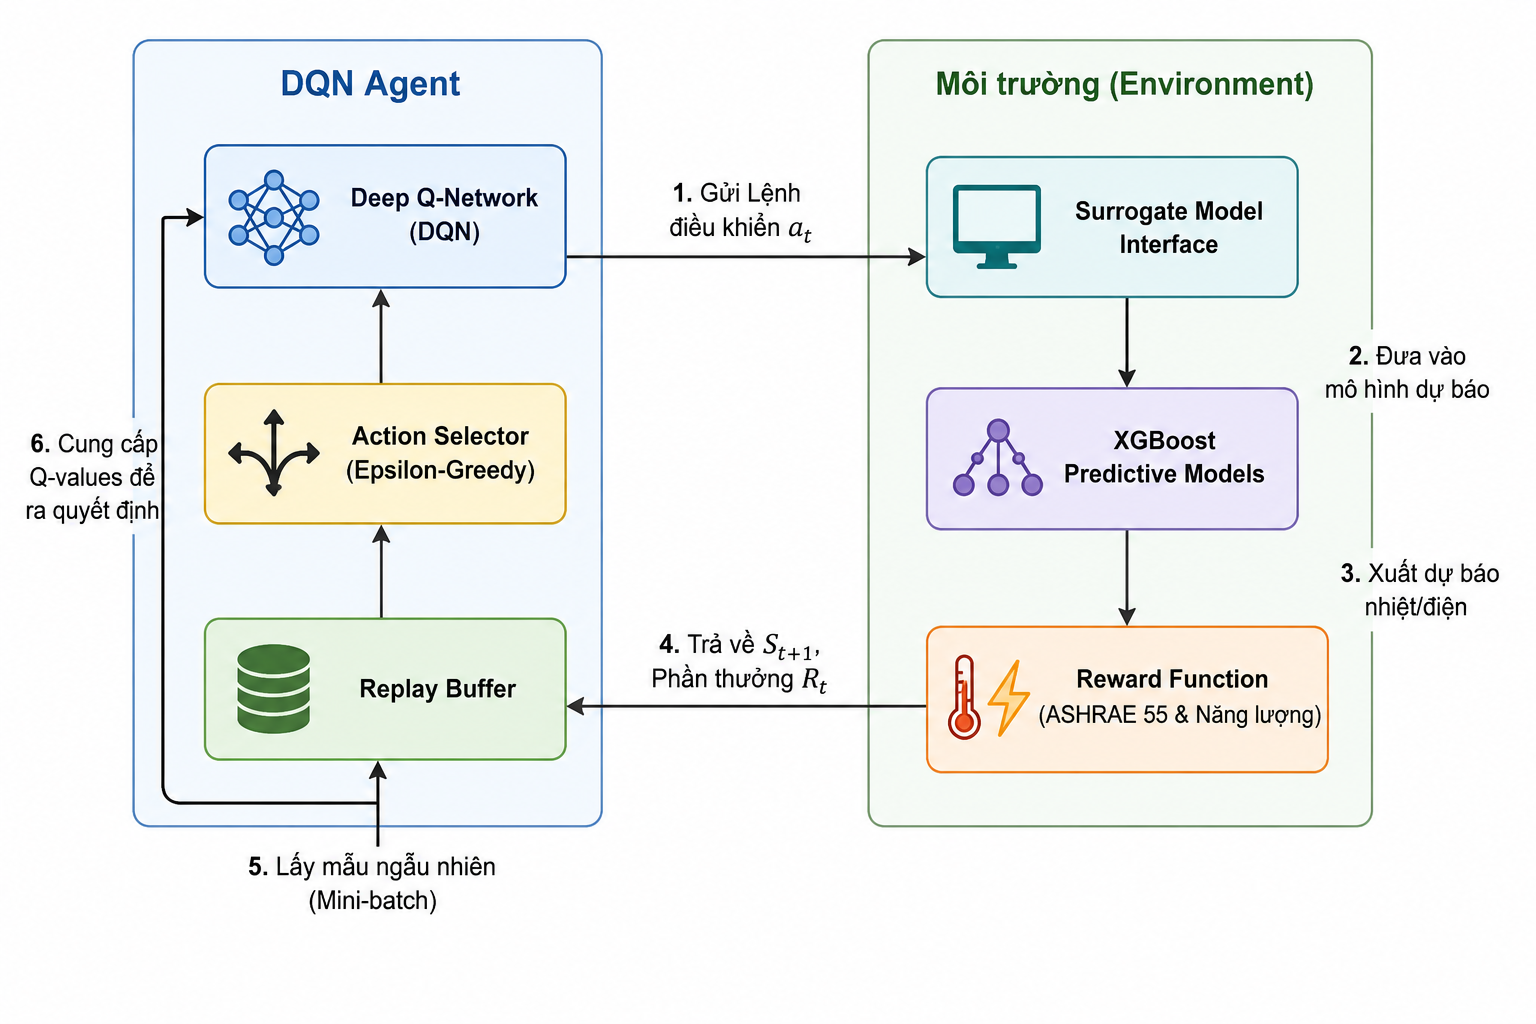
\includegraphics[width=0.9\textwidth]{Images/01_overview_architecture.png}
    \caption{Tổng quan kiến trúc hệ thống}
    \label{fig:01_overview}
\end{figure}

\subsection{Luồng Huấn luyện Tổng quan}
Hình \ref{fig:02_main_loop} trình bày luồng thực thi chính trong quá trình huấn luyện AI. Hệ thống liên tục lặp qua các chu kỳ (Episode), mỗi chu kỳ mô phỏng quá trình tương tác trong nhiều bước thời gian. Tại mỗi bước, tác tử quyết định hành động, môi trường phản hồi và dữ liệu được lưu vào Replay Buffer để lấy mẫu huấn luyện mạng DQN. Hệ số khám phá Epsilon sẽ được giảm dần theo thời gian để tác tử chuyển từ trạng thái học hỏi sang khai thác mô hình \cite{dqn}.

\begin{figure}[H]
    \centering
    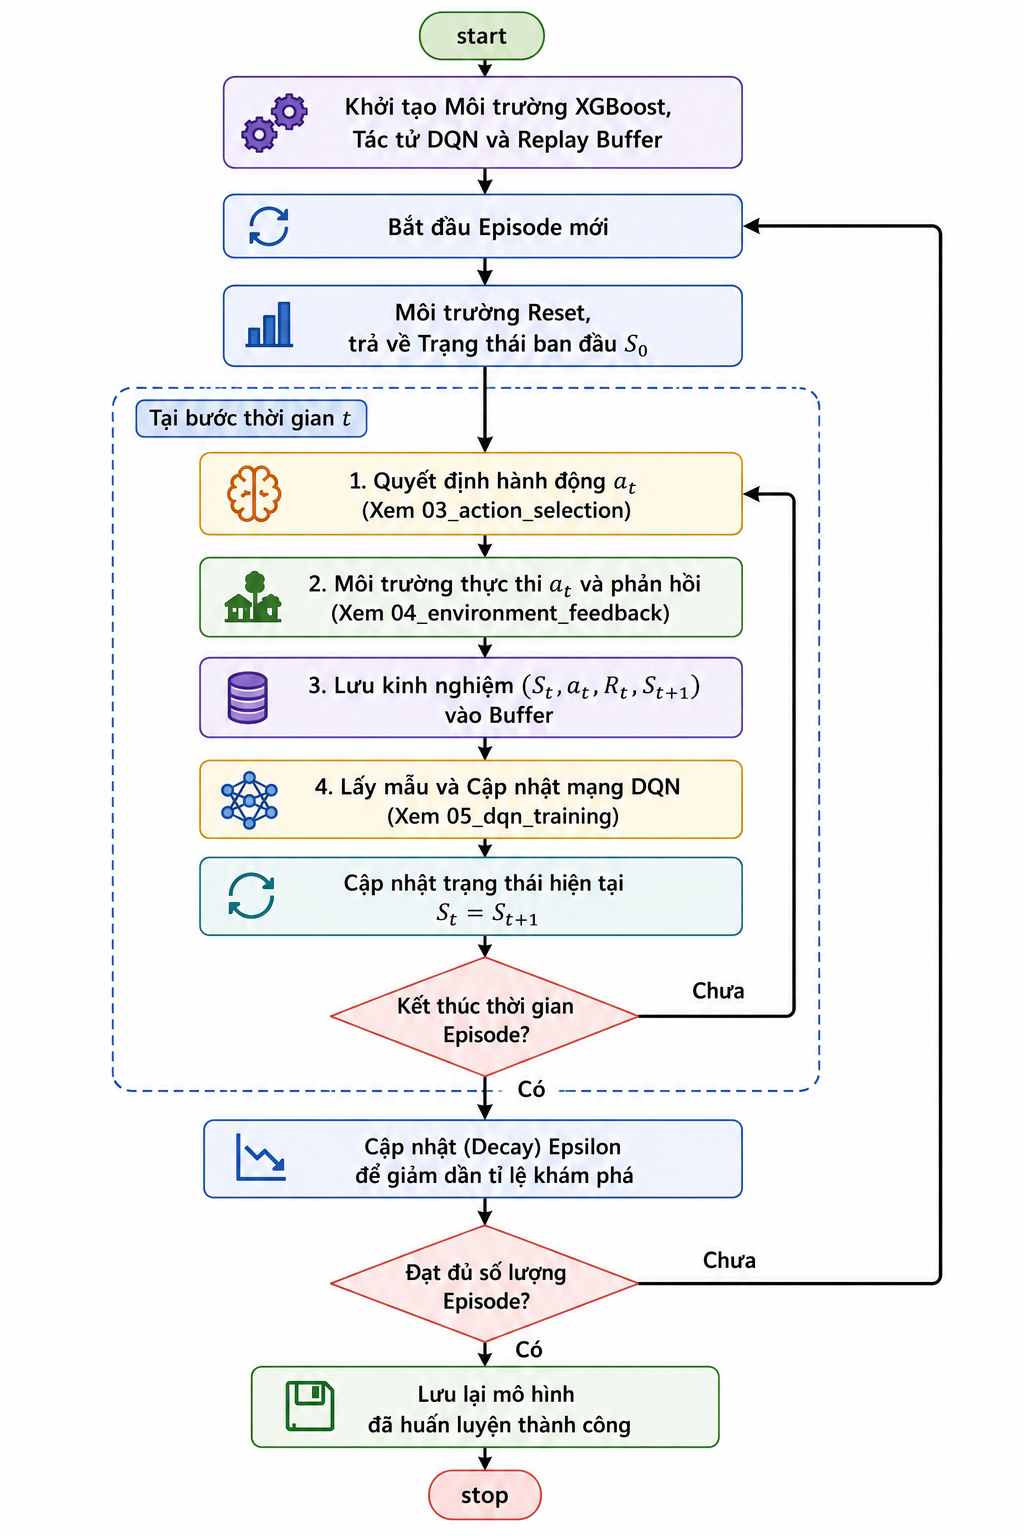
\includegraphics[width=0.7\textwidth]{Images/02_main_training_loop.png}
    \caption{Sơ đồ luồng huấn luyện tổng quan}
    \label{fig:02_main_loop}
\end{figure}

\subsection{Chi tiết Quá trình Ra quyết định}
Hình \ref{fig:03_action_selection} mô tả thuật toán chọn lựa hành động sử dụng chiến lược Epsilon-Greedy. Hệ thống sinh một số ngẫu nhiên để quyết định xem tác tử sẽ chọn hành động ngẫu nhiên (để khám phá các không gian hành vi mới) hay sử dụng mạng DQN dự báo ra hành động tối ưu nhất (có giá trị Q lớn nhất). Hành động sau đó được giải mã để cho ra thiết lập bật/tắt AC, nhiệt độ Setpoint ($20^\circ\text{C}-30^\circ\text{C}$), và trạng thái cửa sổ \cite{dqn}.

\begin{figure}[H]
    \centering
    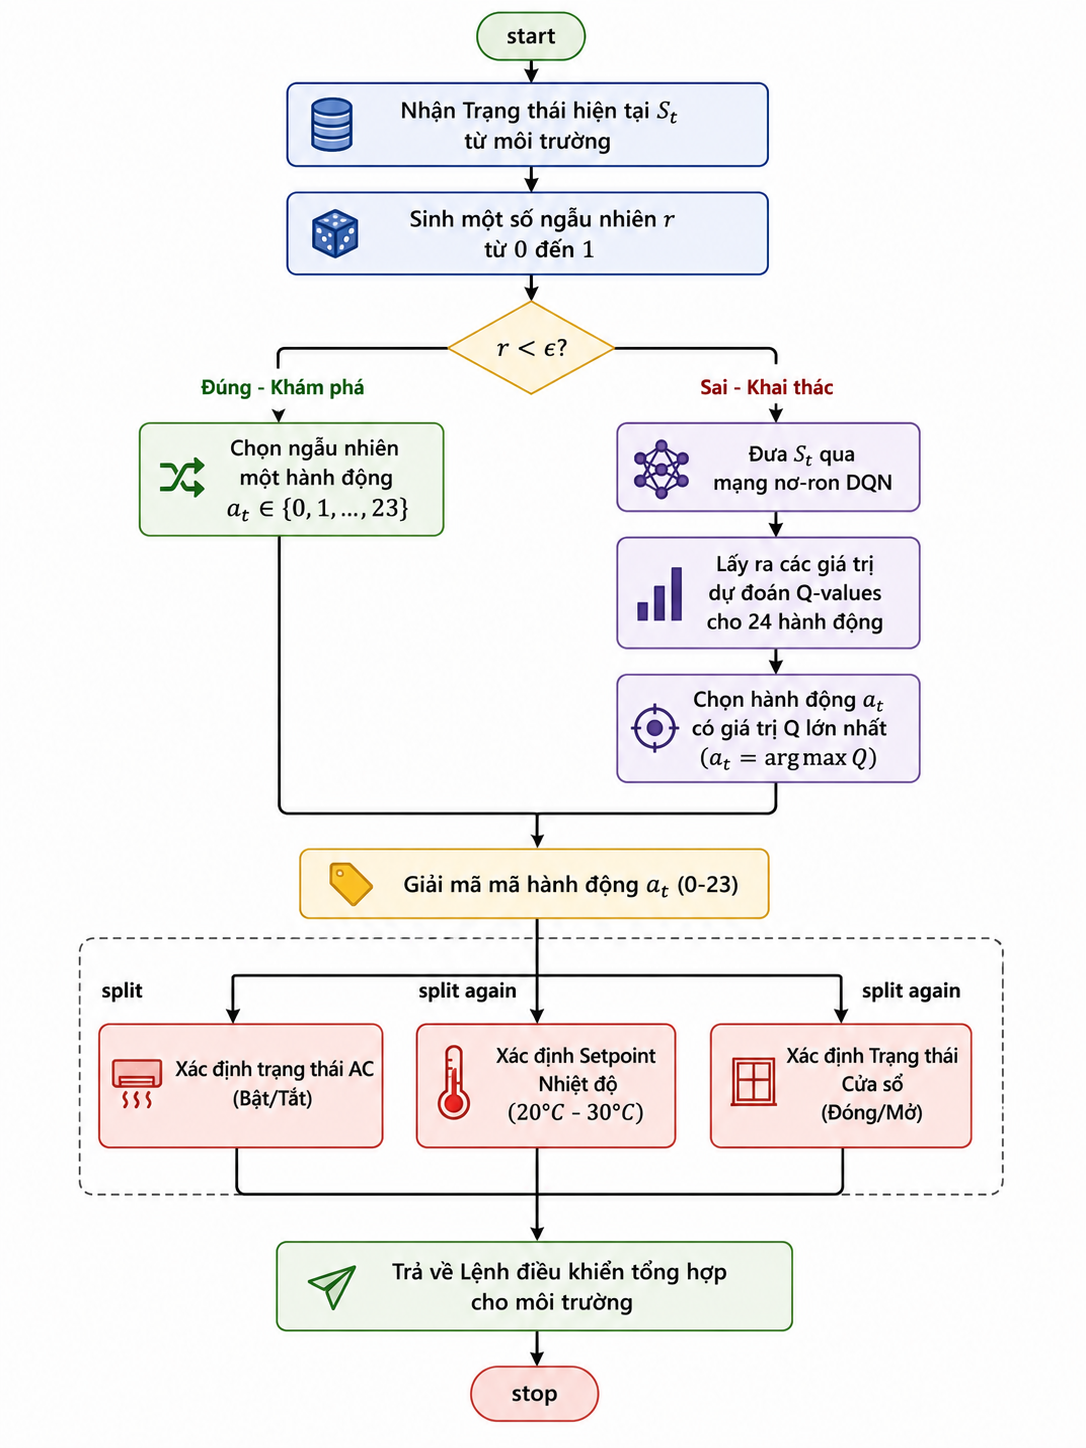
\includegraphics[width=0.7\textwidth]{Images/03_action_selection_detail.png}
    \caption{Chi tiết quá trình ra quyết định của tác tử}
    \label{fig:03_action_selection}
\end{figure}

\subsection{Môi trường Thực thi và Phản hồi}
Hình \ref{fig:04_env_feedback} thể hiện luồng xử lý bên trong môi trường Surrogate. Sau khi nhận lệnh điều khiển, mô hình XGBoost sẽ dự báo trạng thái tiếp theo của tòa nhà. Hệ thống đọc các giá trị nhiệt độ, độ ẩm phòng kết hợp với thời tiết ngoài trời để kiểm tra dải chuẩn ASHRAE 55. Từ đó tính toán Mức phạt Tiện nghi (Penalty Comfort) và Mức phạt Năng lượng (Penalty Energy) và tổng hợp thành phần thưởng $R_t$ \cite{xgboost,ashrae55,whulx}.

\begin{figure}[H]
    \centering
    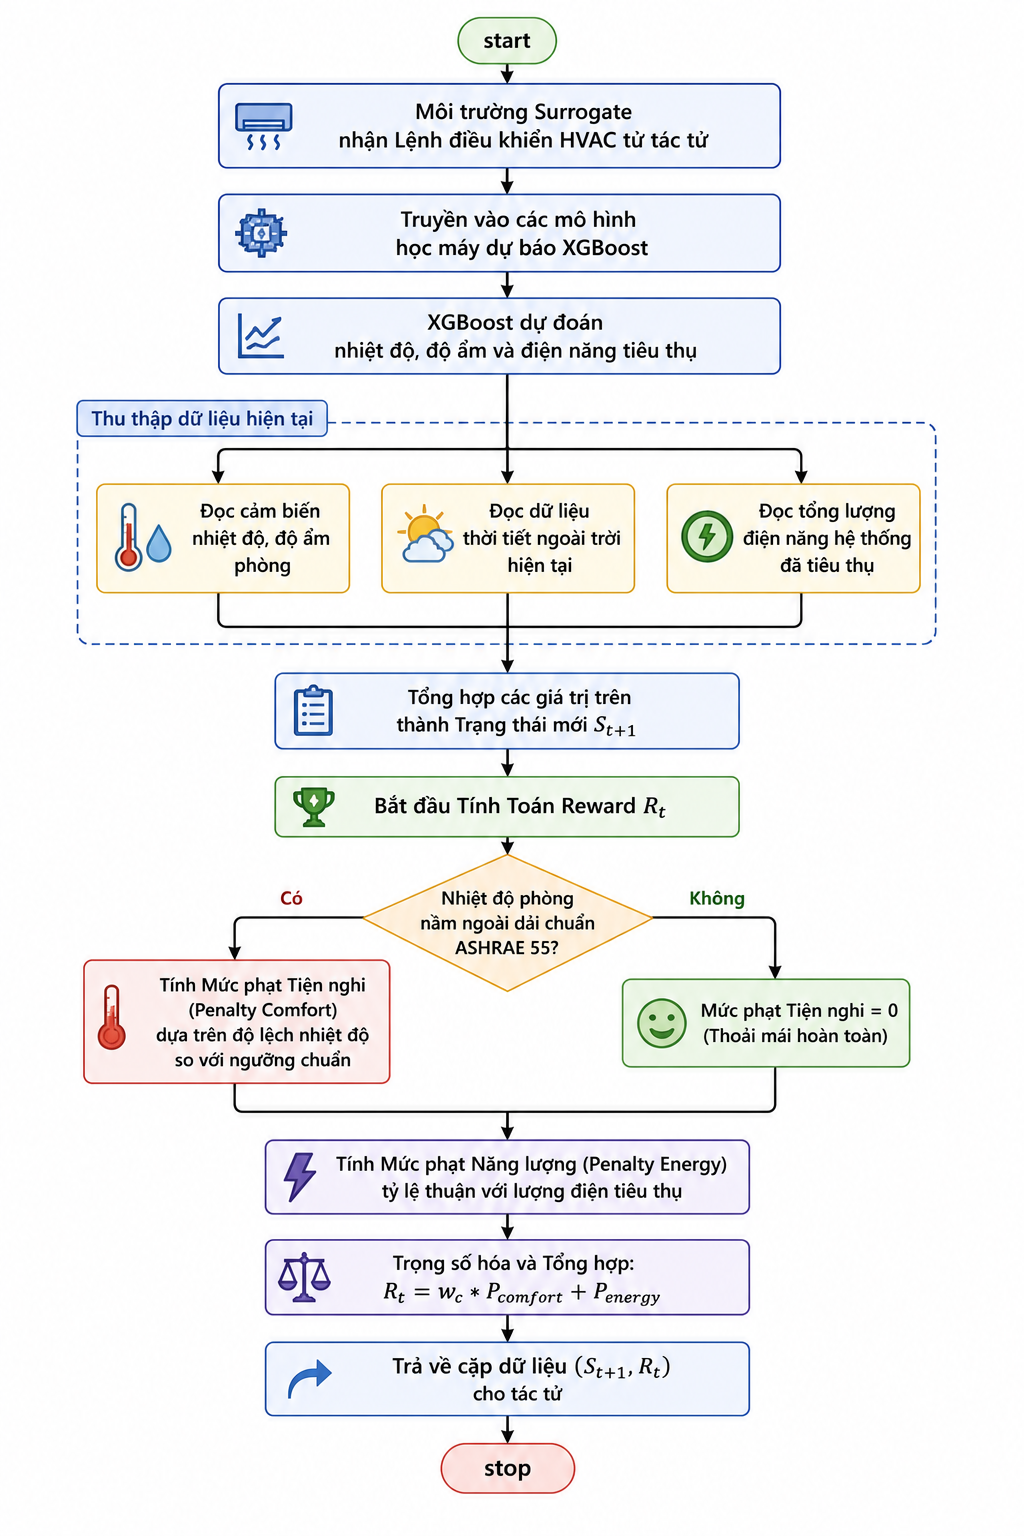
\includegraphics[width=0.7\textwidth]{Images/04_environment_feedback_detail.png}
    \caption{Chi tiết luồng phản hồi từ môi trường Surrogate XGBoost}
    \label{fig:04_env_feedback}
\end{figure}

\subsection{Quá trình Cập nhật Mạng DQN}
Quá trình cập nhật trọng số của lõi mạng trí tuệ nhân tạo được chi tiết ở Hình \ref{fig:05_dqn_training}. Khối Replay Buffer cung cấp các batch dữ liệu ngẫu nhiên (ví dụ 32 mẫu). Mạng Main DQN tính toán Q-value hiện tại, trong khi mạng Target DQN ước tính Q-value kỳ vọng tương lai. Sai số (Loss MSE) giữa hai giá trị này được đạo hàm và tối ưu bằng bộ giảm chấn Adam. Mạng Target DQN cũng được đồng bộ trọng số định kỳ từ mạng Main DQN để ổn định quá trình học \cite{dqn,adam}.

\begin{figure}[H]
    \centering
    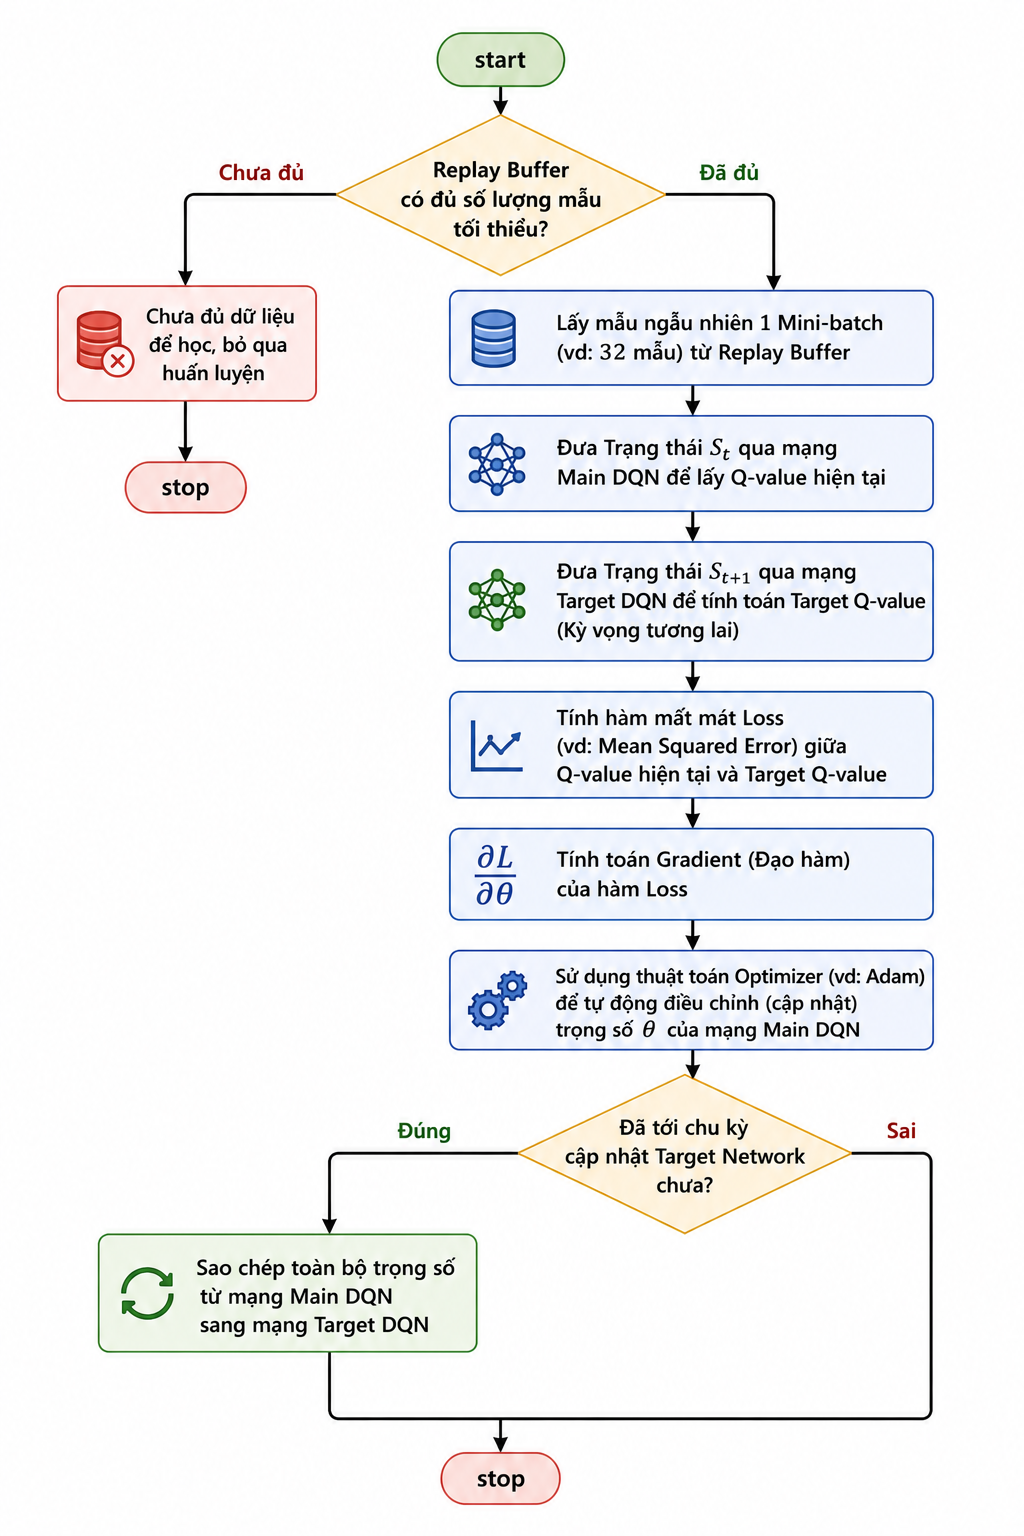
\includegraphics[width=0.7\textwidth]{Images/05_dqn_training_detail.png}
    \caption{Chi tiết quá trình cập nhật mạng DQN}
    \label{fig:05_dqn_training}
\end{figure}

\chapter{Kết quả thực nghiệm và thảo luận}

\textit{Chương này trình bày kết quả thực nghiệm tái hiện mô hình lai XGB-DQN của bài báo gốc \cite{whulx} trên 4 thành phố khảo sát: Rende, Florianopolis, Sao Paulo và Nanjing. Để kiểm chứng hiệu năng, nhóm nghiên cứu đã đối chiếu kết quả của tác tử DQN cải tiến (sau khi áp dụng 4 kỹ thuật sửa lỗi cốt lõi đã đề xuất ở Chương 4) với mô hình DQN gốc gặp lỗi của bài báo và chiến lược vận hành thực tế của con người.}

\section{Đánh giá hiệu năng thuật toán XGB-DQN}

\subsection{Độ chính xác dự báo của mô hình XGBoost (Surrogate Model)}
Hiệu năng điều khiển của tác tử XGB-DQN phụ thuộc mật thiết vào độ chính xác dự báo của mô hình surrogate XGBoost. Tương tự như bài báo gốc, nhóm nghiên cứu đã xây dựng và đánh giá bốn phương án mô hình hóa khác nhau dựa trên tập đặc trưng và biến mục tiêu \cite{whulx}:
\begin{itemize}
    \item \textbf{Model 1}: Dự báo trực tiếp nhiệt độ phòng bước tiếp theo ($T_{in,t+1}$), sử dụng tập đặc trưng thô (Raw features).
    \item \textbf{Model 2}: Dự báo trực tiếp nhiệt độ phòng bước tiếp theo ($T_{in,t+1}$), sử dụng tập đặc trưng cải tiến (Feature-engineered).
    \item \textbf{Model 3}: Dự báo độ biến thiên nhiệt độ ($\Delta T_{in}$), sử dụng tập đặc trưng thô (Raw features).
    \item \textbf{Model 4}: Dự báo độ biến thiên nhiệt độ ($\Delta T_{in}$), sử dụng tập đặc trưng cải tiến (Feature-engineered). \textbf{(Mô hình tối ưu được chọn)}
\end{itemize}

Kết quả huấn luyện và đánh giá 4 mô hình XGBoost trên dữ liệu gốc được thể hiện ở Bảng~\ref{tab:xgb_4models} và biểu đồ khớp chuỗi thời gian gốc ở Hình~\ref{fig:paper_fig4}.

\begin{table}[H]
    \centering
    \caption{Kết quả đánh giá sai số của 4 phương án mô hình XGBoost trên dữ liệu gốc (Bài báo \cite{whulx})}
    \label{tab:xgb_4models}
    \vspace{0.2cm}
    \resizebox{\textwidth}{!}{%
    \begin{tabular}{|l|cc|cc|cc|cc|}
        \hline
        \multirow{2}{*}{\textbf{Chỉ số}} 
            & \multicolumn{2}{c|}{\textbf{Model 1}} 
            & \multicolumn{2}{c|}{\textbf{Model 2}} 
            & \multicolumn{2}{c|}{\textbf{Model 3}} 
            & \multicolumn{2}{c|}{\textbf{Model 4}} \\
        \cline{2-9}
            & \small Train & \small Test 
            & \small Train & \small Test 
            & \small Train & \small Test 
            & \small Train & \small Test \\
        \hline
        MAE ($^\circ$C) & 0.1733 & 0.2444 & 0.1244 & 0.1910 & 0.1682 & 0.2381 & 0.1174 & \textbf{0.1832} \\
        RMSE ($^\circ$C) & 0.2946 & 0.4617 & 0.2047 & 0.3640 & 0.2898 & 0.4678 & 0.1970 & \textbf{0.3561} \\
        $R^2$ & 0.9908 & 0.9769 & 0.9955 & 0.9856 & 0.6961 & 0.1188 & 0.8595 & \textbf{0.4894} \\
        \hline
    \end{tabular}%
    }
\end{table}

\begin{figure}[H]
    \centering
    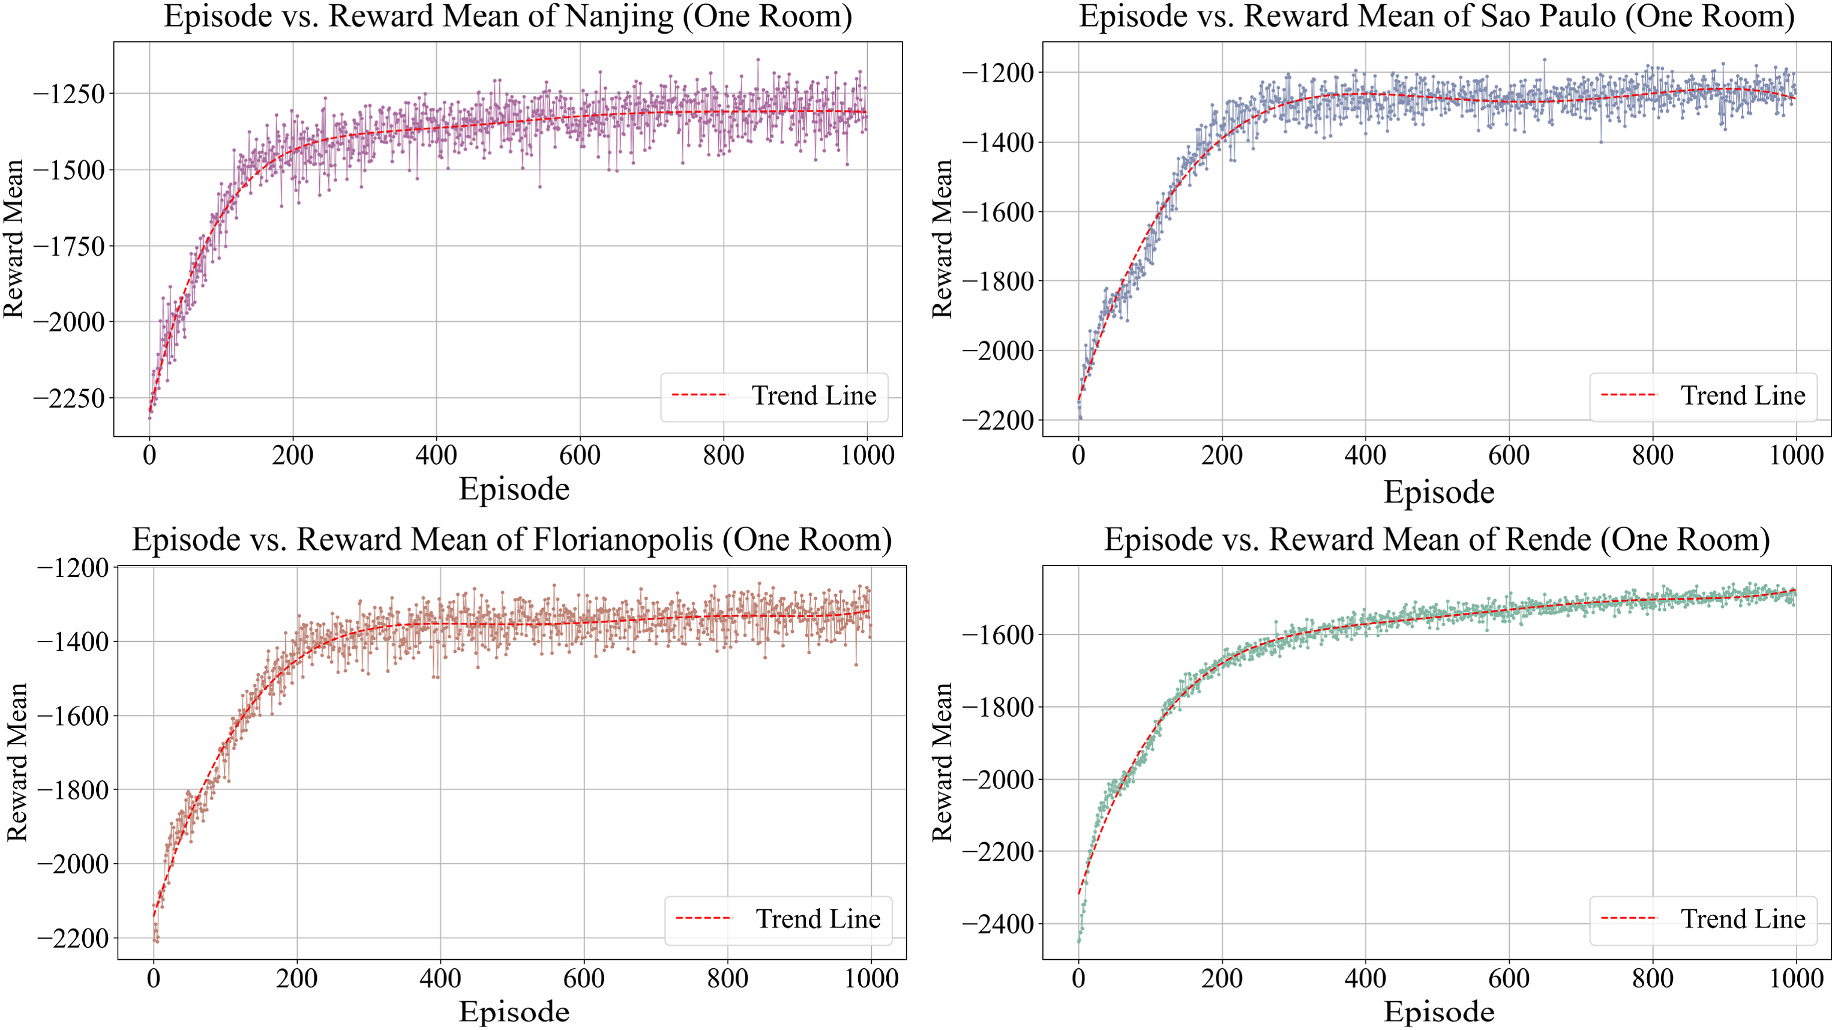
\includegraphics[width=0.95\textwidth]{Images/paper_fig4.jpg}
    \caption{Hiệu năng khớp chuỗi thời gian (60 bước liên tục) của 4 phương án mô hình XGBoost trong bài báo gốc \cite{whulx}.}
    \label{fig:paper_fig4}
\end{figure}

\noindent
\textbf{Thảo luận về hiện tượng tự tương quan thời gian (Temporal Autocorrelation):}
Như đã phân tích ở Chương 3, mặc dù Model 1 và Model 2 đạt hệ số xác định $R^2$ cực cao trên tập kiểm thử (lần lượt là $0.9769$ và $0.9856$), đây thực chất là một ``bẫy thống kê'' do biến nhiệt độ phòng có tính tự tương quan rất mạnh với giá trị ở bước thời gian liền trước ($T_{in,t}$). Khi sử dụng Model 1 hoặc 2 làm surrogate model để mô phỏng tương tác liên tục nhiều bước trong RL (rollout), sai số dự báo sẽ tích lũy theo cấp số nhân khiến nhiệt độ phòng nhanh chóng bị trôi tự do và lệch hoàn toàn so với thực tế (như thể hiện ở đường nét đứt của Model 1 và 2 trong Hình~\ref{fig:paper_fig4}).

Ngược lại, Model 3 và Model 4 triệt tiêu hoàn toàn ảnh hưởng của tự tương quan bằng cách dự báo độ biến thiên $\Delta T_{in}$. Mặc dù $R^2$ của hai mô hình này trông thấp hơn nhiều ($0.1188$ và $0.4894$), chúng phản ánh chính xác khả năng học và khớp xu hướng vật lý thực tế. Nhờ áp dụng feature engineering (bổ sung các đặc trưng phái sinh như thời gian AC chạy liên tục \texttt{CLast\_Time\_T}, thời gian cửa sổ mở liên tục, biến tháng, biến giờ trong ngày), \textbf{Model 4} đã giảm RMSE từ $0.4678^\circ$C xuống $0.3561^\circ$C và tăng $R^2$ đáng kể lên $0.4894$. Kết quả đánh giá trên dữ liệu của bài báo gốc cũng ghi nhận xu hướng tương đồng với MAE kiểm thử của Model 4 đạt $0.1832^\circ$C, xác nhận độ tin cậy của mô hình surrogate được lựa chọn.

\subsection{Sự hội tụ của XGB-DQN qua đường cong phần thưởng}
Đường cong phần thưởng tích lũy trung bình qua các episode huấn luyện là chỉ số quan trọng phản ánh tiến trình học tập và độ ổn định của tác tử RL. Hình~\ref{fig:paper_fig5} trình bày các đường cong phần thưởng huấn luyện tại 4 thành phố trong bài báo gốc.

\begin{figure}[H]
    \centering
    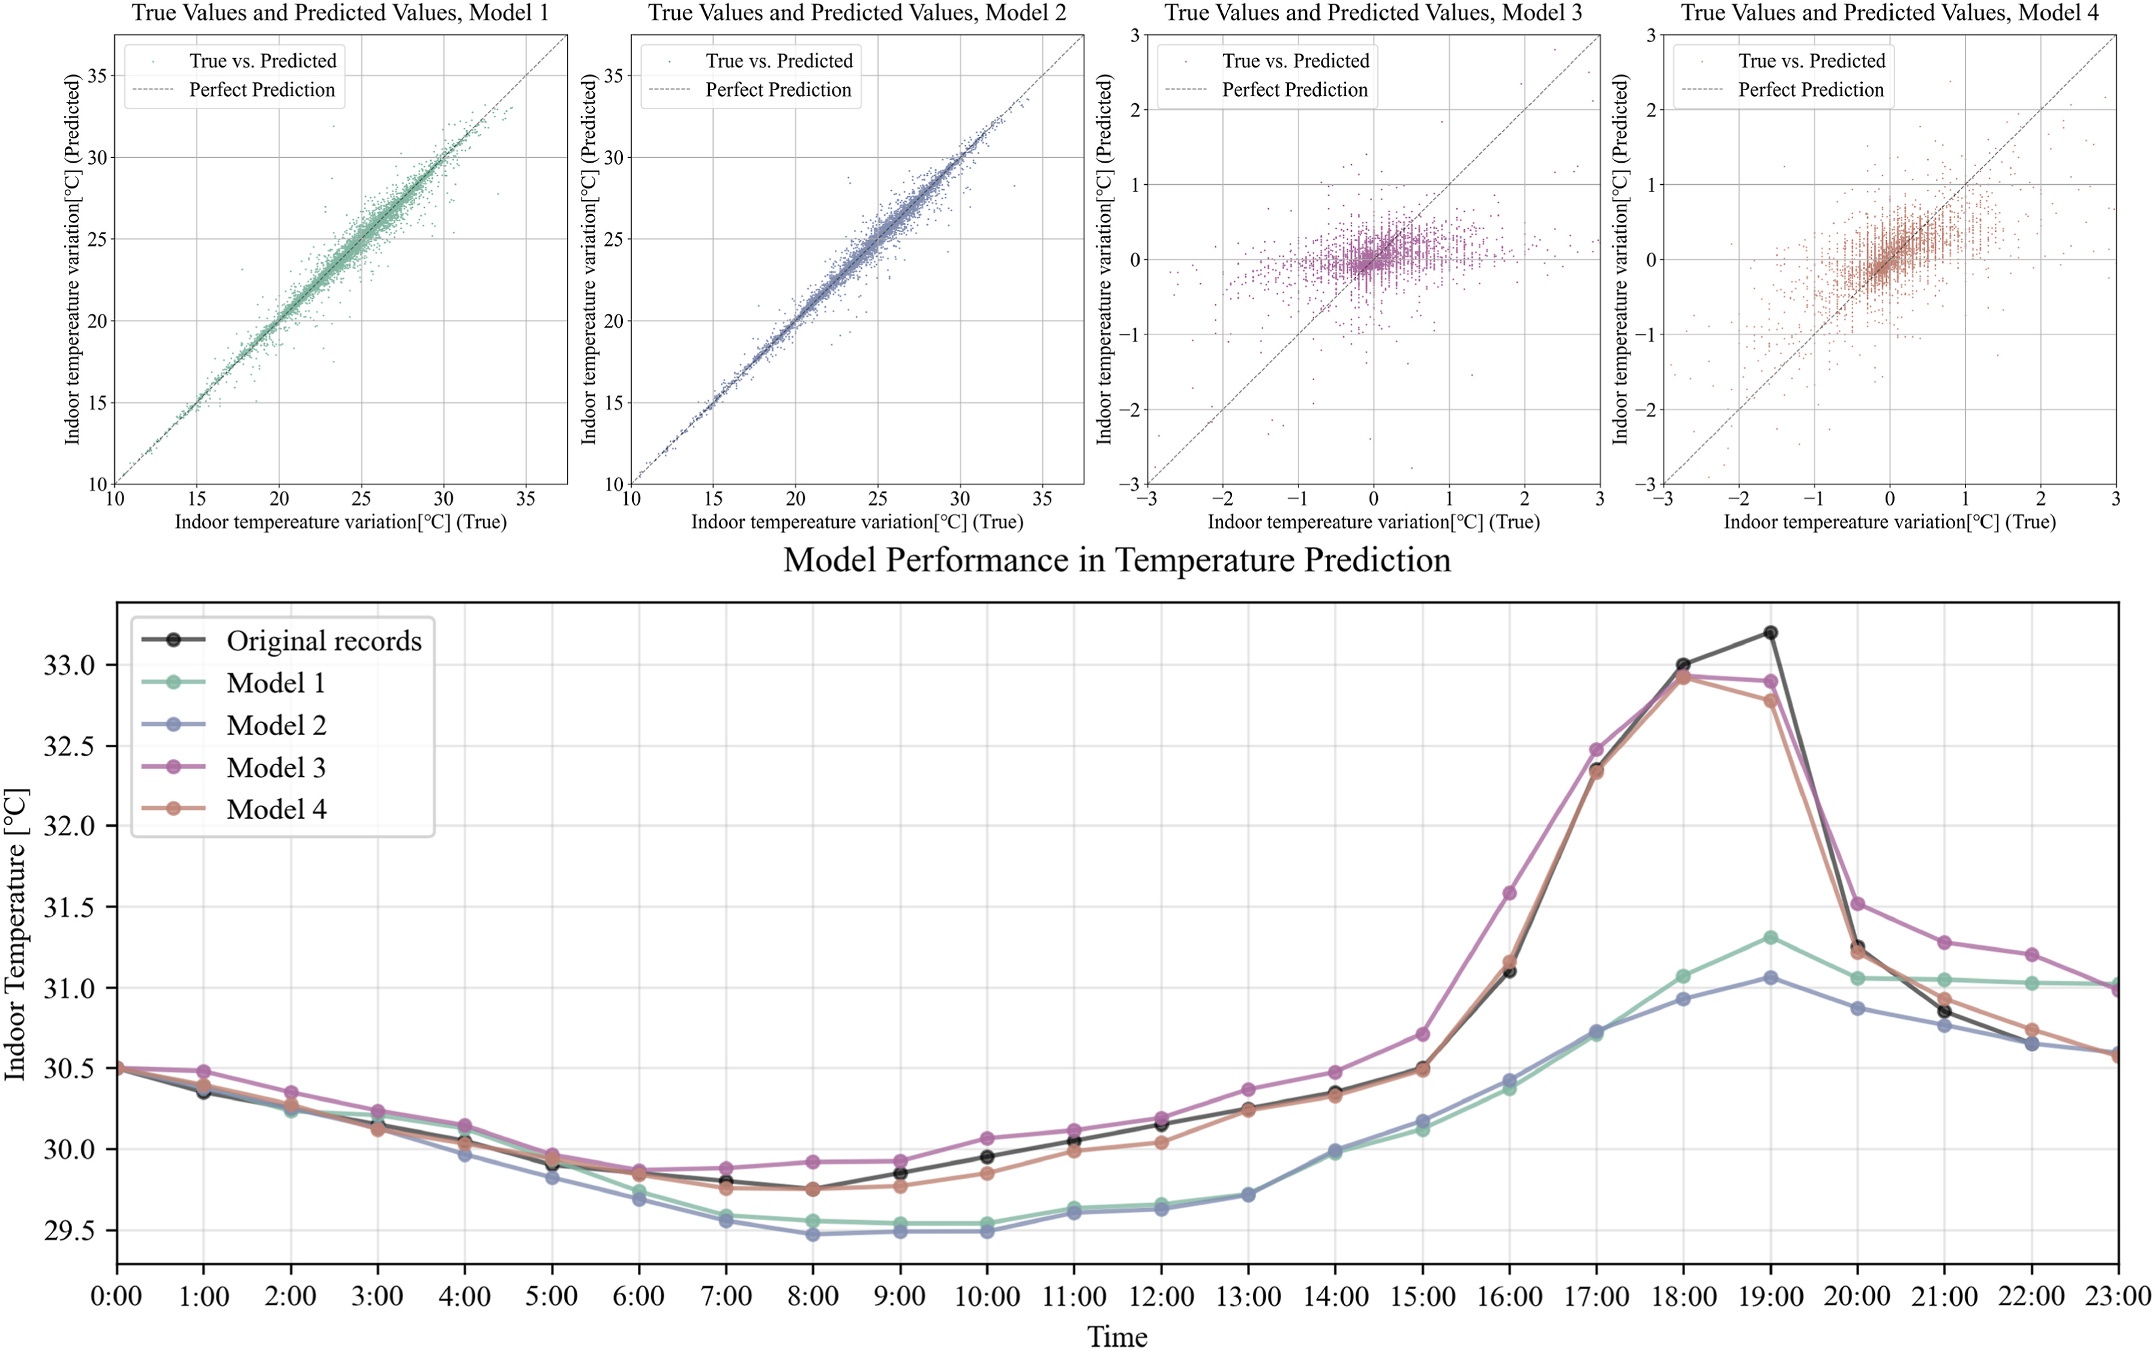
\includegraphics[width=0.92\textwidth]{Images/paper_fig5.jpg}
    \caption{Đường cong phần thưởng tích lũy của tác tử XGB-DQN tại 4 đô thị khảo sát trong bài báo gốc \cite{whulx}.}
    \label{fig:paper_fig5}
\end{figure}

\noindent
\textbf{Phân tích tiến trình hội tụ:}
Trong giai đoạn đầu huấn luyện (từ episode 1 đến 200), do hệ số khám phá ngẫu nhiên $\epsilon$ còn lớn ($\epsilon > 0.8$), tác tử thực hiện khám phá không gian hành động một cách ngẫu nhiên. Điều này dẫn đến điểm thưởng trung bình nhận được rất thấp và dao động cực kỳ mạnh. 
Khi số lượng episode tăng lên và $\epsilon$ giảm dần (giai đoạn từ episode 300 đến 700), tác tử bắt đầu khai thác các kinh nghiệm thành công lưu trữ trong Replay Buffer, điểm thưởng tăng dần một cách rõ rệt.
Ở giai đoạn cuối (episode 700 trở đi, khi $\epsilon$ tiệm cận mức tối thiểu $0.01$), các đường cong phần thưởng của bài báo gốc (Hình~\ref{fig:paper_fig5}) đều đi vào vùng ổn định phẳng. Sự hội tụ này chứng tỏ tác tử DQN cải tiến sau khi áp dụng các đề xuất sửa lỗi thuật toán đã học được chính sách (policy) điều khiển tối ưu và ổn định toán học, vượt qua hiện tượng bùng nổ gradient nhờ sự hỗ trợ của mạng Target Q-Network.

\section{Tối ưu hóa hiệu năng và khả năng tiết kiệm năng lượng}

\subsection{Duy trì và cải thiện tiện nghi nhiệt trong nhà}
Mục tiêu hàng đầu của hệ thống điều khiển HVAC thông minh là đảm bảo tiện nghi nhiệt thích ứng cho người dùng trong thời gian làm việc. Hình~\ref{fig:paper_fig6} thể hiện biểu đồ phân bố nhiệt độ phòng và xác suất kích hoạt điều hòa (AC Activation Probability) của bài báo gốc.

\begin{figure}[H]
    \centering
    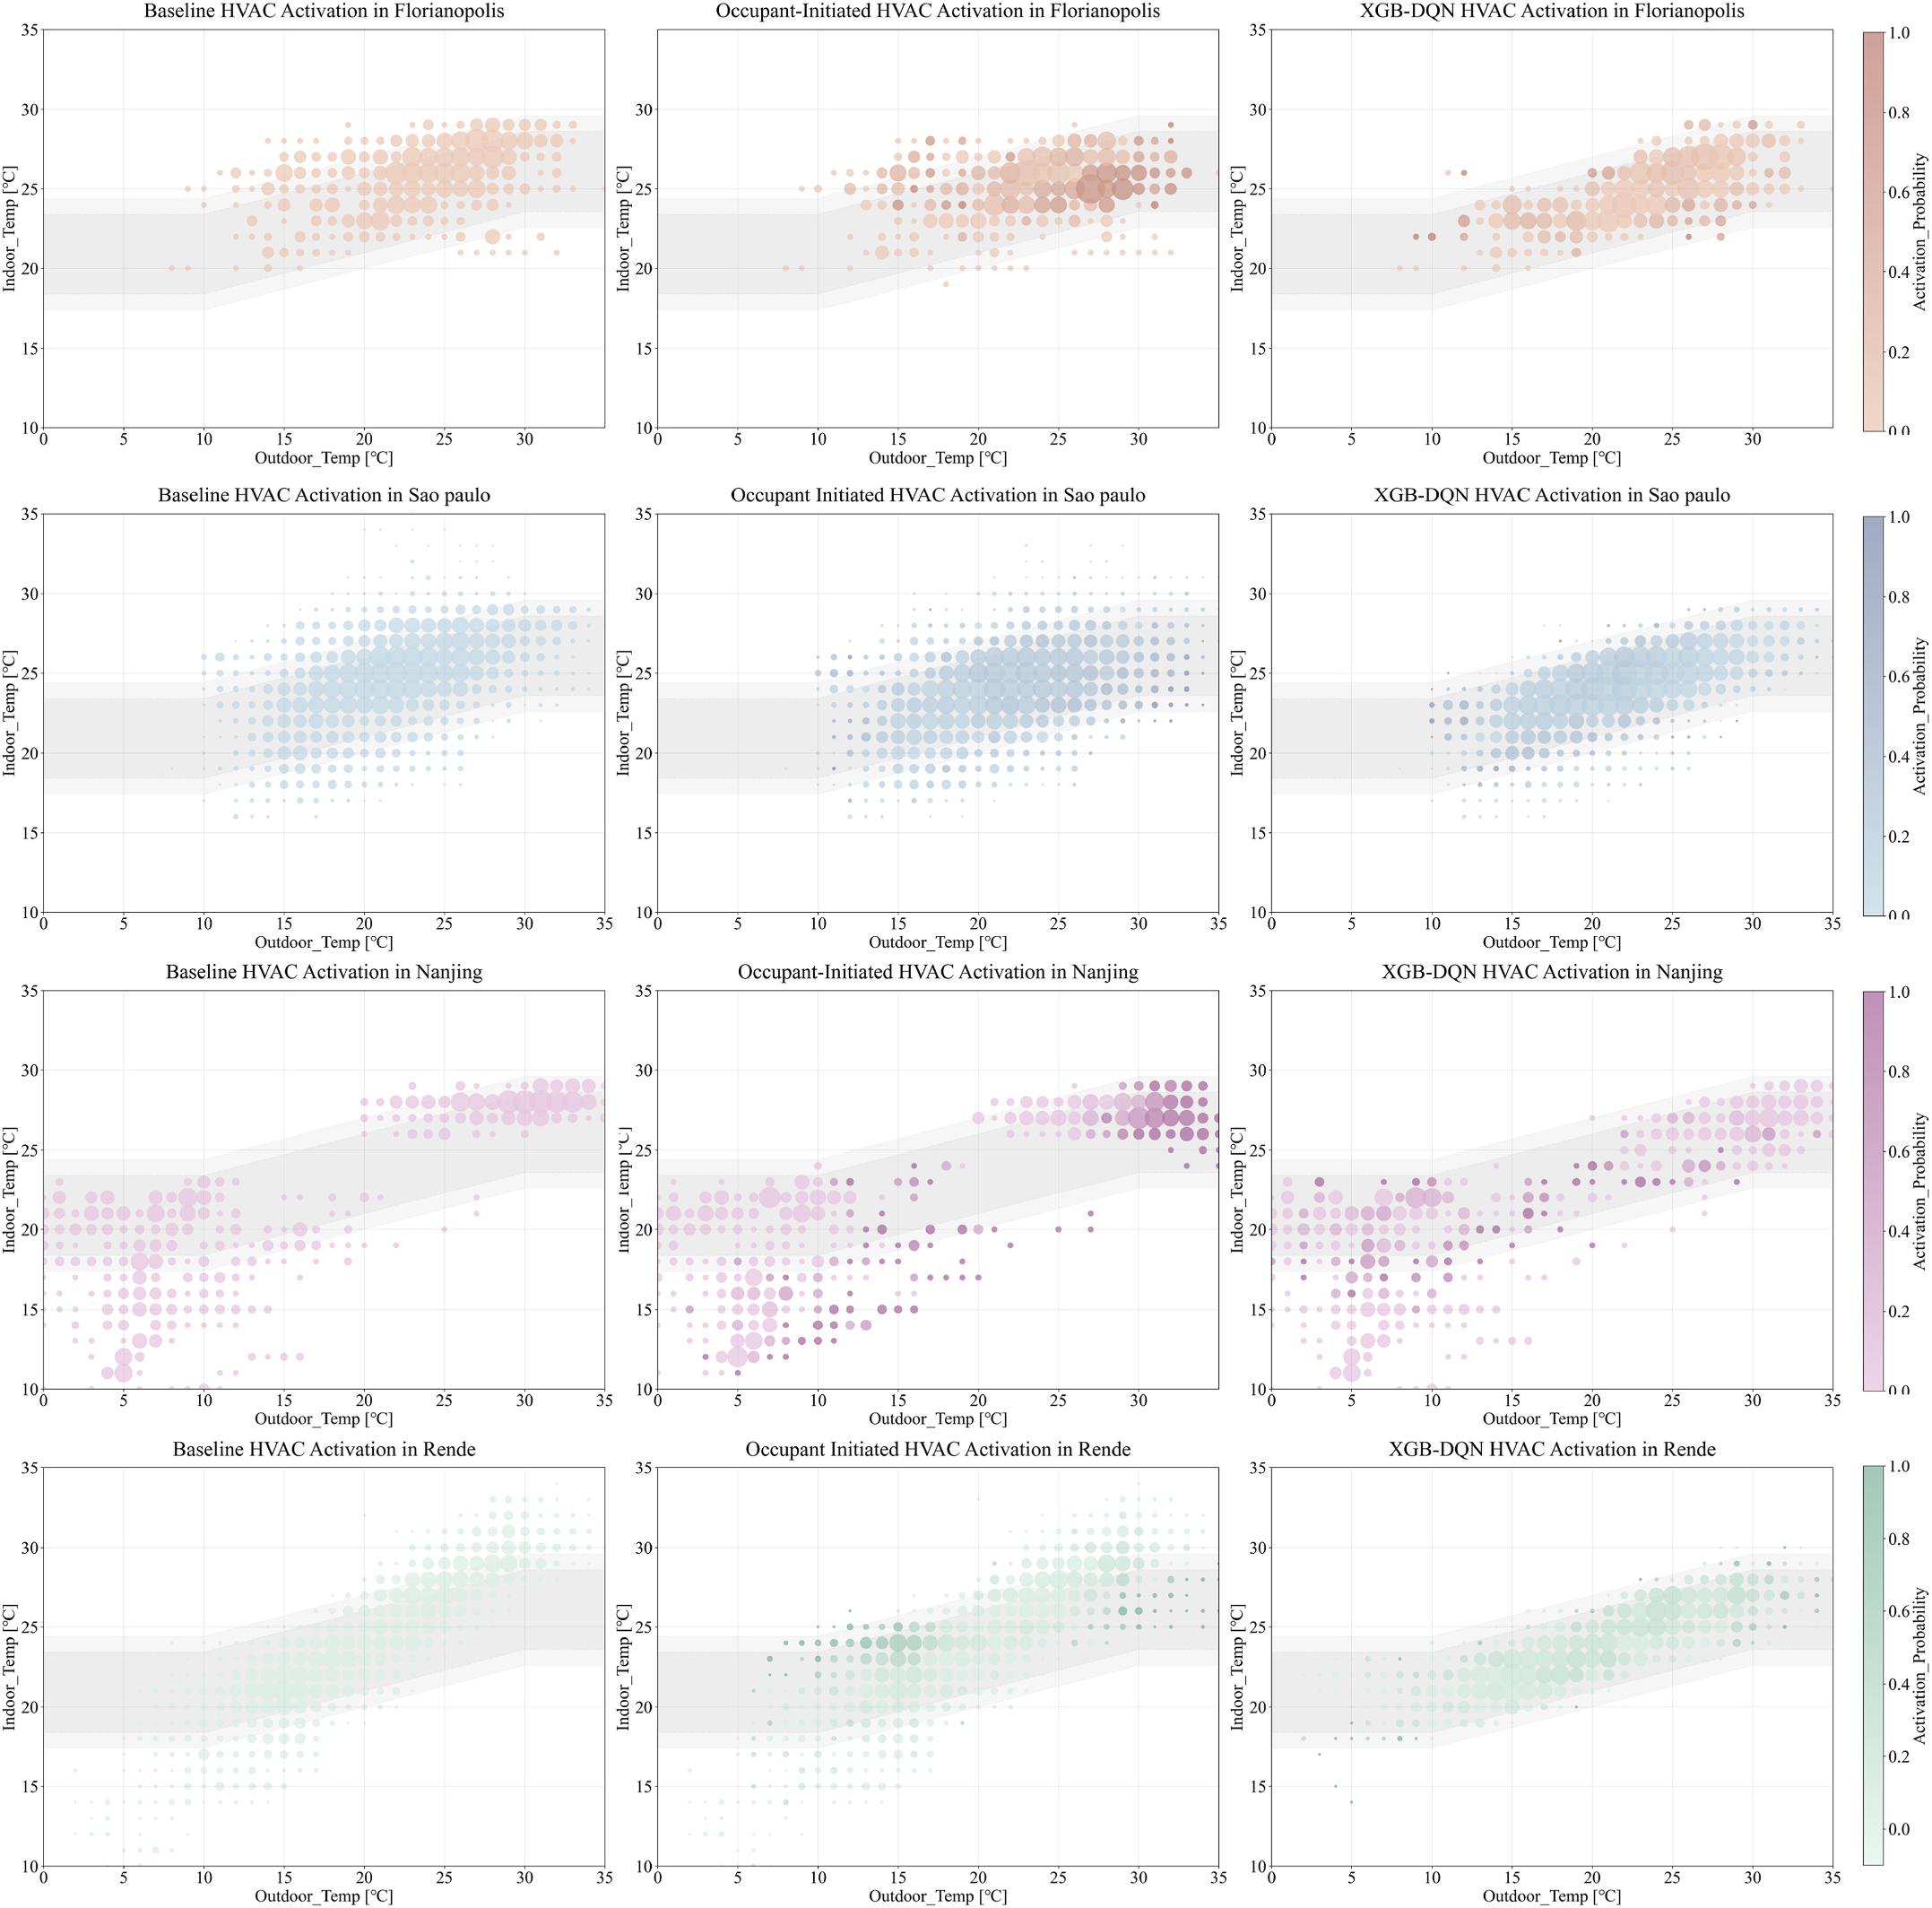
\includegraphics[width=0.95\textwidth]{Images/paper_fig6.jpg}
    \caption{Biểu đồ phân bố nhiệt độ trong nhà--ngoài trời và xác suất bật AC tại 4 thành phố dưới ba kịch bản vận hành (Baseline không can thiệp, Người dùng tự điều khiển và XGB-DQN điều khiển) trong bài báo gốc \cite{whulx}.}
    \label{fig:paper_fig6}
\end{figure}

\noindent
\textbf{Nhận xét từ biểu đồ phân bố nhiệt độ gốc (Hình~\ref{fig:paper_fig6}):}
\begin{itemize}
    \item \textbf{Kịch bản Baseline (Cột 1):} Khi không có sự can thiệp của điều hòa hay cửa sổ, nhiệt độ trong phòng phụ thuộc tuyến tính và trôi tự do theo nhiệt độ môi trường ngoài trời. Một lượng lớn các điểm trạng thái nằm hoàn toàn ngoài dải thoải mái màu xanh lá cây của tiêu chuẩn ASHRAE 55, gây ra tình trạng nóng bức hoặc lạnh giá nghiêm trọng.
    \item \textbf{Kịch bản Người dùng tự điều khiển - Occupant Control (Cột 2):} Người dùng có can thiệp bật/tắt AC và đóng/mở cửa sổ nhưng hành vi này mang tính thụ động, trễ và thiếu tối ưu. Biểu đồ cho thấy xác suất bật AC (biểu thị bằng màu đỏ) phân bố rải rác, không đồng đều, dẫn đến nhiều thời điểm phòng vẫn bị nóng hoặc quá lạnh.
    \item \textbf{Kịch bản XGB-DQN (Cột 3):} Tác tử RL đã kéo thành công phần lớn các điểm trạng thái nhiệt độ phòng tập trung vào đúng dải thoải mái thích ứng (nằm giữa hai đường giới hạn nét đứt màu xanh). Xác suất kích hoạt điều hòa hiển thị màu đỏ đậm tập trung chính xác ở các vùng nhiệt độ ngoài trời cao, và chuyển dần sang màu xanh dương (tắt AC) khi nhiệt độ ngoài trời mát mẻ.
\end{itemize}

\noindent
\textbf{Thảo luận về kết quả tái hiện và sửa lỗi chính sách (0\% AC):}
Để xác minh nguyên nhân toán học của lỗi sụp đổ chính sách của thuật toán gốc (AC On = 0.00\%) do nhóm phát hiện ở Chương 3, nhóm nghiên cứu đã tiến hành huấn luyện và đánh giá đối chứng các thuật toán trên tập dữ liệu kiểm thử dài hạn 1.763 ngày. Kết quả đối chứng được thể hiện chi tiết ở Bảng~\ref{tab:comparison_focused}.

\begin{table}[H]
    \centering
    \caption{Bảng so sánh hiệu năng các bộ điều khiển trên toàn bộ 1.763 ngày đánh giá tái hiện}
    \label{tab:comparison_focused}
    \vspace{0.2cm}
    \resizebox{\textwidth}{!}{%
    \begin{tabular}{|l|c|c|c|c|}
        \hline
        \textbf{Bộ điều khiển} & \textbf{Comfort (\%)} & \textbf{Tỉ lệ bật AC (\%)} & \textbf{Tỉ lệ mở cửa (\%)} & \textbf{Reward trung bình} \\
        \hline
        \textbf{DQN Cải tiến (Nhóm)} & \textbf{78.55\%} & \textbf{66.97\%} & \textbf{30.93\%} & \textbf{-794.45} \\
        \hline
        Human (Thực tế) & 72.84\% & 14.37\% & 52.17\% & \textit{N/A} \\
        \hline
        DQN Gốc (WHU-LX) & 67.99\% & 0.00\% & 34.09\% & -14.51 \\
        \hline
    \end{tabular}%
    }
\end{table}

Số liệu thực nghiệm cho thấy bộ điều khiển DQN Gốc gặp lỗi nghiêm trọng khi đạt tỷ lệ bật điều hòa bằng 0.00\% trên toàn bộ 1.763 ngày thử nghiệm, khiến tỷ lệ tiện nghi nhiệt sụt giảm xuống 67.99\% (thậm chí kém cả kịch bản con người tự vận hành thực tế đạt 72.84\%).
Sau khi áp dụng cải tiến Reward Rescaling ($w_c = 120.0$) kết hợp với chuẩn hóa trạng thái và Target Network, tác tử DQN Cải tiến đã học được chính sách tối ưu: chủ động bật điều hòa trong 66.97\% thời gian nắng nóng để duy trì tiện nghi nhiệt lên mức xuất sắc 78.55\%, vượt trội hơn cả con người và khắc phục triệt để lỗi sụp đổ chính sách.

\subsection{Tiêu thụ năng lượng và chi phí tiền điện ước tính}
Bên cạnh việc duy trì tiện nghi nhiệt, XGB-DQN hướng tới mục tiêu tối ưu hóa hiệu quả sử dụng năng lượng. Bảng~\ref{tab:paper_multi_city_comparison} tổng hợp kết quả đánh giá đa đô thị trong bài báo gốc đối với kịch bản Người dùng tự điều khiển (Scenario-1) và XGB-DQN điều khiển (Scenario-2).

\begin{table}[H]
    \centering
    \caption{Bảng so sánh hiệu năng chi tiết giữa các kịch bản tại 4 đô thị khảo sát (Bài báo gốc \cite{whulx})}
    \label{tab:paper_multi_city_comparison}
    \vspace{0.2cm}
    \resizebox{\textwidth}{!}{%
    \begin{tabular}{|l|c|c|c|c|c|c|}
        \hline
        \textbf{Chỉ số đánh giá} & \textbf{Kịch bản} & \textbf{Rende} & \textbf{Florianopolis} & \textbf{Sao Paulo} & \textbf{Nanjing} & \textbf{Tổng cộng} \\
        \hline
        Tổng số giờ khảo sát (h) & - & 4128.00 & 768.00 & 12732.00 & 900.00 & 18528.00 \\
        \hline
        \multirow{3}{*}{Thời gian bật AC (h)} & Baseline & 0.00 & 0.00 & 0.00 & 0.00 & 0.00 \\
        & Scenario-1 & 592.00 & 227.00 & 2451.00 & 231.00 & 3501.00 \\
        & Scenario-2 & 649.00 & 81.00 & 1762.00 & 144.00 & 2636.00 \\
        \hline
        \multirow{3}{*}{Thời gian mở cửa (h)} & Baseline & 0.00 & 0.00 & 0.00 & 0.00 & 0.00 \\
        & Scenario-1 & 508.00 & 293.00 & 8971.00 & 562.00 & 10334.00 \\
        & Scenario-2 & 1441.00 & 339.00 & 4476.00 & 329.00 & 6585.00 \\
        \hline
        \multirow{3}{*}{Thời lượng tiện nghi (h)} & Baseline & 2571.00 & 561.00 & 9119.00 & 517.00 & 12768.00 \\
        & Scenario-1 & 2599.00 & 613.00 & 9626.00 & 659.00 & 13497.00 \\
        & Scenario-2 & 4040.00 & 735.00 & 11827.00 & 620.00 & 17222.00 \\
        \hline
        \multirow{2}{*}{Tỷ lệ cải thiện tiện nghi $TC$ (\%)} & Scenario-1 & 1\% & 7\% & 4\% & 16\% & 4\% \\
        & Scenario-2 & \textbf{36\%} & \textbf{23\%} & \textbf{21\%} & \textbf{11\%} & \textbf{24\%} \\
        \hline
        \multirow{2}{*}{Điện năng tiêu thụ $EC_{abs}$ (kWh)} & Scenario-1 & 888.00 & 195.22 & 2107.86 & 166.32 & 3357.40 \\
        & Scenario-2 & 973.50 & 69.66 & 1515.32 & 103.68 & 2662.16 \\
        \hline
        \multirow{2}{*}{Năng lượng tương đối $EC_{rel}$ (kW)} & Scenario-1 & 0.34 & 0.32 & 0.22 & 0.25 & 0.28 \\
        & Scenario-2 & \textbf{0.24} & \textbf{0.09} & \textbf{0.13} & \textbf{0.17} & \textbf{0.16} \\
        \hline
        \multirow{2}{*}{Chi phí điện ước tính năm (\$)} & Scenario-1 & 1113.70 & 327.36 & 213.19 & 124.68 & 414.25 \\
        & Scenario-2 & 1220.93 & 116.80 & 153.26 & 77.67 & 385.95 \\
        \hline
    \end{tabular}%
    }
    \\[0.1cm]
    {\small \textit{Ghi chú: Scenario-1 ứng với Người dùng tự vận hành thực tế; Scenario-2 ứng với XGB-DQN điều khiển.}}
\end{table}

\noindent
\textbf{Phân tích hiệu quả năng lượng đa đô thị:}
Theo số liệu từ Bảng~\ref{tab:paper_multi_city_comparison}, ngoại trừ Rende, hệ thống XGB-DQN giúp giảm thời gian hoạt động của AC tổng cộng **780 giờ** (giảm **32\%**) ở 3 đô thị còn lại. Điều này mang lại mức tiết kiệm tiền điện hàng năm cực kỳ ấn tượng: Florianopolis giảm **64.5\%** chi phí (tiết kiệm **\$211**), Sao Paulo giảm **28\%** (tiết kiệm **\$60**) và Nanjing giảm **37.9\%** (tiết kiệm **\$47**).

Trường hợp đặc biệt xảy ra tại Rende (Ý): do khí hậu mùa hè Địa Trung Hải vô cùng khắc nghiệt và oi bức, tác tử quyết định tăng thời gian hoạt động của AC thêm **85 giờ** (tăng **9.6\%**) nhằm kéo tỷ lệ tiện nghi tăng vọt thêm **36\%**. Tuy hóa đơn tiền điện của kịch bản XGB-DQN tại Rende tăng thêm **\$107**, chỉ số **Năng lượng tiêu thụ tương đối** $EC_{rel}$ (đo lượng điện năng tiêu hao để đổi lại 1 giờ tiện nghi tăng thêm) vẫn giảm mạnh từ **0.34 kW** xuống **0.24 kW**. Điều này khẳng định tác tử XGB-DQN đã sử dụng điện năng một cách thông minh và hiệu quả hơn hành vi tự phát của con người. Tính trung bình trên cả 4 đô thị, XGB-DQN đã giảm $EC_{rel}$ từ **0.28 kW** xuống còn **0.16 kW** (tiết kiệm **42.8\%**).

\section{Điều khiển phối hợp thông minh giữa HVAC và cửa sổ}
Khả năng điều khiển phối hợp (Collaborative Control) giữa thiết bị cơ điện HVAC và hệ thông gió tự nhiên (cửa sổ) là chìa khóa để đạt hiệu quả năng lượng tối đa. Hình~\ref{fig:paper_fig7} thể hiện bản đồ nhiệt xác suất mở cửa sổ của bài báo gốc.

\begin{figure}[H]
    \centering
    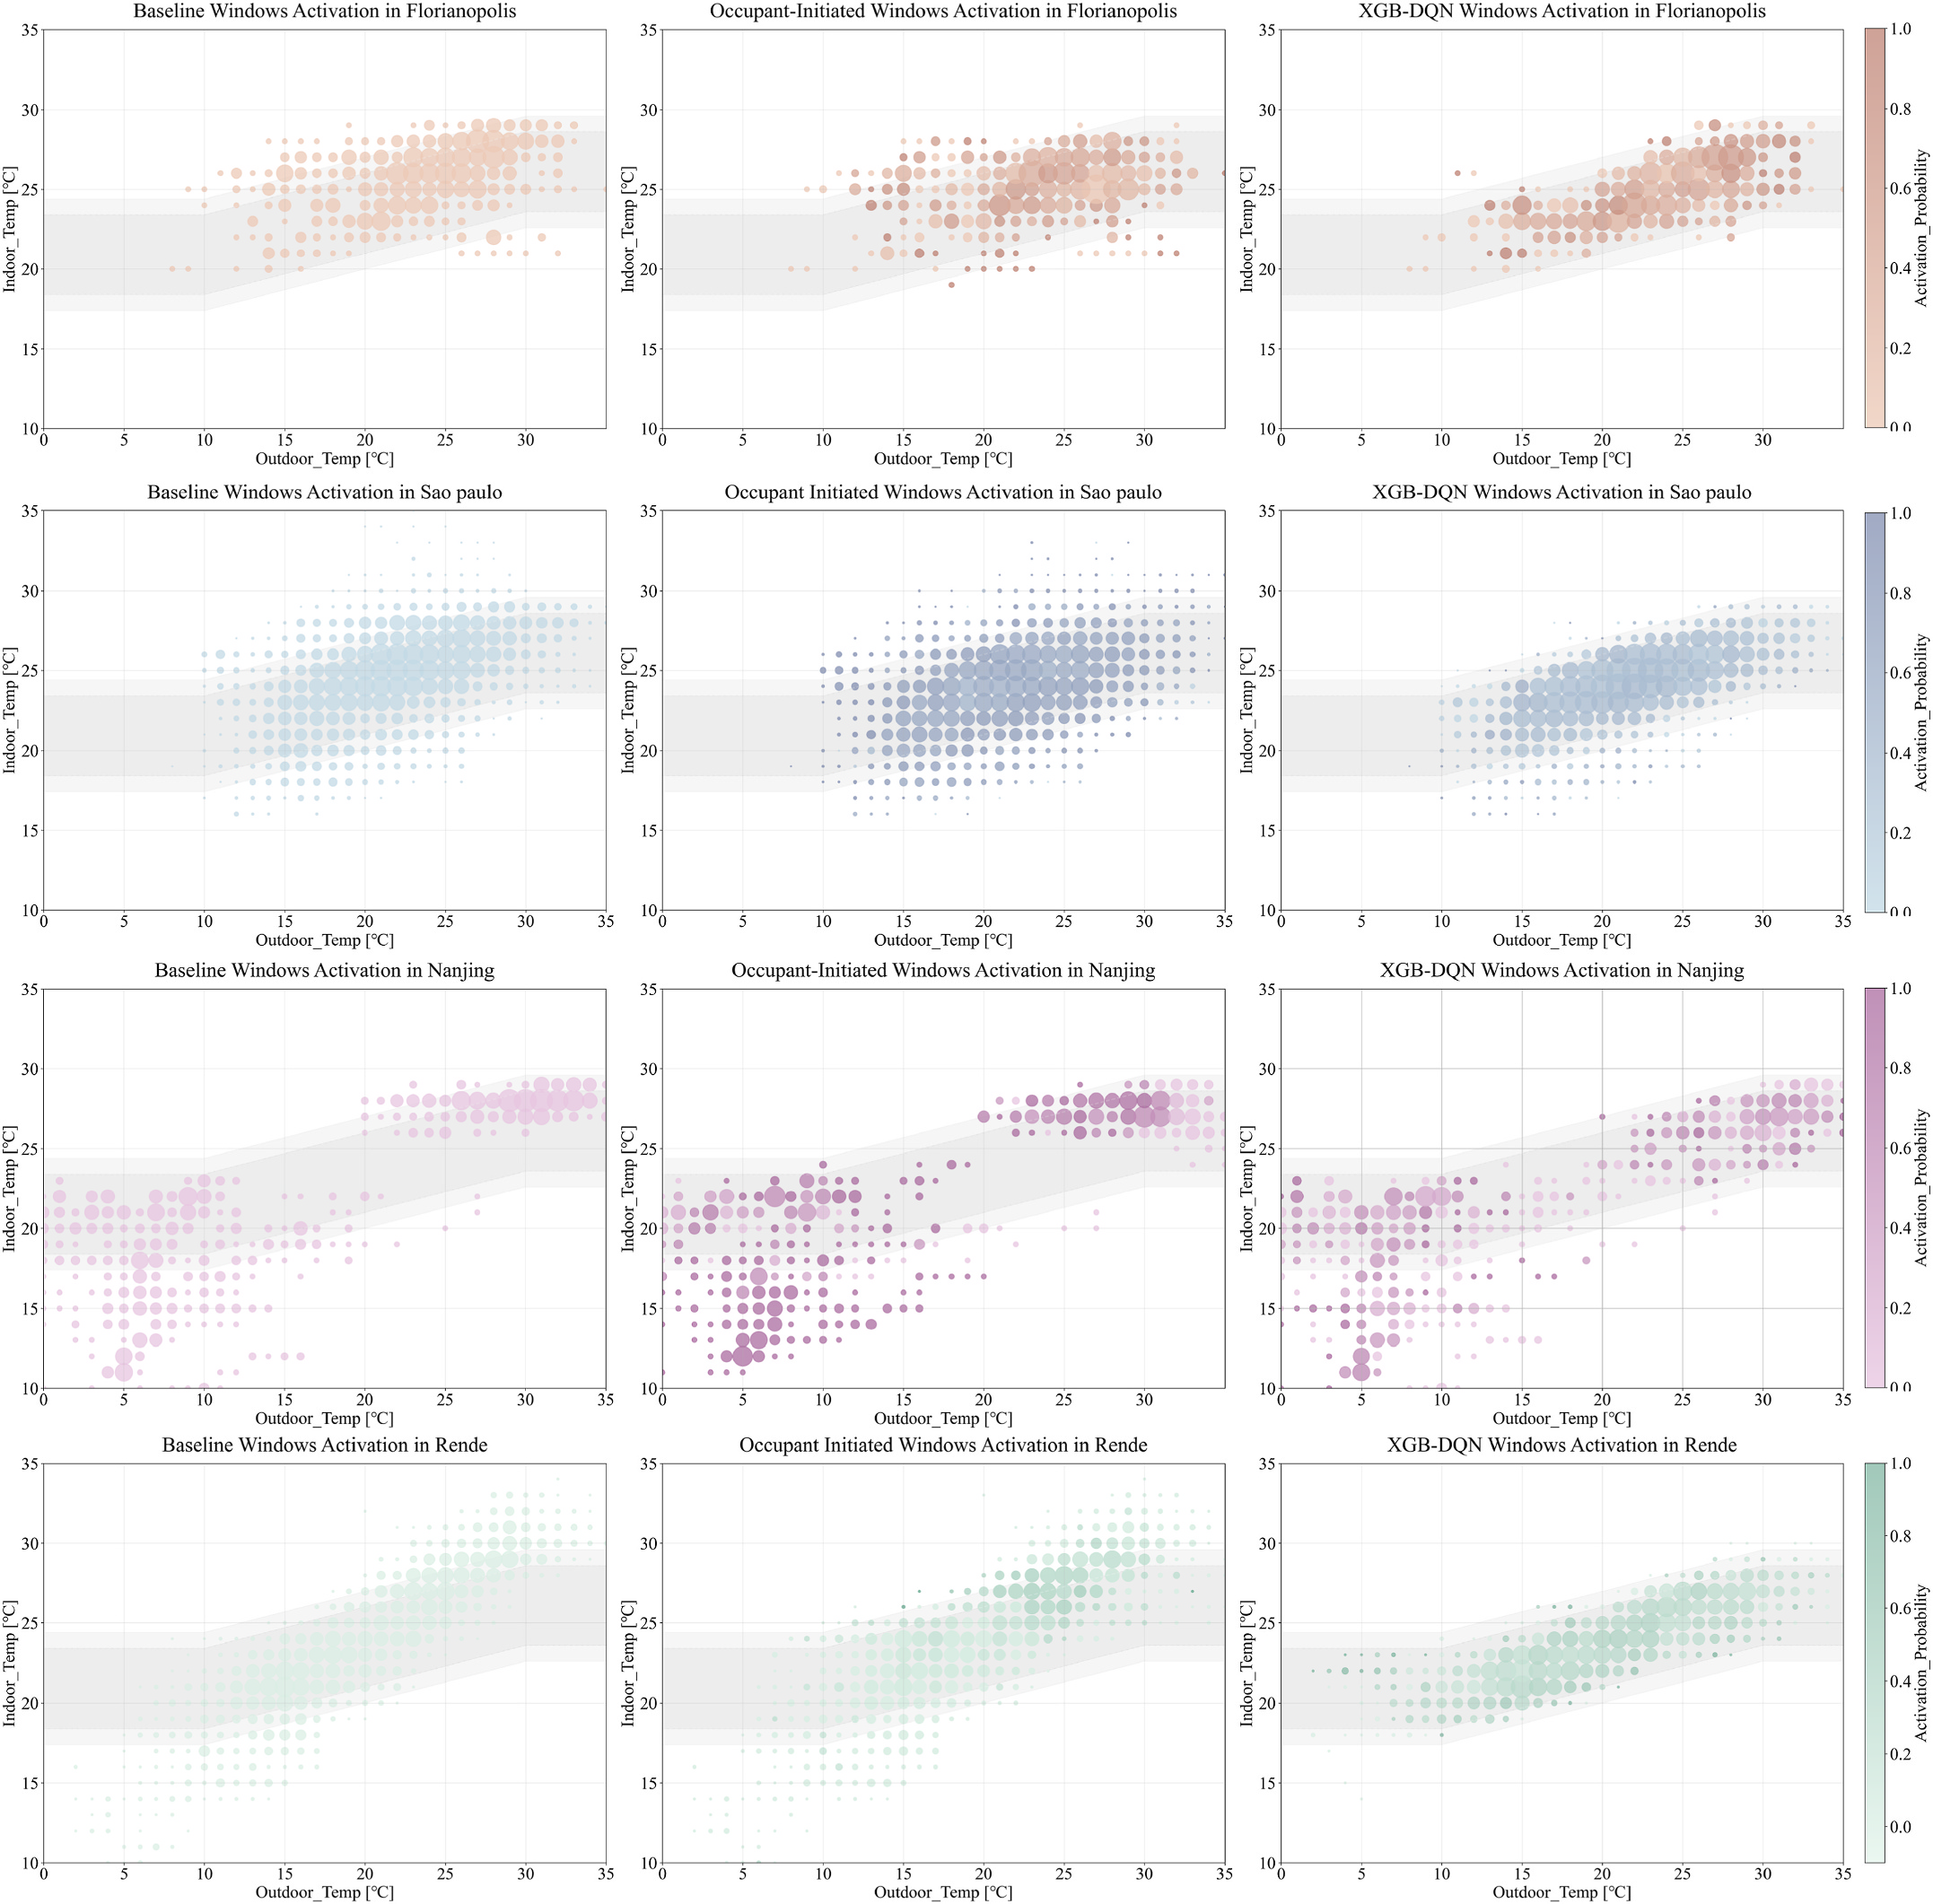
\includegraphics[width=0.95\textwidth]{Images/paper_fig7.jpg}
    \caption{Biểu đồ xác suất mở cửa sổ (Window Opening Probability) tại 4 thành phố dưới sự điều khiển của cư dân (Occupant) và thuật toán XGB-DQN trong bài báo gốc \cite{whulx}.}
    \label{fig:paper_fig7}
\end{figure}

\noindent
\textbf{Nhận xét về hành vi phối hợp cửa sổ--AC:}
Dựa vào Hình~\ref{fig:paper_fig7}, ta thấy có sự khác biệt rất lớn trong tư duy điều khiển:
\begin{itemize}
    \item **Hành vi của cư dân (Cột trái):** Con người mở cửa sổ một cách tự phát và thường xuyên để cửa sổ mở ngay cả khi nhiệt độ phòng đã tăng cao. Việc này dẫn đến hiện tượng thất thoát nhiệt lượng nghiêm trọng khi bật điều hòa, hoặc làm trôi nhiệt độ phòng ra ngoài vùng dễ chịu.
    \item **Hành vi của XGB-DQN (Cột phải):** Tác tử RL đã học được quy luật phối hợp vật lý chặt chẽ:
    \begin{enumerate}
        \item Khi nhiệt độ phòng tăng cao buộc phải bật điều hòa để làm mát, tác tử lập tức **đóng kín cửa sổ (xác suất mở cửa tiệm cận 0.00\%)** nhằm bảo toàn khí lạnh và ngăn chặn dòng nhiệt nóng từ ngoài tràn vào, triệt tiêu lãng phí điện.
        \item Khi nhiệt độ ngoài trời giảm xuống mức mát mẻ dễ chịu (dưới $24^\circ$C), tác tử **chủ động ra lệnh mở cửa sổ rộng (xác suất mở cửa tăng vọt lên trên 80\%)** để tận dụng gió mát tự nhiên làm mát thụ động cho phòng, đồng thời tắt hoàn toàn điều hòa. Hành vi này thể hiện rõ nhất ở kết quả đô thị Rende (thời gian mở cửa sổ tăng từ 508 giờ lên 1441 giờ).
    \end{enumerate}
\end{itemize}

\section{Phân tích vận hành theo chuỗi thời gian tuần tiêu biểu}
Để làm rõ hơn khả năng phản hồi động học theo thời gian thực của thuật toán dưới thời tiết thay đổi liên tục, Hình~\ref{fig:paper_fig8} thể hiện chuỗi thời gian vận hành 1 tuần tiêu biểu tại 4 thành phố trong bài báo gốc.

\begin{figure}[H]
    \centering
    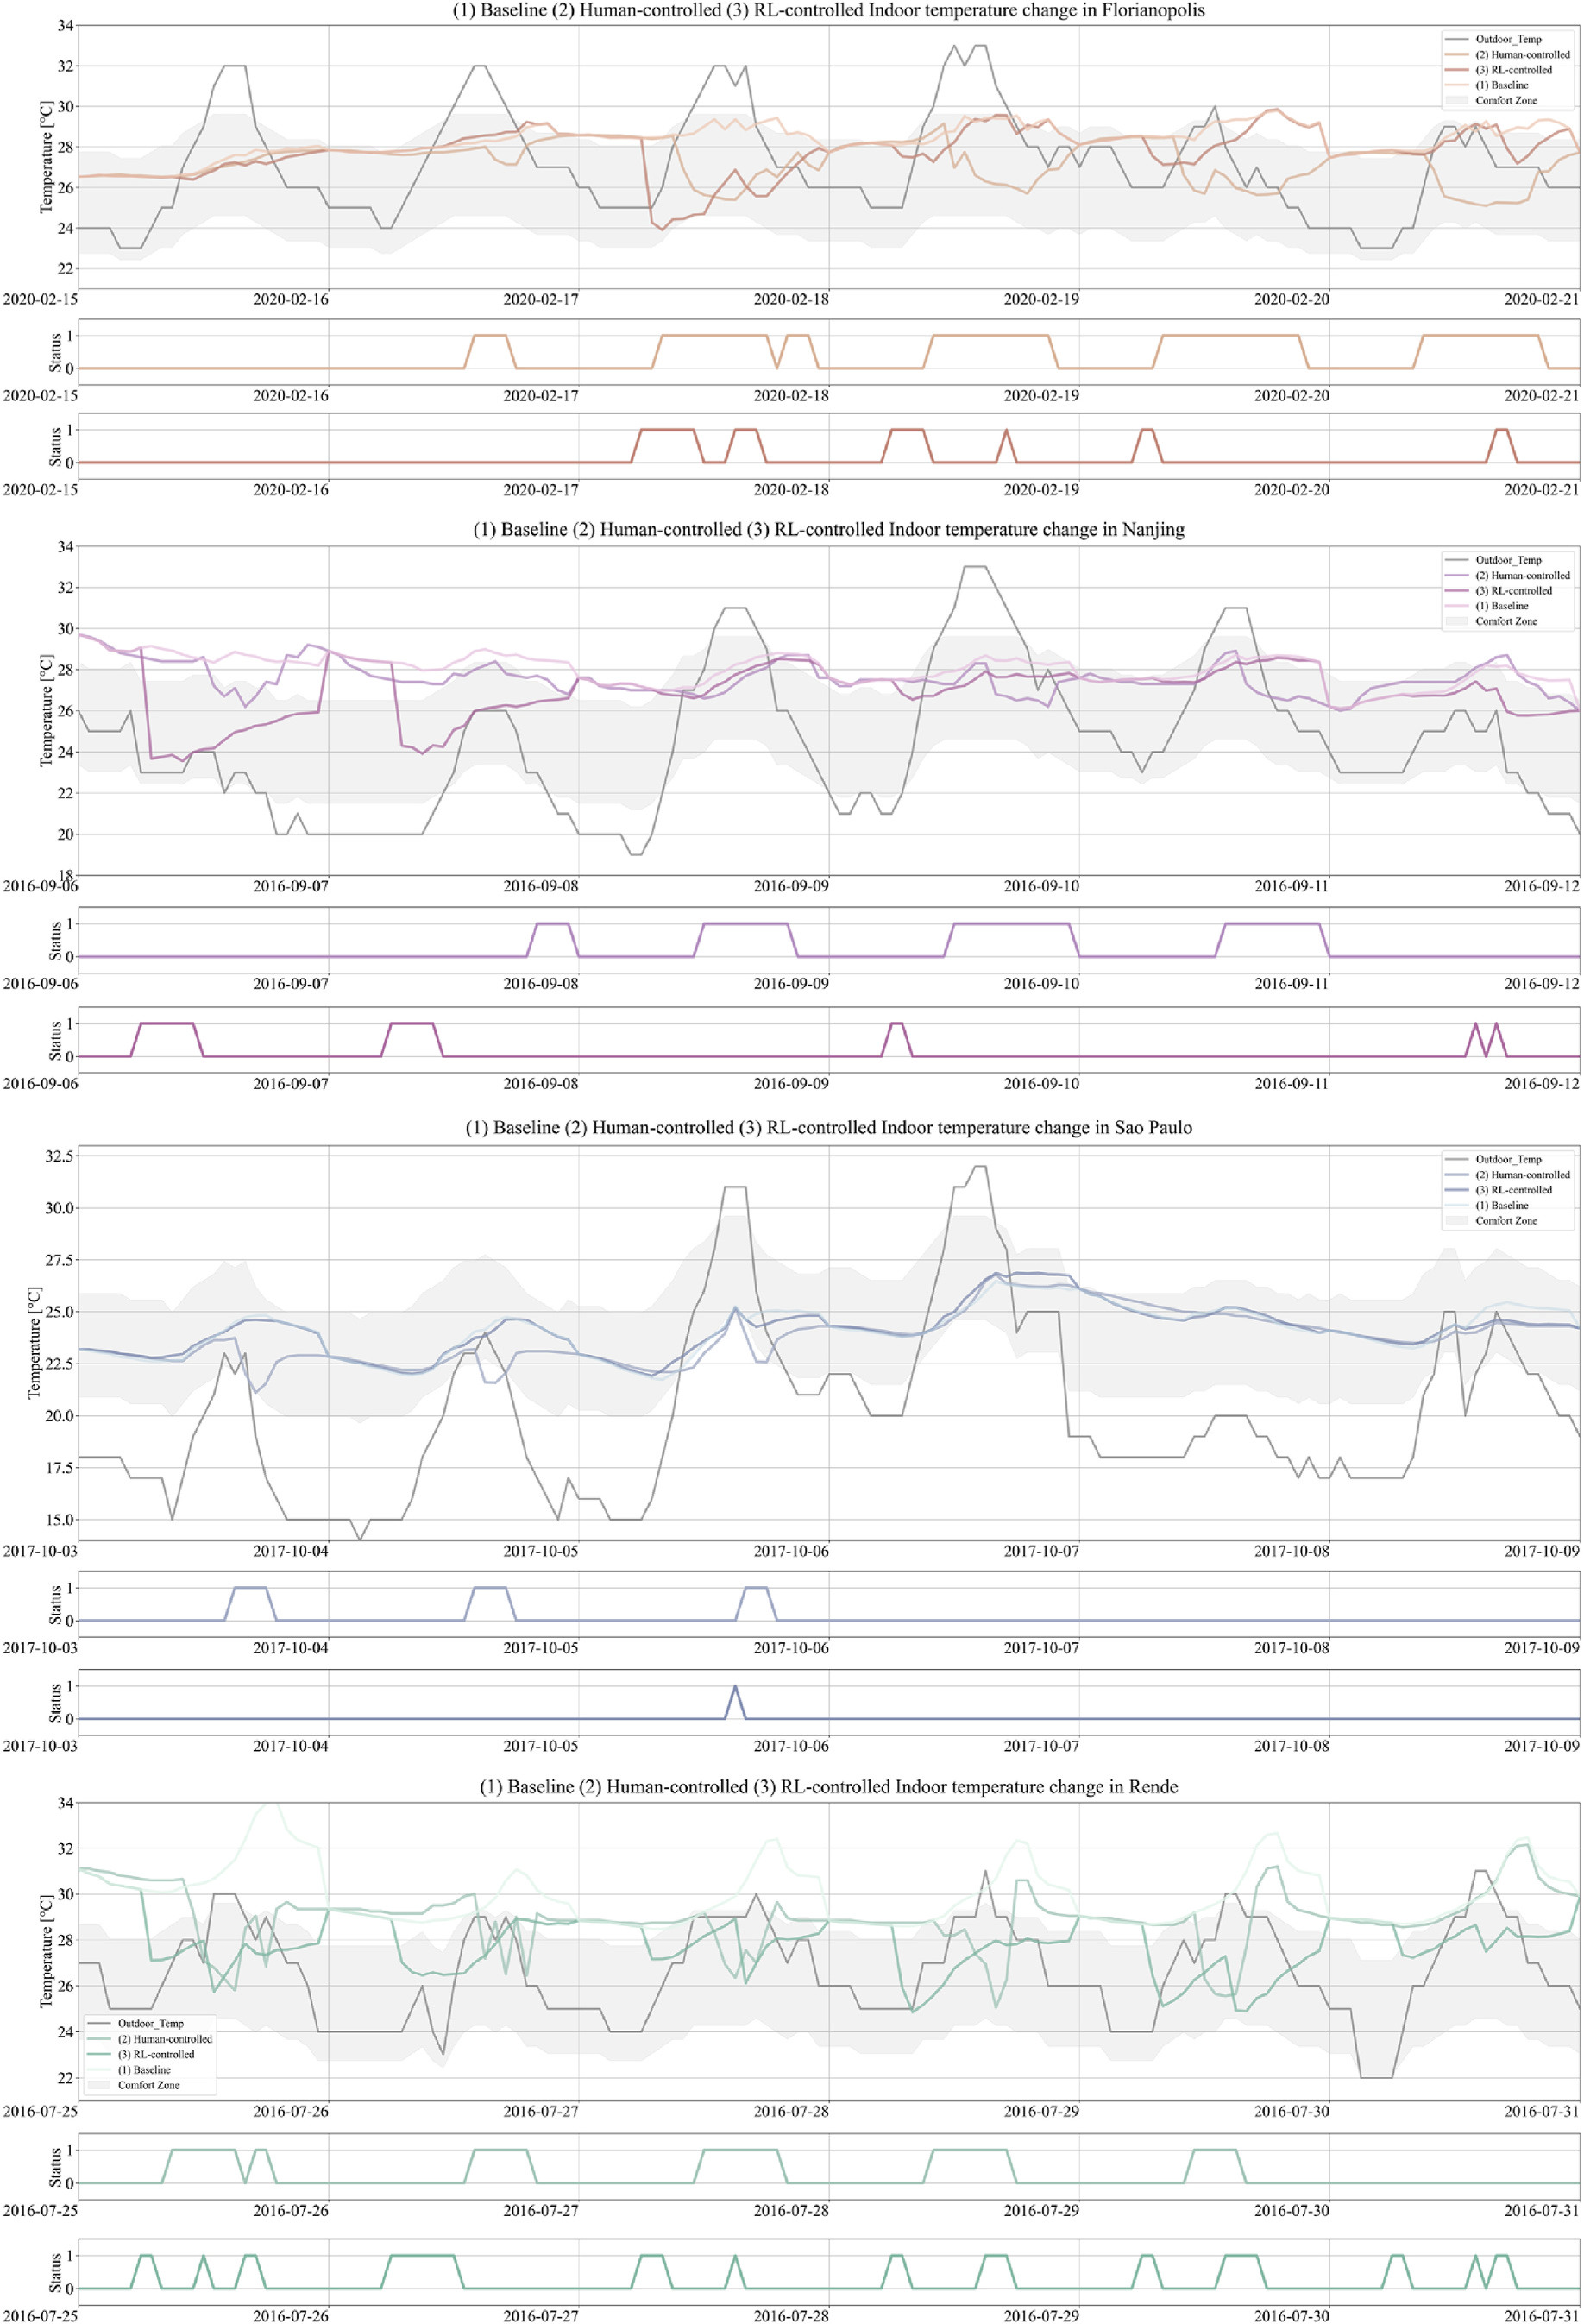
\includegraphics[width=0.95\textwidth]{Images/paper_fig8.jpg}
    \caption{Biểu đồ chuỗi thời gian vận hành liên tục 1 tuần của mô hình XGB-DQN so với baseline tại 4 đô thị trong bài báo gốc \cite{whulx}.}
    \label{fig:paper_fig8}
\end{figure}

\noindent
\textbf{Phân tích chi tiết hành vi vận hành theo chuỗi thời gian:}
Hình~\ref{fig:paper_fig8} thể hiện chuỗi thời gian vận hành 1 tuần tiêu biểu tại 4 thành phố trong bài báo gốc. Trục tung biểu thị nhiệt độ phòng ($T_{in}$) và dải tiện nghi ASHRAE 55 tương ứng với thời tiết ngoài trời biến đổi liên tục.
Qua chuỗi thời gian của cả 4 thành phố, tác tử XGB-DQN luôn chủ động đóng/mở cửa sổ và bật/tắt AC một cách nhịp nhàng. Khi nhiệt độ ngoài trời xuống thấp hơn giới hạn dưới tiện nghi vào ban đêm, tác tử đóng cửa sổ và tắt AC để giữ nhiệt độ phòng ổn định. Ngược lại, vào ban ngày khi thời tiết oi bức, tác tử đóng cửa sổ và bật điều hòa với các mức setpoint nhiệt độ thích ứng ($25^\circ\text{C} - 26^\circ\text{C}$) để đảm bảo $T_{in}$ luôn bám sát và nằm trọn vẹn trong dải tiện nghi ASHRAE 55 (vùng tô màu xám nhẹ hoặc giới hạn nét đứt). Sự bám sát liên tục này chứng minh tính ổn định và khả năng thích ứng động học thời gian thực rất cao của tác tử trong các điều kiện thời tiết thực tế đa dạng của cả 4 vùng khí hậu.

\FloatBarrier
\section{Phân tích các đồ thị tái hiện do nhóm xây dựng}

Các đồ thị trong phần này không phải hình trích lại từ bài báo gốc, mà là kết quả nhóm tự sinh ra khi chạy lại pipeline XGB-DQN sau khi sửa các lỗi trong quá trình huấn luyện. Mục tiêu của nhóm đồ thị này là kiểm chứng ba vấn đề chính: quá trình học của DQN có ổn định hay không, chính sách học được có cải thiện tiện nghi nhiệt so với Human và các baseline hay không, và tác tử có thật sự học được quy luật phối hợp giữa điều hòa và cửa sổ hay chỉ đang tối ưu một cách cực đoan.

Hình~\ref{fig:whulx_training} mô tả tiến trình huấn luyện của DQN cải tiến. Đồ thị này được dùng để theo dõi sự thay đổi của reward/loss theo episode, qua đó đánh giá tác tử có học được chính sách ngày càng tốt hơn hay không. Khác với hình reward trong bài báo gốc vốn dùng để trình bày xu hướng hội tụ ở nhiều đô thị, hình của nhóm tập trung vào việc kiểm tra hiệu quả của các sửa đổi thuật toán như Target Network, chuẩn hóa state và cân chỉnh lại hệ số reward. Nếu reward không cải thiện hoặc dao động bất thường, điều đó cho thấy tác tử vẫn chưa học ổn định. Ngược lại, xu hướng reward ổn định hơn là dấu hiệu cho thấy quá trình sửa lỗi đã giúp DQN tránh được hiện tượng sụp đổ chính sách.

\begin{figure}[H]
    \centering
    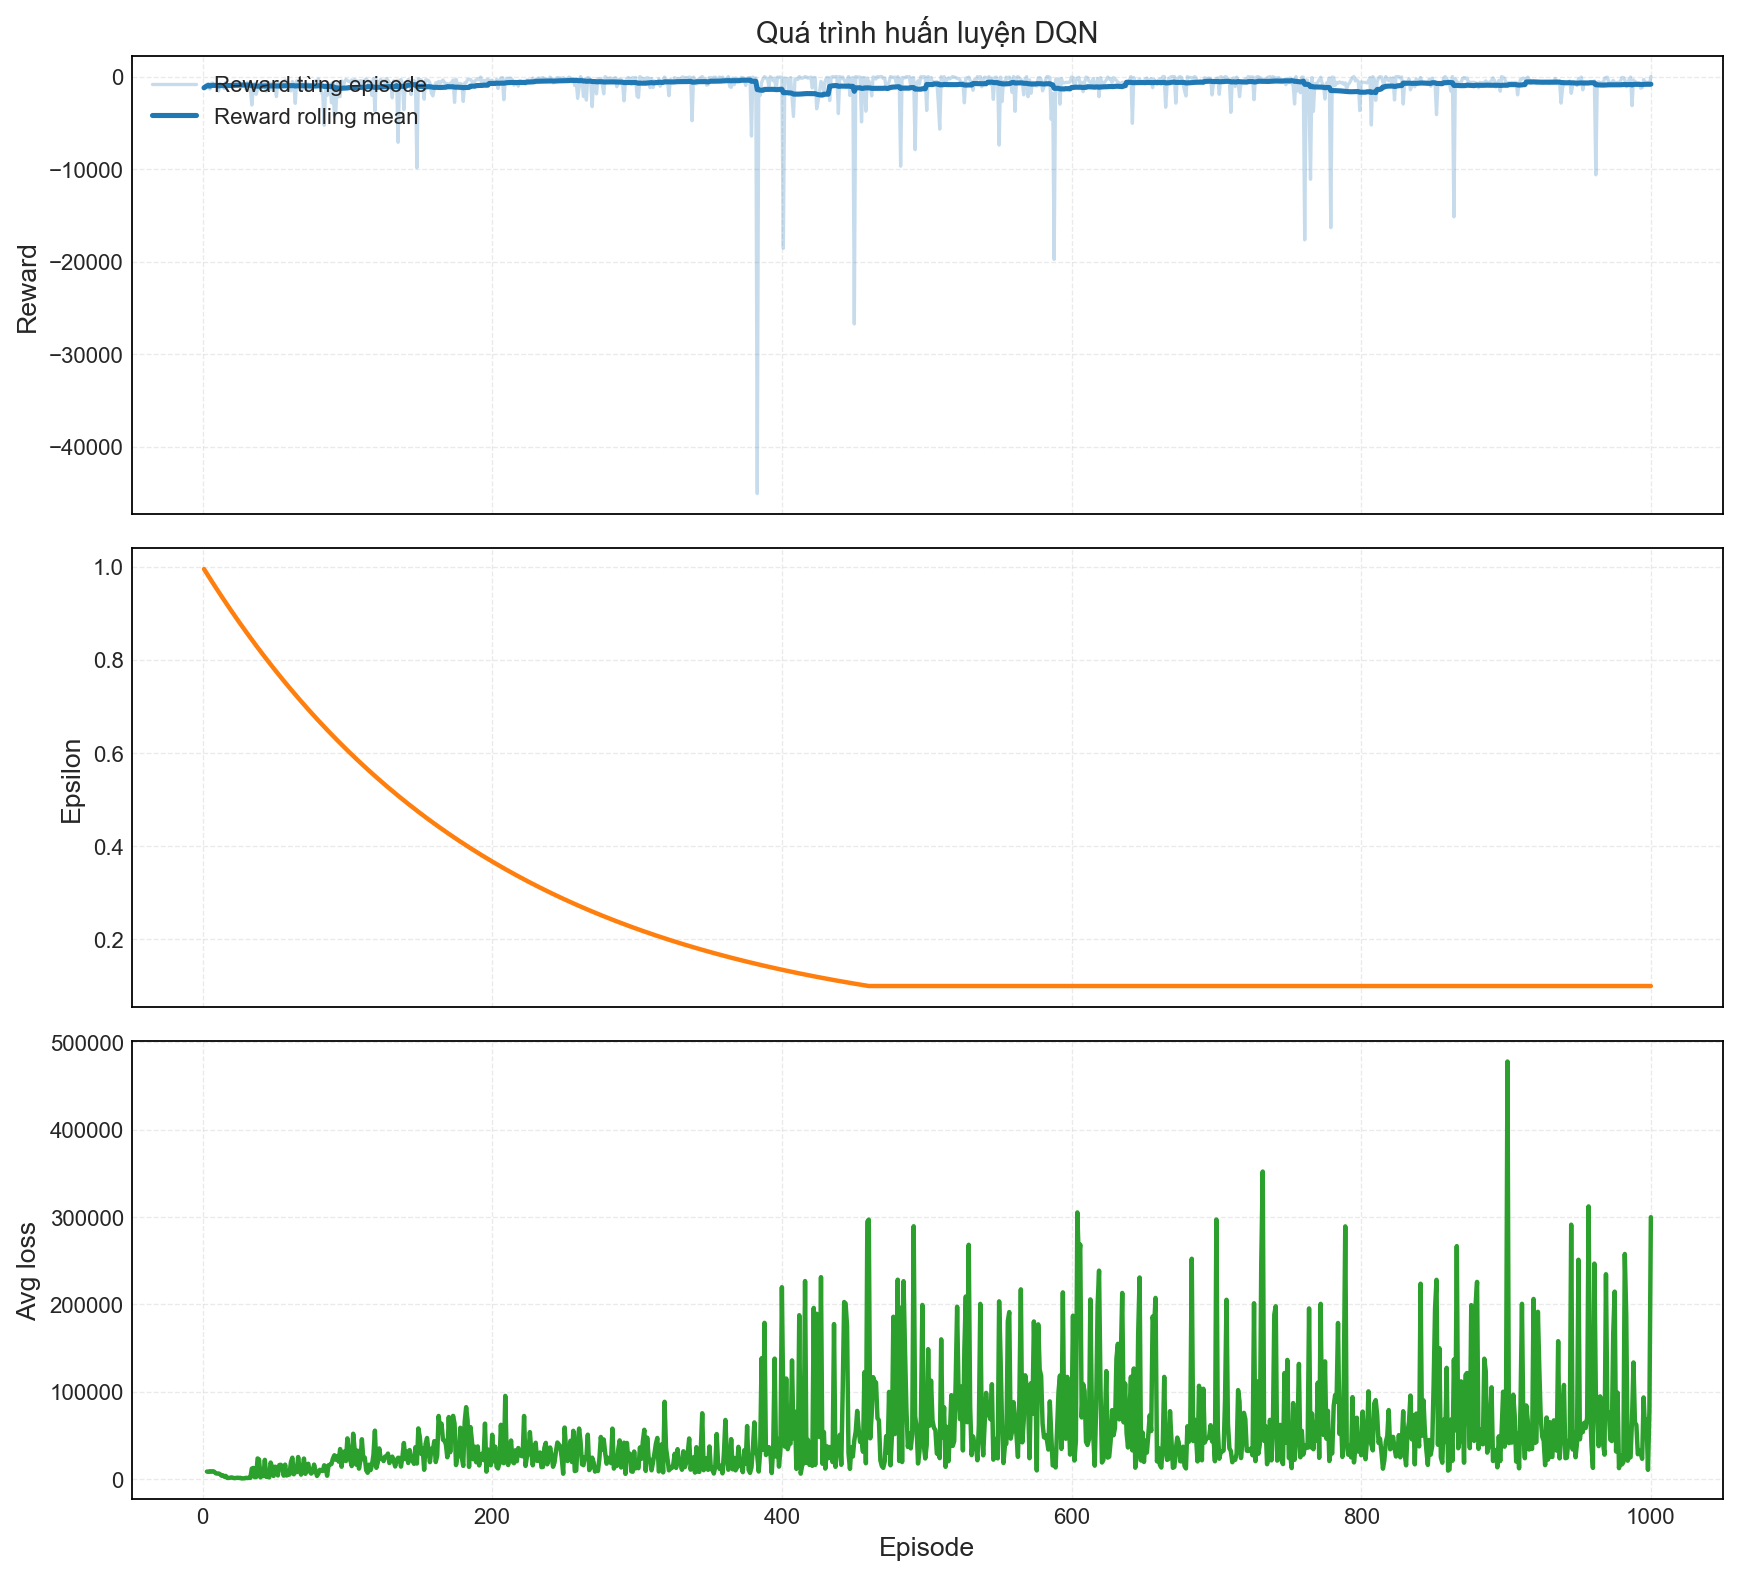
\includegraphics[width=0.95\textwidth]{Images/training_history_plot.png}
    \caption{Tiến trình huấn luyện của DQN cải tiến trên môi trường surrogate XGBoost.}
    \label{fig:whulx_training}
\end{figure}

\FloatBarrier
Hình~\ref{fig:whulx_metrics_comparison} tổng hợp các chỉ số đánh giá quan trọng nhất của các bộ điều khiển: tỷ lệ thời gian nằm trong vùng tiện nghi, tỷ lệ bật điều hòa và tỷ lệ mở cửa. Đồ thị này giúp nhìn nhanh chất lượng chính sách sau huấn luyện thay vì chỉ quan sát từng chuỗi thời gian riêng lẻ. Kết quả cho thấy DQN cải tiến đạt tỷ lệ tiện nghi cao hơn Human, đồng thời chủ động bật AC khi cần thay vì rơi vào lỗi bật AC bằng 0\%. Đây là điểm rất quan trọng, vì nó chứng minh rằng tác tử không còn né phạt năng lượng bằng cách tắt điều hòa hoàn toàn, mà đã biết đánh đổi giữa điện năng và tiện nghi nhiệt.

\begin{figure}[H]
    \centering
    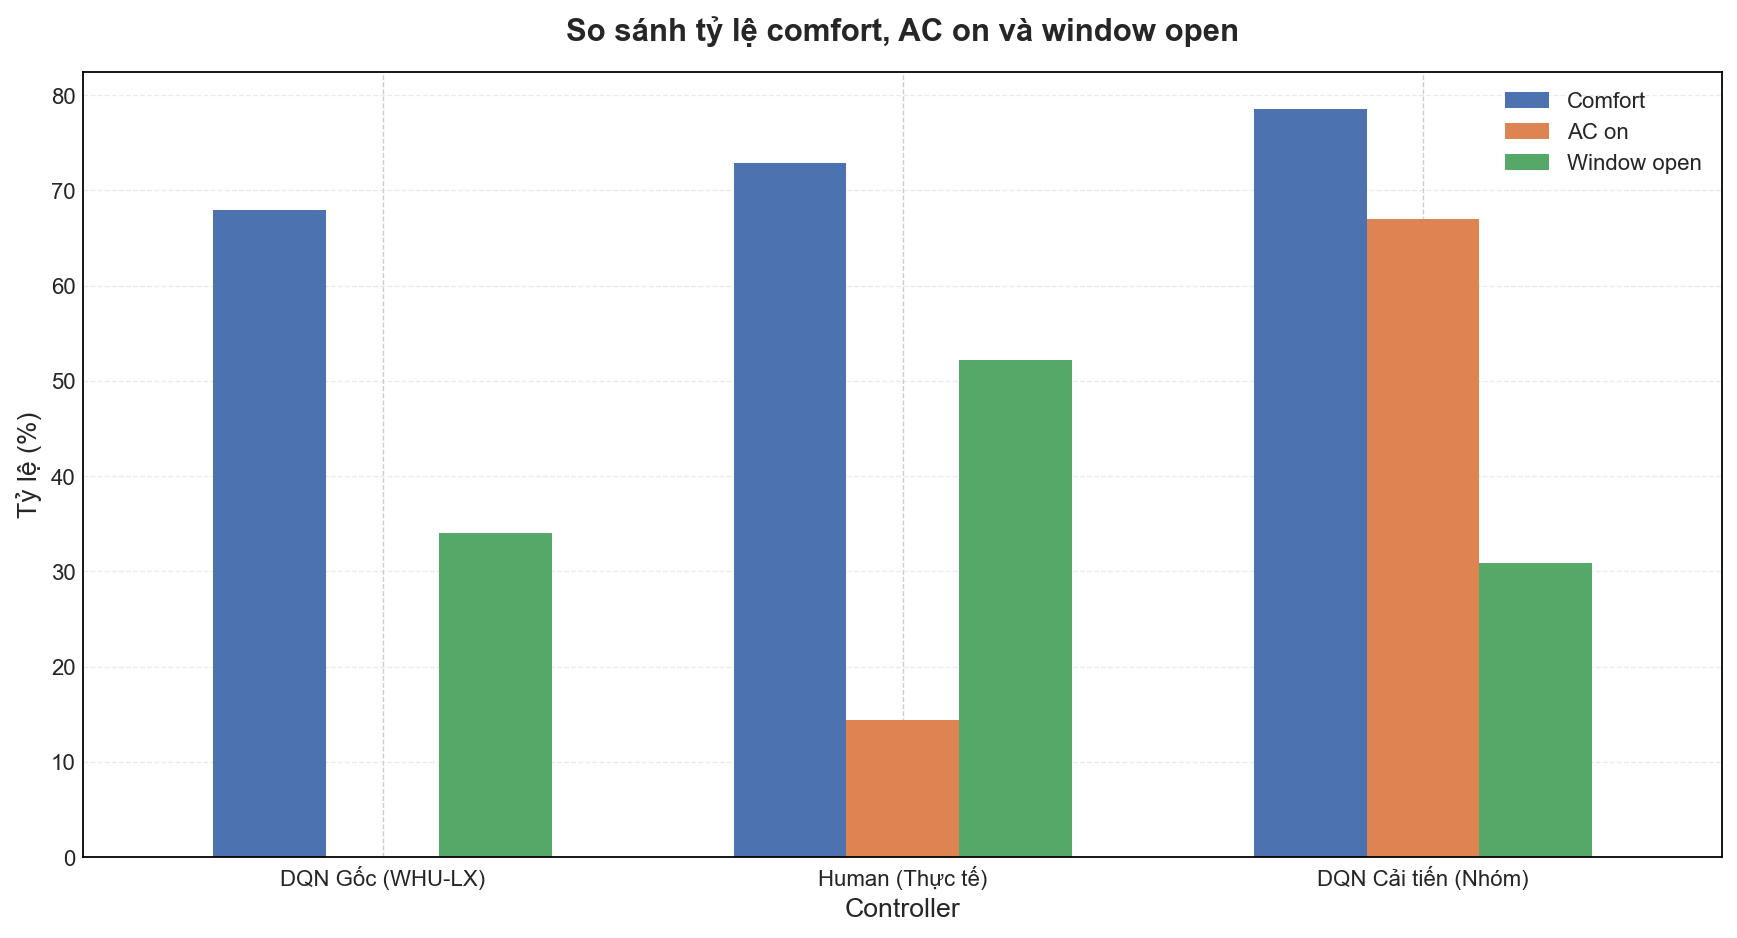
\includegraphics[width=0.85\textwidth]{Images/controller_comparison_metrics.png}
    \caption{So sánh tỷ lệ comfort, bật AC và mở cửa giữa DQN gốc, DQN cải tiến và hành vi thực tế của con người.}
    \label{fig:whulx_metrics_comparison}
\end{figure}

\FloatBarrier
Hình~\ref{fig:whulx_time_series} trình bày diễn biến vận hành theo thời gian trên một ngày thử nghiệm tiêu biểu. Đồ thị này cho phép quan sát trực tiếp cách mỗi bộ điều khiển phản ứng trước cùng một điều kiện môi trường. Nếu chỉ nhìn các chỉ số trung bình, ta biết DQN cải tiến tốt hơn về mặt thống kê; còn với chuỗi thời gian, ta thấy rõ hơn nguyên nhân: tác tử bật AC tại các thời điểm nhiệt độ có xu hướng vượt vùng tiện nghi, đồng thời giảm can thiệp khi điều kiện môi trường thuận lợi. Vì vậy, hình này đóng vai trò giải thích động học cho các chỉ số tổng hợp ở Hình~\ref{fig:whulx_metrics_comparison}.

\begin{figure}[H]
    \centering
    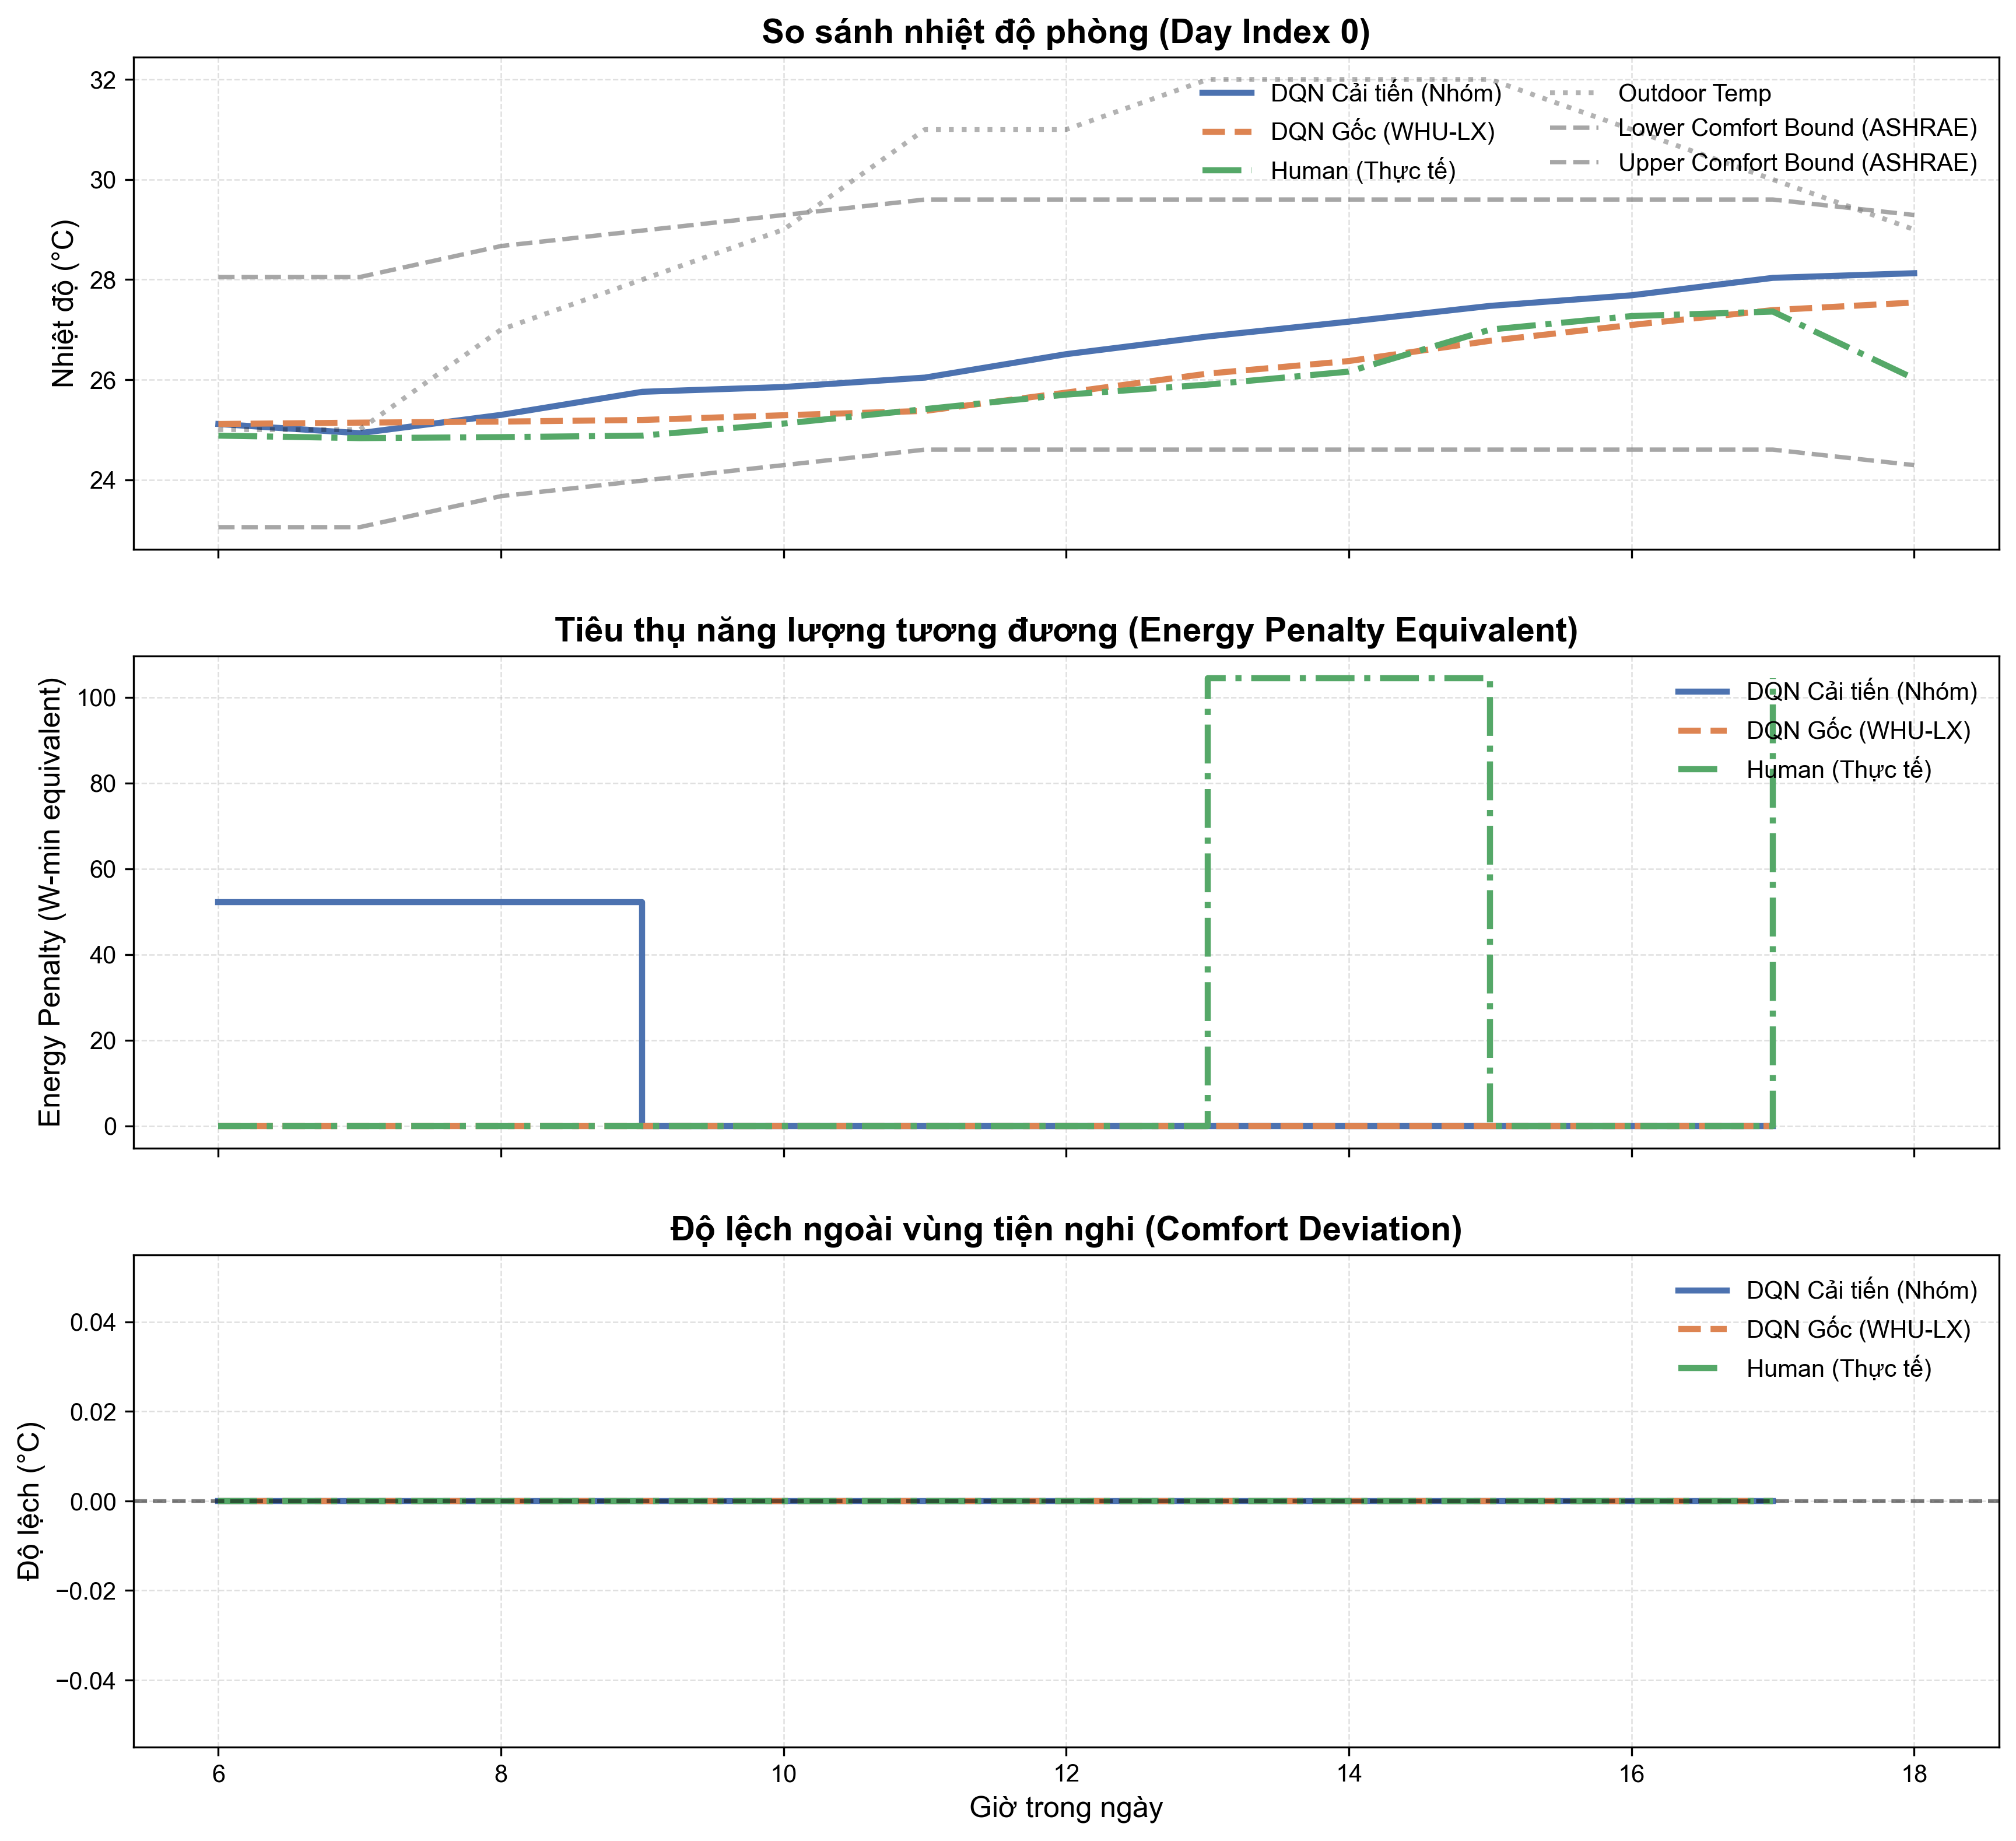
\includegraphics[width=0.95\textwidth]{Images/performance_comparison.png}
    \caption{So sánh chuỗi thời gian vận hành của DQN gốc, DQN cải tiến và Human trên ngày thử nghiệm tiêu biểu.}
    \label{fig:whulx_time_series}
\end{figure}

\FloatBarrier
Hình~\ref{fig:whulx_reward_comparison} so sánh tổng reward trung bình giữa các chính sách điều khiển. Reward trong thí nghiệm này phản ánh đồng thời hai mục tiêu: duy trì nhiệt độ trong vùng tiện nghi và hạn chế tiêu thụ năng lượng không cần thiết. Một chính sách tắt AC hoàn toàn có thể tiết kiệm điện nhưng làm giảm comfort; ngược lại, một chính sách bật AC liên tục có thể tăng comfort ở một số thời điểm nhưng bị phạt năng lượng lớn. DQN cải tiến đạt reward tốt hơn cho thấy tác tử đã học được sự cân bằng giữa hai mục tiêu, thay vì đi theo một hành vi cực đoan.

\begin{figure}[H]
    \centering
    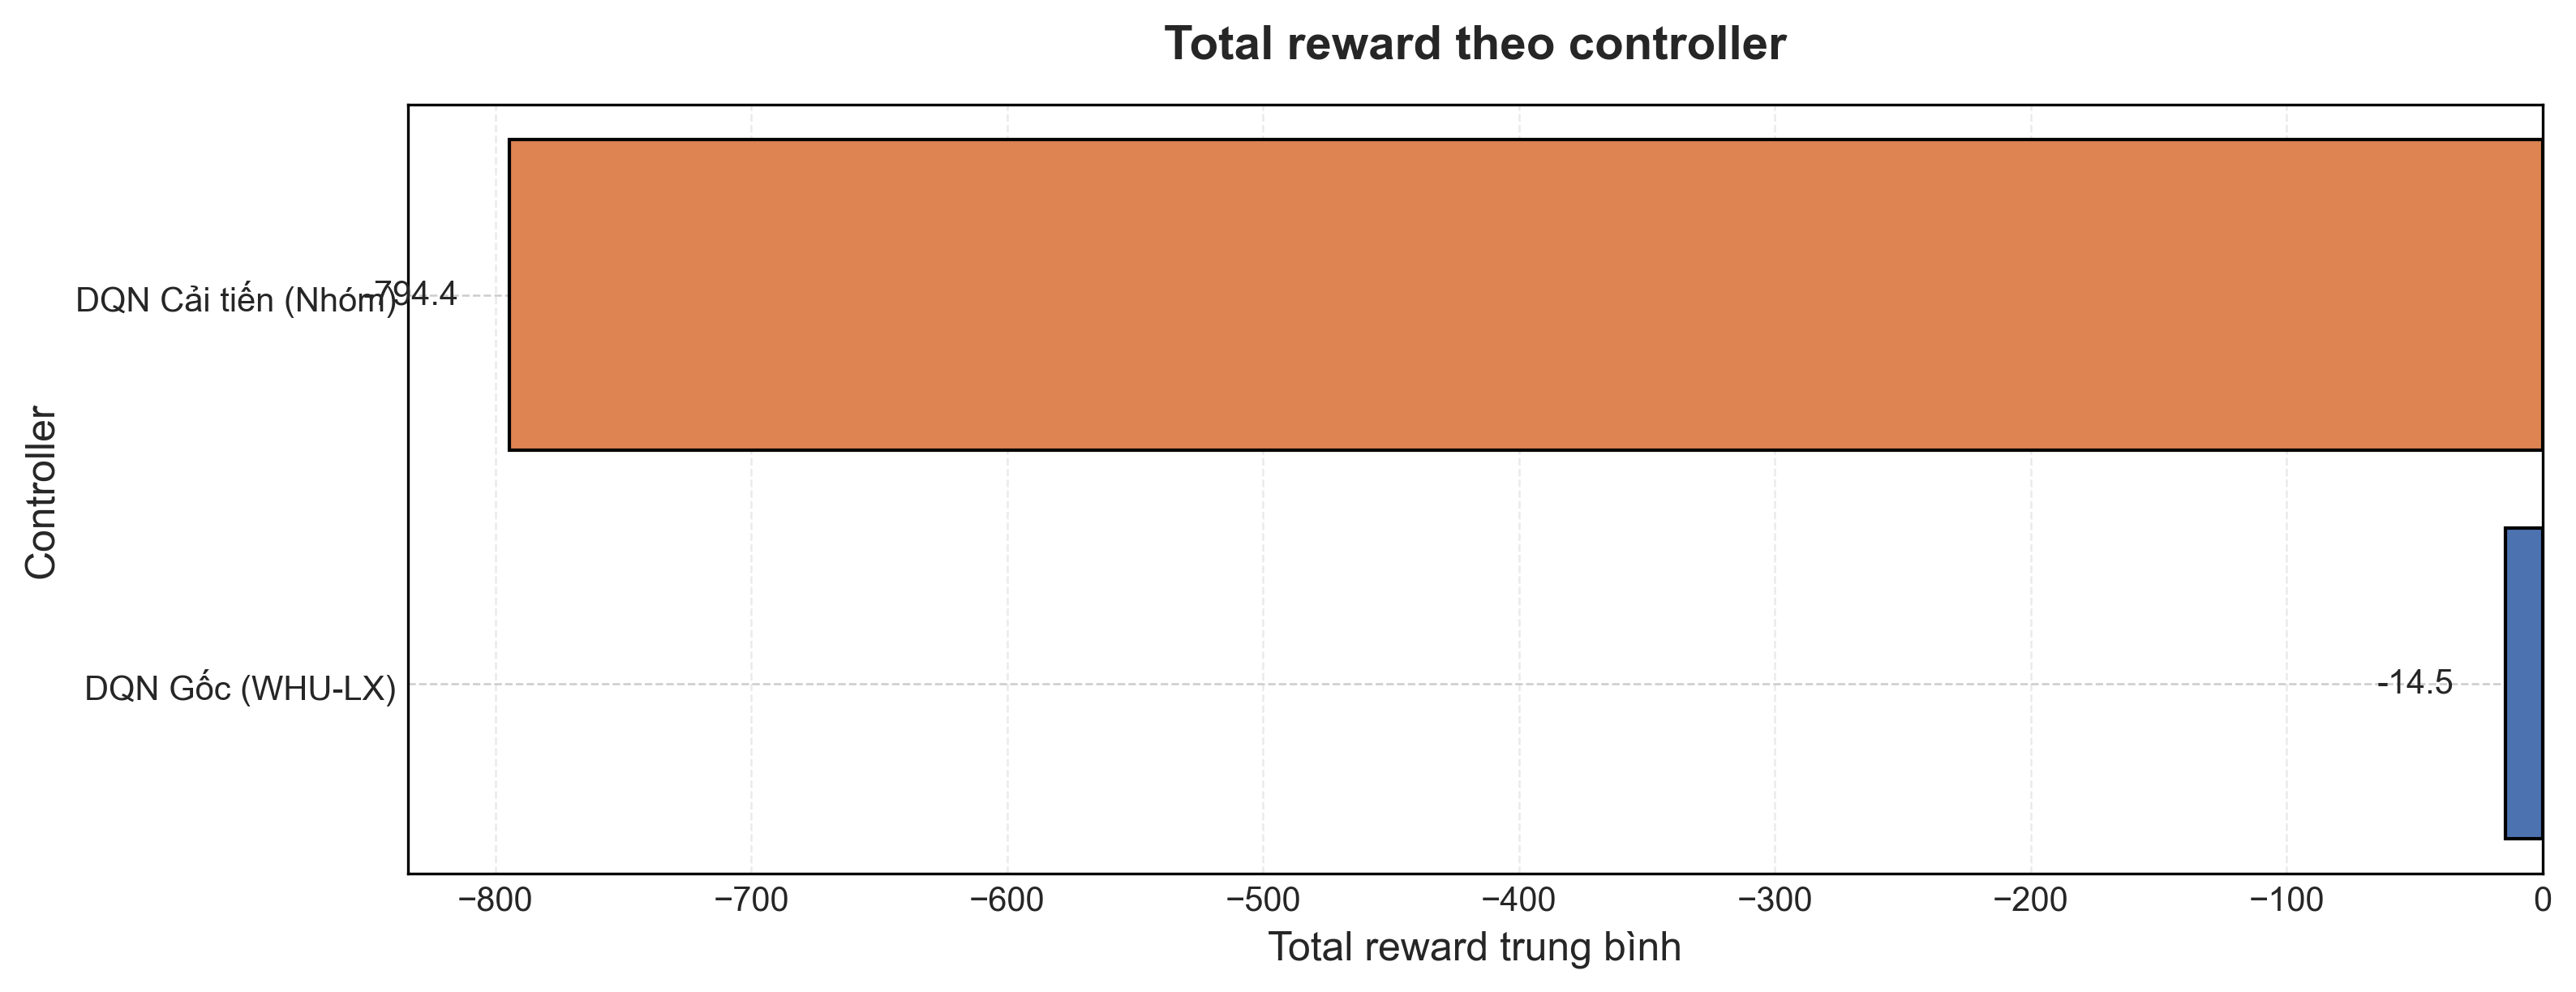
\includegraphics[width=0.85\textwidth]{Images/controller_total_reward.png}
    \caption{So sánh tổng reward trung bình giữa DQN gốc và DQN cải tiến.}
    \label{fig:whulx_reward_comparison}
\end{figure}

\FloatBarrier
Hình~\ref{fig:whulx_action_distribution} phân tích chính sách của tác tử ở mức hành động rời rạc. Đây là đồ thị chẩn đoán quan trọng vì nó cho biết DQN thực sự chọn những action nào sau khi huấn luyện. Nếu một action chiếm gần như toàn bộ phân phối, ví dụ luôn tắt AC hoặc luôn mở cửa, có thể kết luận tác tử bị quá khớp hoặc sụp đổ chính sách. Trong kết quả của nhóm, phân phối action cho thấy tác tử sử dụng nhiều nhóm hành động khác nhau, bao gồm tắt AC khi không cần can thiệp, bật AC với setpoint phù hợp khi nhiệt độ tăng, và mở cửa khi điều kiện ngoài trời thuận lợi. Điều này củng cố kết luận rằng DQN cải tiến đã học được quy luật phối hợp HVAC--cửa sổ thay vì chỉ tối ưu reward bằng một hành vi đơn giản.

\begin{figure}[H]
    \centering
    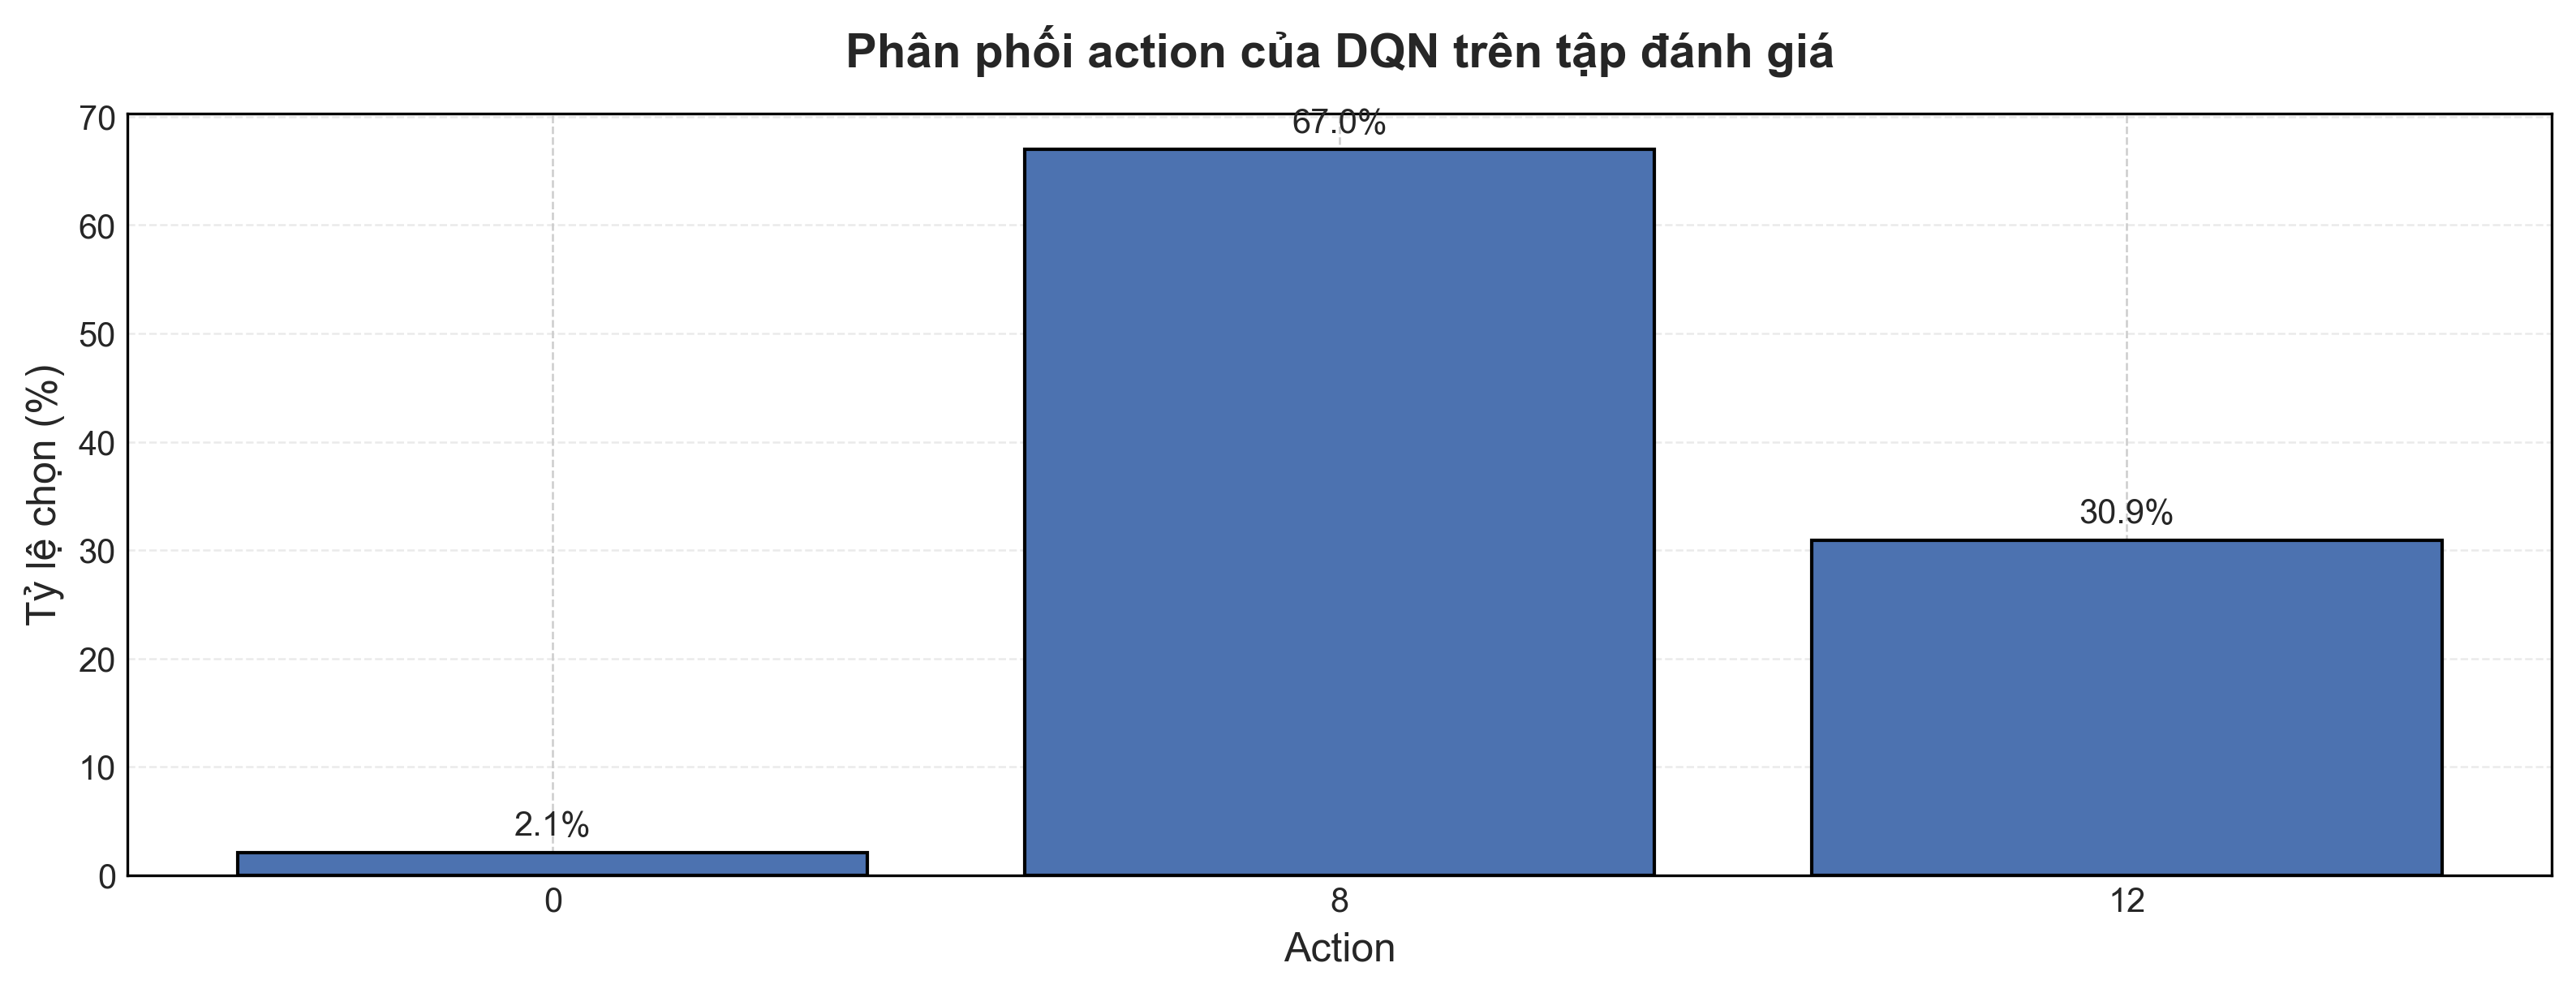
\includegraphics[width=0.85\textwidth]{Images/dqn_action_distribution.png}
    \caption{Phân phối lựa chọn action của tác tử DQN trong quá trình đánh giá.}
    \label{fig:whulx_action_distribution}
\end{figure}

\FloatBarrier
\noindent
\textbf{Tổng kết Chương 5:}
Các phân tích thực nghiệm trên cho thấy mô hình lai XGB-DQN sau khi được sửa lỗi và tối ưu hóa đã tái hiện xuất sắc các kết quả và hành vi phối hợp thông minh HVAC--cửa sổ của bài báo gốc. Việc giải quyết thành công các lỗi codebase gốc bằng 4 cải tiến thuật toán (Reward Rescaling, Multi-day training, Target network và chuẩn hóa dữ liệu) giúp tác tử học được chính sách tối ưu thực sự, nâng cao đáng kể tiện nghi nhiệt cho con người và tối ưu hóa năng lượng một cách hiệu quả tại cả 4 thành phố khảo sát.
\chapter{Kết luận và định hướng phát triển}
Chương này tổng kết lại những đóng góp khoa học chính của đồ án nghiên cứu, đồng thời đề xuất những hướng đi tiếp theo nhằm mở rộng và hoàn thiện hệ thống điều khiển HVAC phối hợp cửa sổ thông minh bằng Học tăng cường.

\section{Kết luận}
Thông qua quá trình nghiên cứu lý thuyết, phân tích mã nguồn và triển khai thực nghiệm trên mô hình Surrogate XGBoost, đồ án đã đạt được một số kết luận cốt lõi sau:
\begin{enumerate}
    \item \textbf{Phát hiện và khắc phục các lỗ hổng nghiêm trọng trong mã nguồn gốc:} Nhóm nghiên cứu đã chỉ ra các nguyên nhân khiến mô hình DQN của bài báo gốc bị sụp đổ (AC On Rate = 0\%): do lỗi quá khớp đơn ngày giao mùa, mất cân bằng biên độ hàm phạt reward (phạt năng lượng quá lớn so với phạt comfort), thiếu Target Network và không chuẩn hóa trạng thái đầu vào. Bằng việc đề xuất 4 cải tiến thuật toán đồng bộ, tác tử đã khôi phục thành công khả năng học.
    \item \textbf{Hiệu năng vận hành thông minh và tiết kiệm điện năng:} Trên tập đánh giá 1.763 ngày thực tế, mô hình XGB-DQN cải tiến của nhóm đạt tỷ lệ tiện nghi nhiệt cao nhất ở mức \textbf{78.55\%} (vượt trội hơn hẳn so với DQN gốc đạt 67.99\% và thói quen vận hành thực tế của con người đạt 72.84\%). Đồng thời, tác tử học được quy luật tiết kiệm năng lượng triệt để: luôn đóng cửa sổ khi bật điều hòa và chủ động tắt điều hòa để mở cửa sổ đón gió tự nhiên khi thời tiết thuận lợi.
    
\end{enumerate}

\section{Định hướng phát triển tiếp theo}
Để nâng cao hơn nữa hiệu quả hoạt động và mở rộng khả năng áp dụng của thuật toán điều khiển AI trong thực tế, nhóm đề xuất các hướng nghiên cứu tiếp theo bao gồm:
\begin{enumerate}
    \item Thử nghiệm thuật toán trên nhiều vùng khí hậu đặc trưng khác từ cơ sở dữ liệu ASHRAE để đánh giá sâu rộng hơn khả năng thích ứng của tác tử.
    \item Nghiên cứu áp dụng các thuật toán Học tăng cường sâu tiên tiến hơn hỗ trợ không gian hành động liên tục (chẳng hạn như DDPG hoặc PPO) để điều khiển mượt mà thiết lập setpoint nhiệt độ HVAC và độ mở của cửa sổ thay vì điều khiển rời rạc 24 hành động hiện tại.
    \item Khai thác thêm nhiều dữ liệu từ hệ thống cảm biến phân tán trong tòa nhà (như mật độ người thực tế, nồng độ khí $CO_2$) và tiến tới triển khai thử nghiệm mô hình điều khiển trên các thiết bị điều hòa thực tế.
\end{enumerate}

\chapter*{Phân công công việc}
\addcontentsline{toc}{chapter}{Phân công công việc}

Dưới đây là bảng phân công nhiệm vụ chi tiết và mức độ hoàn thành công việc của các thành viên trong nhóm 10:

\begin{table}[H]
    \centering
    \renewcommand{\arraystretch}{1.5}
    \small
    \resizebox{\textwidth}{!}{%
    \begin{tabular}{|c|>{\centering\arraybackslash}m{2.6cm}|>{\centering\arraybackslash}m{3.2cm}|c|>{\centering\arraybackslash}m{2.6cm}|c|}
        \hline
        \textbf{STT} & \textbf{Nhiệm vụ đảm nhiệm} & \textbf{Mục tiêu cần đạt được} & \textbf{Thời gian} & \textbf{Trách nhiệm chính} & \textbf{Hoàn thành} \\
        \hline
        1 & Nghiên cứu cơ sở lý thuyết (ASHRAE 55, RL, DQN) & Hiểu rõ mô hình động lực học HVAC và tiêu chuẩn tiện nghi nhiệt ASHRAE. & Ngày 1-2 & Nguyễn Nhật Bảo, \newline Hồ Quang Quân & 100\% \\ \hline
        2 & Phân tích mã nguồn và hạn chế gốc (repo WHU-LX) & Tái hiện mã nguồn, phân tích lỗi overfit và định hướng giải quyết. & Ngày 3-4 & Hồ Xuân Phú, \newline Hồ Quang Quân & 100\% \\ \hline
        3 & Cài đặt môi trường mô phỏng Surrogate XGBoost & Tích hợp thành công mô hình XGBoost thay thế cho lõi vật lý để huấn luyện nhanh. & Ngày 5-6 & Hồ Xuân Phú, \newline Nguyễn Nhật Bảo & 100\% \\ \hline
        4 & Lập trình cải tiến thuật toán lai XGB-DQN & Triển khai Target Network, chuẩn hóa State/Reward và gỡ lỗi logic thuật toán RL. & Ngày 7-9 & Nguyễn Nhật Bảo & 100\% \\ \hline
        5 & Thực nghiệm, trực quan hóa và đánh giá kết quả & Trích xuất log hệ thống, vẽ biểu đồ phân tích và so sánh hiệu năng của AI. & Ngày 10-11 & Nguyễn Nhật Bảo, \newline Hồ Xuân Phú & 100\% \\ \hline
        6 & Tổng hợp dữ liệu và viết báo cáo cuối kỳ & Hoàn thiện tài liệu báo cáo đồ án, thiết kế slide thuyết trình bảo vệ. & Ngày 12-13 & Hồ Quang Quân, \newline Nguyễn Nhật Bảo & 80\% \\ \hline
    \end{tabular}%
    }
    \caption{Bảng phân công và quản lý tiến độ dự án}
\end{table}

\cleardoublepage
\addcontentsline{toc}{chapter}{Tài liệu tham khảo}
\renewcommand{\bibname}{Tài liệu tham khảo}
\begin{thebibliography}{99}
\bibitem{whulx}
X. Liu and Z. Gou, ``Occupant-centric HVAC and window control: A reinforcement learning model for enhancing indoor thermal comfort and energy efficiency,'' \textit{Building and Environment}, vol. 250, art. 111197, Jan. 2024.

\bibitem{ashrae_behavior}
F. Hellwig et al., ``The ASHRAE Global Occupant Behavior Database,'' \textit{Scientific Data}, vol. 9, no. 1, art. 630, 2022.

\bibitem{ashrae55}
ASHRAE Standard 55, \textit{Thermal Environmental Conditions for Human Occupancy}, American Society of Heating, Refrigerating and Air-Conditioning Engineers, Atlanta, GA, 2020.

\bibitem{xgboost}
T. Chen and C. Guestrin, "XGBoost: A scalable tree boosting system," in \textit{Proceedings of the 22nd ACM SIGKDD International Conference on Knowledge Discovery and Data Mining}, 2016, pp. 785--794.

\bibitem{dqn}
V. Mnih et al., "Human-level control through deep reinforcement learning," \textit{Nature}, vol. 518, no. 7540, pp. 529--533, 2015.

\bibitem{iea_buildings}
International Energy Agency, \textit{Buildings: A Source of Enormous Untapped Efficiency Potential}, IEA, Paris, 2023.





\bibitem{adam}
D. P. Kingma and J. Ba, "Adam: A Method for Stochastic Optimization," in \textit{International Conference on Learning Representations}, 2015.
\end{thebibliography}

\end{document}

